\documentclass[12pt]{report}
\usepackage[hidelinks]{hyperref}
\usepackage[spanish]{babel}
\usepackage[utf8]{inputenc}
\usepackage{geometry}
\usepackage{graphicx}

\graphicspath{{img/}}

\newgeometry{
	right=3cm,
	left=3cm,
	top=2.5cm,
	bottom=2.5cm
}

\hypersetup{
	colorlinks,
	citecolor=black,
	filecolor=black,
	linkcolor=black,
	urlcolor=black
}

% Índice
\addto\captionsspanish{
	\renewcommand{\contentsname}%
	{Índice}%
}

\begin{titlepage}

\title{
	\begin{figure}
		\centering
			
\includegraphics[width=2cm, height=3cm]{img/logo.png}\\
			{Universidad del Bío-Bío\\
			Facultad de Ciencias Empresariales\\
			Depto. de Sistemas de Información}
	\end{figure}
	{Desarrollo de una aplicación web para la comunidad de Re-Volt America}\\
	{\large Proyecto de título para optar al título de Ingeniero de Ejecución en Computación e Informática}
}
\author{José Benavente}
\date{Viernes 6 de octubre, 2023}

\end{titlepage}

\begin{document}

\maketitle

\tableofcontents

\chapter*{Abstracto}
\addcontentsline{toc}{section}{Abstracto}
A

\chapter*{Dedicatoria}
\addcontentsline{toc}{section}{Dedicatoria}
El presente proyecto está dedicado a toda la comunidad de Re-Volt, en especial a quienes forman parte del grupo de jugadores de Re-Volt America.

Sin lugar a dudas, durante los últimos años, este juego pasó de ser un simple pasatiempo a convertirse en algo muy importante para mí a nivel personal. Muchas de las personas que he conocido a través de Re-Volt se han convertido, ya a estas alturas, en buenos amigos a quienes valoro muchísimo. Todos han sabido siempre apreciar mi trabajo, y por eso les estoy infinitamente agradecido. Sin ustedes, nada de lo que amo hacer tendría trascendencia alguna. De todo corazón, muchas gracias. Es por todo lo anterior que no podría dedicar este trabajo a nadie si no a ustedes.


\chapter*{Agradecimientos}
\addcontentsline{toc}{section}{Agradecimientos}
En primer lugar, extiendo un agradecimiento a mi profesora guía Alejandra Segura, quien ha puesto todo de su parte para ayudarme con la realización de este proyecto de título.

Quisiera también agradecer al profesor Gustavo Escobar, quien ayudó enormemente en la confección del apartado económico de este proyecto.

También extiendo un agradecimiento a la Universidad del Bío-Bío, especialmente a la facultad de ciencias empresariales y su decana Elizabeth Grandón, quien ha tenido gran incidencia en mi formación como profesional.

Se extiende también un agradecimiento formal a las siguientes personas quienes, de una forma u otra, han contribuido al presente proyecto. ¡Muchísimas gracias por todo su apoyo!.

\begin{itemize}
	\item Marco Roth, por ayudar con la migración del proyecto a ''esbuild'', y por resolver problemas con HAML.
	\item Nicolás Duque, por probar la instalación del proyecto en plataformas de Linux, testear el proyecto en su fase beta, y por ayudar con la implementación de traducciones.
	\item Luigi Riccio, por prestar su ayuda y conocimientos matemáticos para la confección y corrección de notaciones de fórmulas y funciones. 
	\item Esteban Martinez, por ayudar con la mejora de la resolución de los assets del proyecto.
	\item Henrique Gomes Britos, por ayudar con el diseño de la plataforma y selección de tipografía, además de la lectura y correción ortográfica.
  \item Felipe Pavez Sepúlveda, por ayudar con la lectura y corrección ortográfica.
\end{itemize}

Además, quisiera extender un agradecimiento a todos mis compañeros de carrera, en especial a los del grupo Bilderberg, junto con los miembros de la comunidad de Open Source UBB. Sin ustedes, mi paso por la universidad no hubiese sido igual.

También se les extiende un agradecimiento a todos quienes han hecho una donación voluntaria, sin importar el monto que fuese, a través de GitHub Sponsors durante el desarrollo de este proyecto:
\begin{itemize}
  \item Vicente Aguilera.
  \item Gabriel Carnielli.
  \item Dario Chaile.
  \item Benjamín Contreras.
  \item Benjamín Ferrada.
  \item Josafat Jiménez.
  \item  Mateusz Kobylański.
  \item Jorge Matamala.
  \item Benjamín Mosso.
  \item Leandro Rodríguez.
  \item Juan Pablo Rosas.
\end{itemize}


\chapter*{Resumen}
\addcontentsline{toc}{section}{Resumen}
VENDER REVOLT AMERICA:

RV AMERICA HA QUEDADO ATRAS EN CUANTO A SU SOPORTE Y GRACIAS A ESTE PROYECTO CRECERÁ Y SE VOLVERÁ MÁS MASIVO ETC...


El presente informe trata de una aplicación que busca centralizar toda la información relacionada a las sesiones multijugador del videojuego Re-Volt celebradas por la comunidad de Re-Volt America, la cual busca mejorar la experiencia de usuario para los administradores encargados de mantener los registros de resultados y tablas de puntuación de Re-Volt America actualizadas, además de servir como un cambio revolucionario para todos aquellos que buscan conseguir una experiencia competitiva dentro del videojuego. 


\chapter*{Introducción}
\addcontentsline{toc}{section}{Introducción}
Dentro de las comunidades del videojuego de carreras Re-Volt, 1999, Re-Volt America se ha quedado atrás en lo que refiere a su sistema interno de cálculo de resultados y estadísticas por jugador. Esta problemática genera el surgimiento de este proyecto, el cual pretende modernizar y mejorar la gestión interna de Re-Volt America, así como también busca enriquecer la experiencia de usuario como nunca antes se ha visto en la escena de las comunidades de Re-Volt.

El presente informe trata de una aplicación que busca centralizar toda la información relacionada a las sesiones multijugador del videojuego Re-Volt celebradas por la comunidad de Re-Volt America, logrando así mejorar la experiencia de usuario para los administradores encargados de mantener los registros de resultados y tablas de puntuación, además de servir como un cambio revolucionario para todos aquellos que buscan conseguir una experiencia competitiva dentro del videojuego. 


% Estudio del Problema
\chapter{Estudio del Problema}

\section{Definiciones, Siglas y Abreviaciones}
A continuación, se definirán algunos conceptos relevantes en el contexto del videojuego Re-Volt y de la comunidad de Re-Volt America:

\begin{itemize}
	\item Re-Volt: El videojuego Re-Volt, publicado por Acclaim Studios en 1999.
	\item RV: Abreviación para ''Re-Volt''.
	\item Re-Volt: OpenGL: Reescritura moderna de Re-Volt, basada en OpenGL.
	\item RVGL: Abreviación de ''Re-Volt: OpenGL''.
	\item Re-Volt I/O: Comunidad europea de Re-Volt.
	\item Re-Volt America: La comunidad americana de Re-Volt.
	\item RVA: Abreviación para ''Re-Volt America''.
	\item Sesión: Serie de carreras de RVGL en línea, en donde dos o más personas compiten en carreras multijugador.
	\item Session Log: Archivo separado por comas, el cual contiene un registro crudo de los resultados de las carreras jugadas en una sesión de RVGL.
\end{itemize}

\section{Historia de Re-Volt y sus Comunidades}
Re-Volt America, en su expresión más simple, es una comunidad de jugadores del videojuego Re-Volt, el cual fue lanzado originalmente en el año 1999 por Acclaim Studios en Londres. Re-Volt es un videojuego de carreras y simulador arcade de autos a control remoto, el cual explora una premisa en donde dichos autos compiten en carreras de radio control en ambientes como museos, supermercados, barcos, sitios de construcción, entre otros. Esto combinado con una mecánica de objetos que pueden ser recogidos por dichos autos para atacar a los competidores, obtener más velocidad, entre otras ventajas.

El arte original de la caratula del juego puede ser apreciado en la figura FIGNUM.


\includegraphics{img/re-volt.jpg}

El primero de septiembre del año 2004, Acclaim Studios se declara en banca rota, y cesa permanentemente todo el desarrollo y mantenimiento que en algún momento proveyó a Re-Volt y a su comunidad. Este suceso, a lo largo de los años, dio lugar a muchas comunidades segmentadas del juego en el internet de ese entonces. Con el tiempo, nuevos sitios y proyectos comenzaron a surgir, tales como el portal web de Re-Volt Race, una página de Re-Volt que se dedicaba a organizar partidas online y mantener tablas de resultados para los jugadores, o Re-Volt: OpenGL (RVGL), una re-escritura moderna del Re-Volt original que todos conocían, ahora disponible para plataformas modernas y otros sistemas operativos además de Windows, como Linux, MacOS, e incluso una versión para dispositivos Android.

Dentro de lo anteriormente enmarcado, aparece en el año 2015 la comunidad de Re-Volt I/O, cuyo logotipo se puede apreciar en la figura FIGNUM. Esta comunidad estaba formada por un grupo de jugadores de Re-Volt, principalmente europeos, quienes incursionaron por primera vez en intentar crear una plataforma estable para el videojuego y su comunidad de jugadores. Este sería un lugar en donde cualquiera que quisiera disfrutar del juego podría encontrar guías de ayuda, tutoriales, descargas y demás contenido para poder instalar y jugar Re-Volt en su computador o dispositivo móvil.


\includegraphics{img/io.png}

En sus inicios, Re-Volt I/O adoptó a RVGL como la distribución estándar de Re-Volt que ofrecería a sus jugadores, haciéndole ganar público y reconocimiento al proyecto publicando enlaces de descarga directos en su página web (re-volt.io), además de entregar soporte y mantener hilos de discusión relacionados con RVGL y sus actualizaciones en su foro oficial (forum.re-volt.io).

En adición a lo anterior, RVGL no era tan sólo una versión modernizada del Re-Volt original, sino que también traía consigo el aspecto más importante que tiene Re-Volt en la actualidad, y el cual mantiene unida y activa a su comunidad en general: el modo multijugador u online. Dicho modo no sólo permitía a los jugadores correr carreras en línea, sino que, además, extendía soporte para que miembros de la comunidad pudiesen diseñar sus propios autos y pistas de manera personalizada, agrandando así, de manera casi infinita, el repertorio de contenido descargable para Re-Volt.

Re-Volt I/O adoptó un sistema en donde su administración elige ciertos autos y pistas hechos por la comunidad cada ciertos meses. De esta forma, todos estos autos y pistas, elegidos a votación, terminan juntos en un paquete de contenido de extensión para RVGL, el cual Re-Volt I/O se encarga de distribuir para que sus usuarios lo descarguen y puedan jugar en línea. De manera habitual, tener este paquete de contenido es obligatorio para poder jugar en las sesiones multijugador organizadas por Re-Volt I/O, lo cual lo convertiría en un estándar para los jugadores que quisieran incorporarse a la comunidad en toda su extensión.

Fue así como Re-Volt I/O, entre finales del 2015 y mediados del 2017, logró consolidarse y llegar a más jugadores que nunca, formando una comunidad activa de amantes del juego quienes, espontáneamente, se reunían a jugar en línea durante la semana utilizando un paquete de contenido adicional para RVGL, el cual todos debían descargar e instalar por separado para poder jugar. Eventualmente, estas partidas en línea adquirieron un horario definido con fechas y horas acordadas con antelación, para así facilitar la asistencia de los jugadores a los eventos de carreras.

En la actualidad, Re-Volt I/O sigue siendo la comunidad de Re-Volt más grande en términos de jugadores y escala, pero en si todas las comunidades de Re-Volt están unidas y se ayudan unas con otras. Después de todo, se trata de un juego nicho, en donde todos intentan hacerlo accesible y fácil de entender para quienes deseen formar parte de su comunidad.

\section{La Comunidad de Re-Volt America}
Si bien Re-Volt I/O fue, durante muchos años, la única comunidad grande de Re-Volt a nivel mundial, no fue mucho después de su gran auge que comenzarían a formarse los demás grupos que, a día de hoy, tienen gran relevancia en la escena multijugador de Re-Volt y que, además, cuentan con un numeroso público y gran actividad. Dentro de estas nuevas comunidades se encuentra Re-Volt America, la comunidad de Re-Volt que abarca a todos los jugadores del continente americano, especialmente de latinoamérica. El logotipo oficial de Re-Volt America, o RVA para abreviar, puede apreciarse en la figura FIGNUM.


\includegraphics[width=10cm, height=10cm]{img/rva.png}

La comunidad de Re-Volt America es concebida originalmente en el año 2017, bajo el nombre de Re-Volt Tournament. No fue hasta después de un par de años que esta sería renombrada a Re-Volt America, debido a la procedencia de sus jugadores, la cual era tanto de norte america como de sudamerica.

En el presente año 2023, Re-Volt America cuenta con una gran cantidad de jugadores activos, y con un sistema de puntuación único en la escena de Re-Volt y sus comunidades en línea. Este complejo sistema de puntuación, y su funcionamiento sostenido durante los últimos 6 años, son la base del problema que busca solucionar este proyecto de título. Con el pasar del tiempo, este sistema se ha convertido en algo muy difícil de mantener para los administradores de la comunidad, tanto a nivel logístico como técnico.

\section{Contexto del Problema}

\subsection{Re-Volt y Partidas en Línea}
Como ya se mencionó anteriormente, Re-Volt es un videojuego de carreras el cual, gracias al surgimiento de RVGL y sus comunidades impulsoras, es jugado mayoritariamente en línea. Pero, ¿a qué nos referimos con ''jugar en línea''?. Para poder entender este concepto, tenemos que ir a lo que es una carrera en términos conceptuales, y las implicaciones que estas conllevan dentro de un contexto competitivo.

Para poder jugar en línea, cada jugador debe elegir un nombre de usuario, el cual puede incluso variar de partida en partida. Esto se hace una vez que ingresa al juego y avanza en el menú hasta llegar al selector de nombre de usuario en forma de neumático. El nombre que el jugador ingrese aquí será el nombre de usuario con el que se identificará a la hora de ser ingresado a los resultados de cada carrera en la que participe. El selector de nombre de usuario se puede apreciar a continuación en la figura FIGNUM.

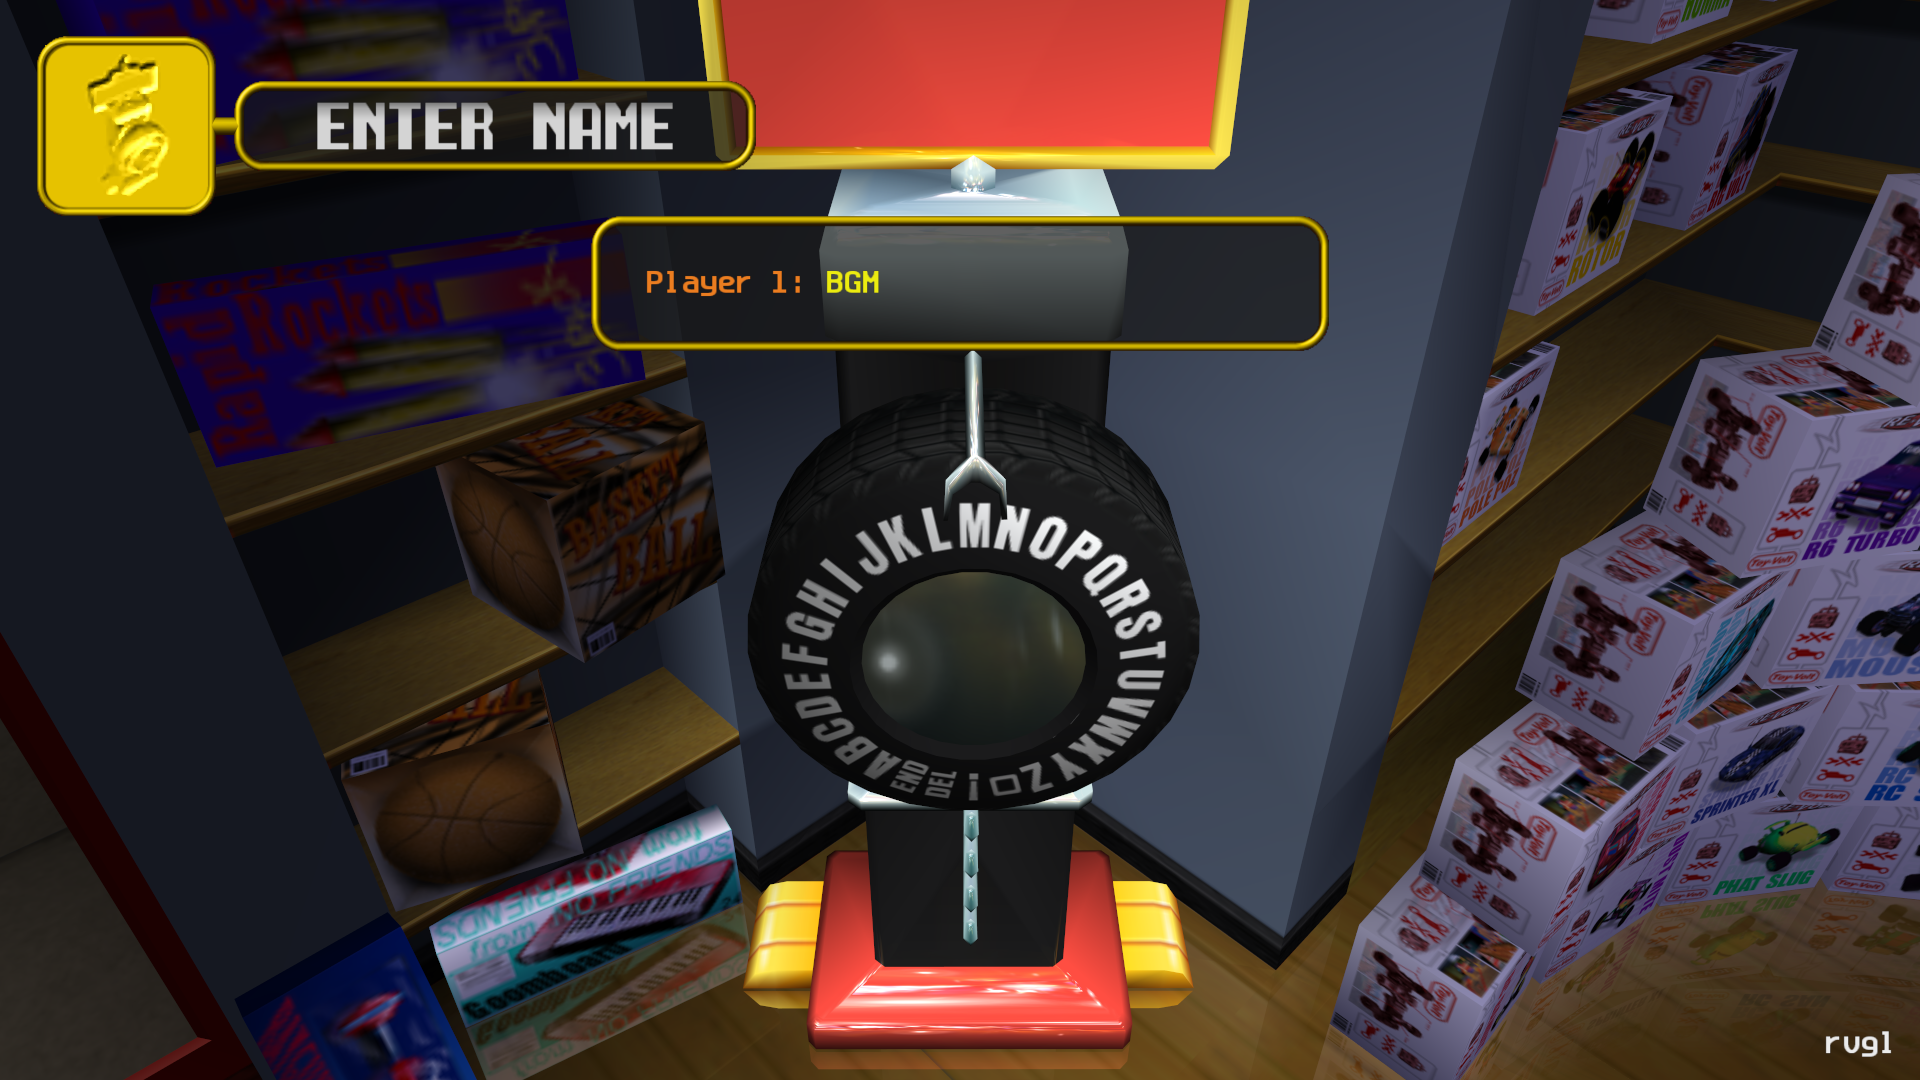
\includegraphics[width=15cm, height=8cm]{img/username.png}

\subsubsection{Autos y Categorías}
En Re-Volt, existen diferentes tipos de autos que pueden ser elegidos por el jugador. En el juego original, estos autos se clasifican en categorías según su velocidad máxima, aceleración, peso, y desempeño general en pista. Las categorías originales, ordenadas desde los autos más lentos, hasta los más rápidos, son las siguientes:

\begin{itemize}
	\item Rookie (Novato).
	\item Amateur (Amateur).
	\item Advanced (Avanzado).
	\item Semi-Pro (Semi-Profesional).
	\item Pro (Profesional).
\end{itemize}

Además de las categorías originales, también existen categorías especiales que han surgido a partir del contenido creado por la comunidad de Re-Volt y RVGL. Estas categorías son las siguientes:

\begin{itemize}
	\item Super-Pro
	\item Clockwork
\end{itemize}

La categoría o ''Rating'' de cada auto puede apreciarse desde el menú del juego, tal como se puede ver en la figura FIGNUM.

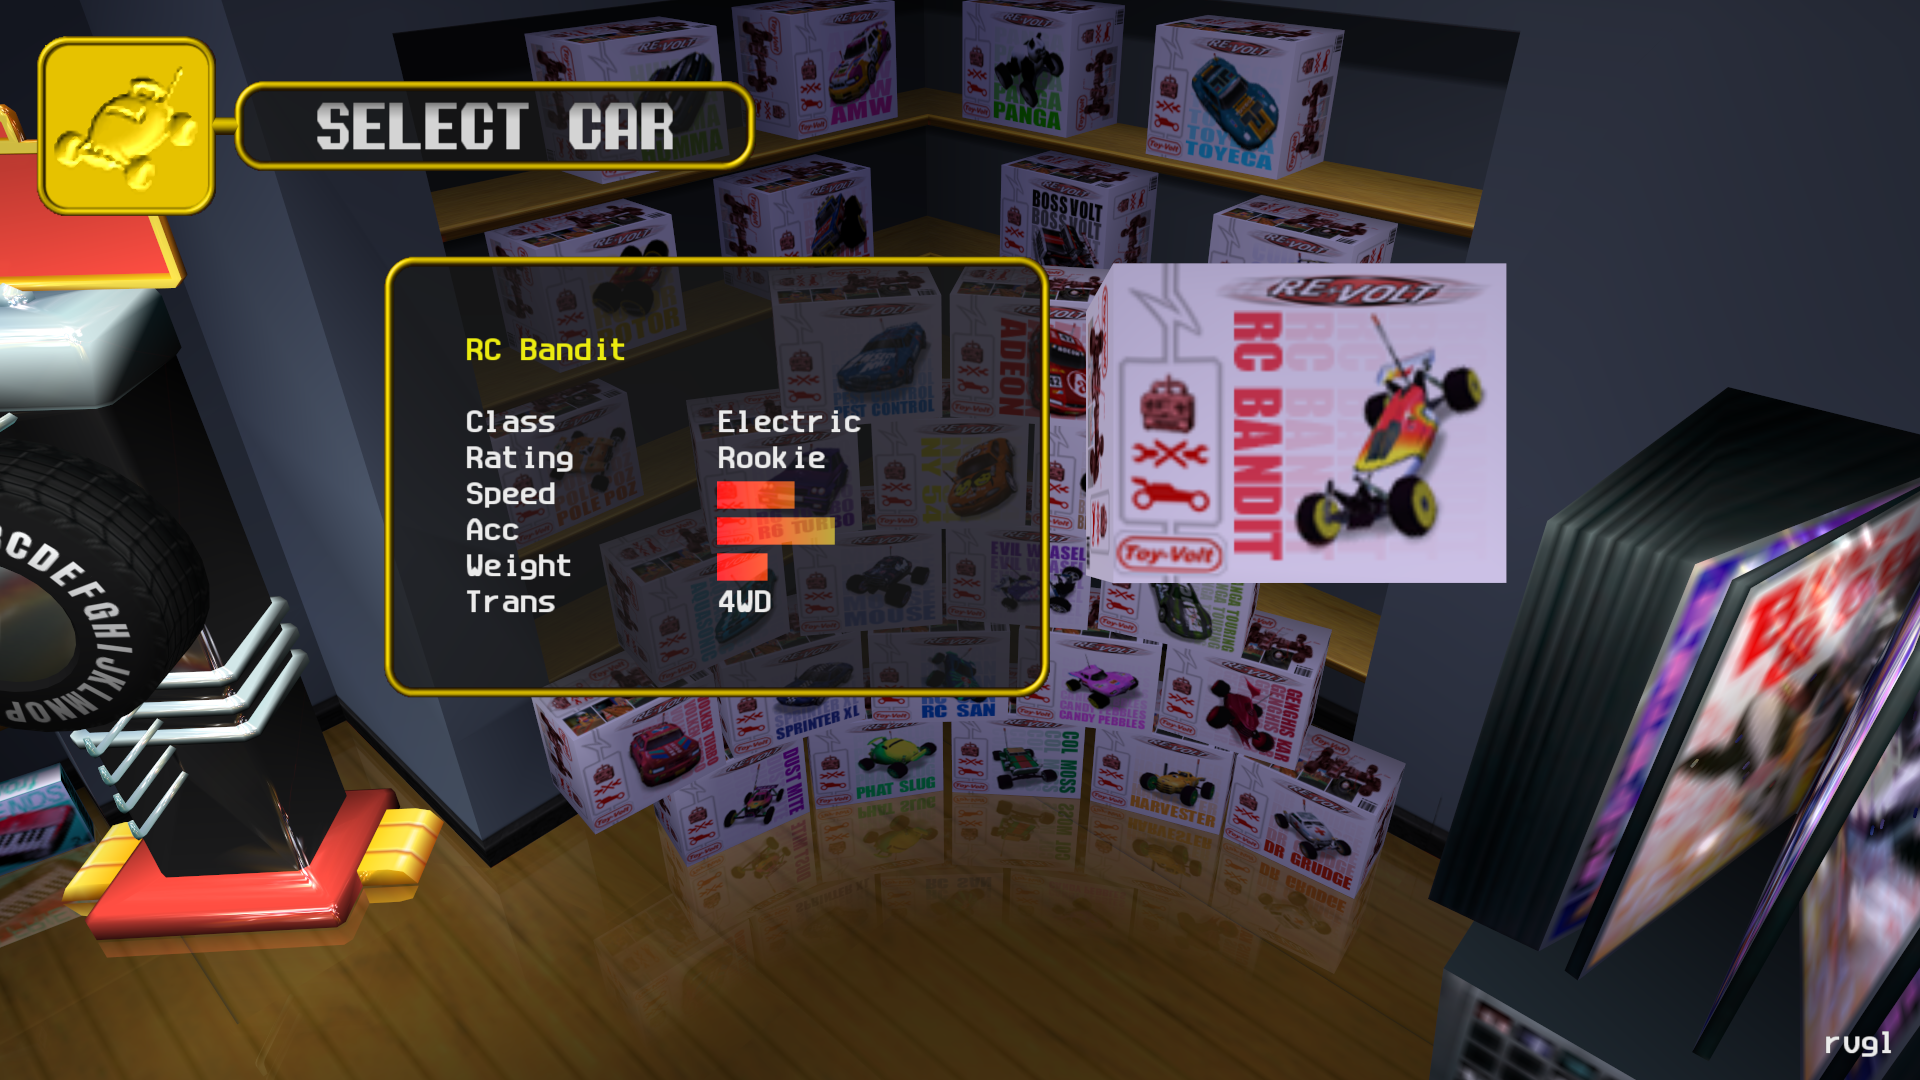
\includegraphics[width=15cm, height=8cm]{img/bandit.png}

De manera habitual, el anfitrión define una categoría de auto con la cual se jugará la sesión. De esta forma, todos los jugadores que se conecten deberán utilizar autos de la categoría definida.

Teniendo en cuenta lo anterior, las sesiones suelen ser nombradas a partir de su categoría asociada. Por ejemplo, si para una sesión se decide jugar autos de la categoría ''Pro'', es normal que esta sea titulada  ''Pros Session'', o ''Pro Races'' al momento de ser anunciada.

\subsubsection{Sala de Espera}
Una vez que el usuario elige su auto, este es llevado a la sala de espera, la cual viene representada por la figura FIGNUM.

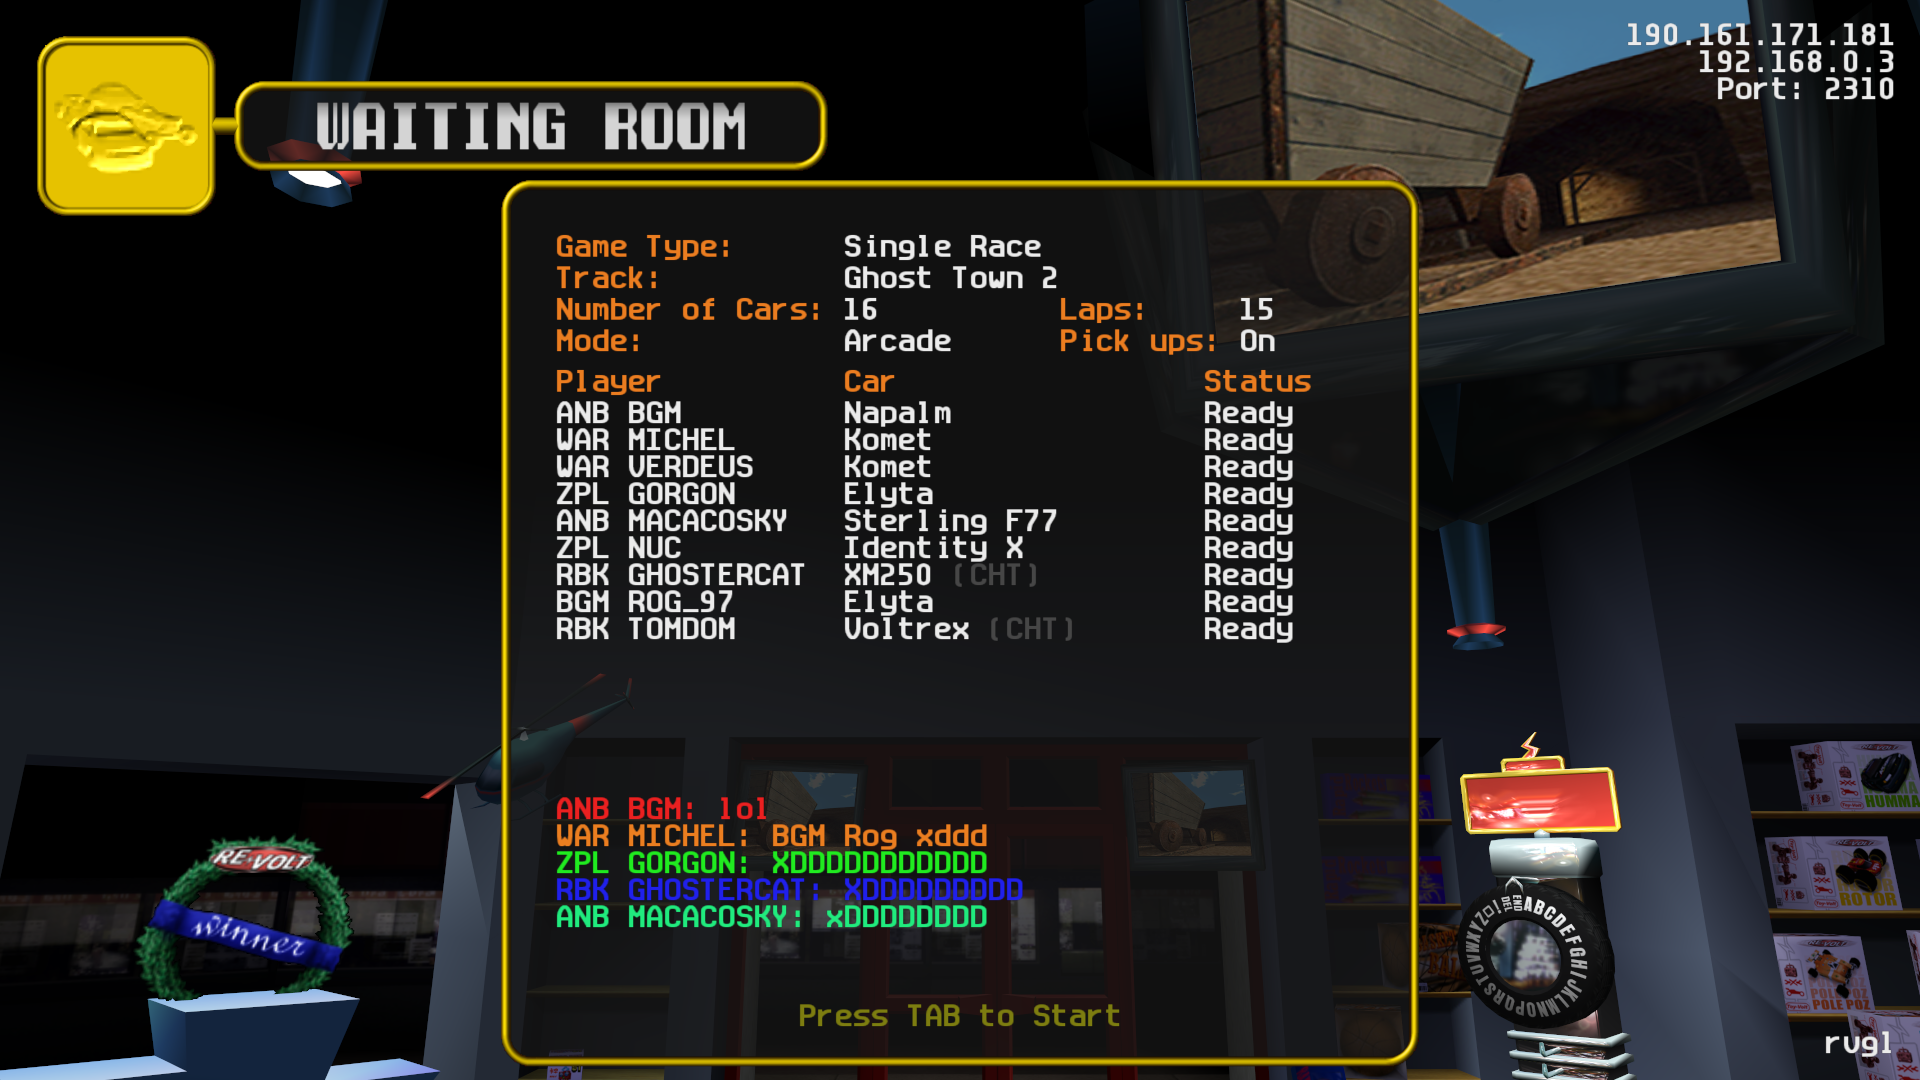
\includegraphics[width=15cm, height=8cm]{lobby.png}

Una vez llegados a este punto, sólo se debe esperar a que el anfitrión de la sesión de inicio a las carreras.

\subsubsection{Carreras en Línea}
Normalmente, en las partidas multijugador, suelen jugarse muchas carreras de manera consecutiva. A estas series de partidas en línea se les conoce como ''sesiones''. Cada sesión de Re-Volt consiste en una cantidad predefinida de carreras en pistas determinadas y con cierta clase de autos. Estas determinaciones las realiza el anfitrión de la partida, quien las comunica públicamente de manera oportuna para que todos aquellos que deseen participar tengan en cuenta todas las características de la sesión que van a jugar.

Las siguientes dos ilustraciones presentan las instancias clave dentro del juego. En la ilustración FIGNUM, se puede apreciar la perspectiva del jugador al momento de jugar Re-Volt. Luego, en la ilustración FIGNUM, se puede ver la tabla de resultados que se muestra por pantalla a medida que los corredores finalizan la carrera.

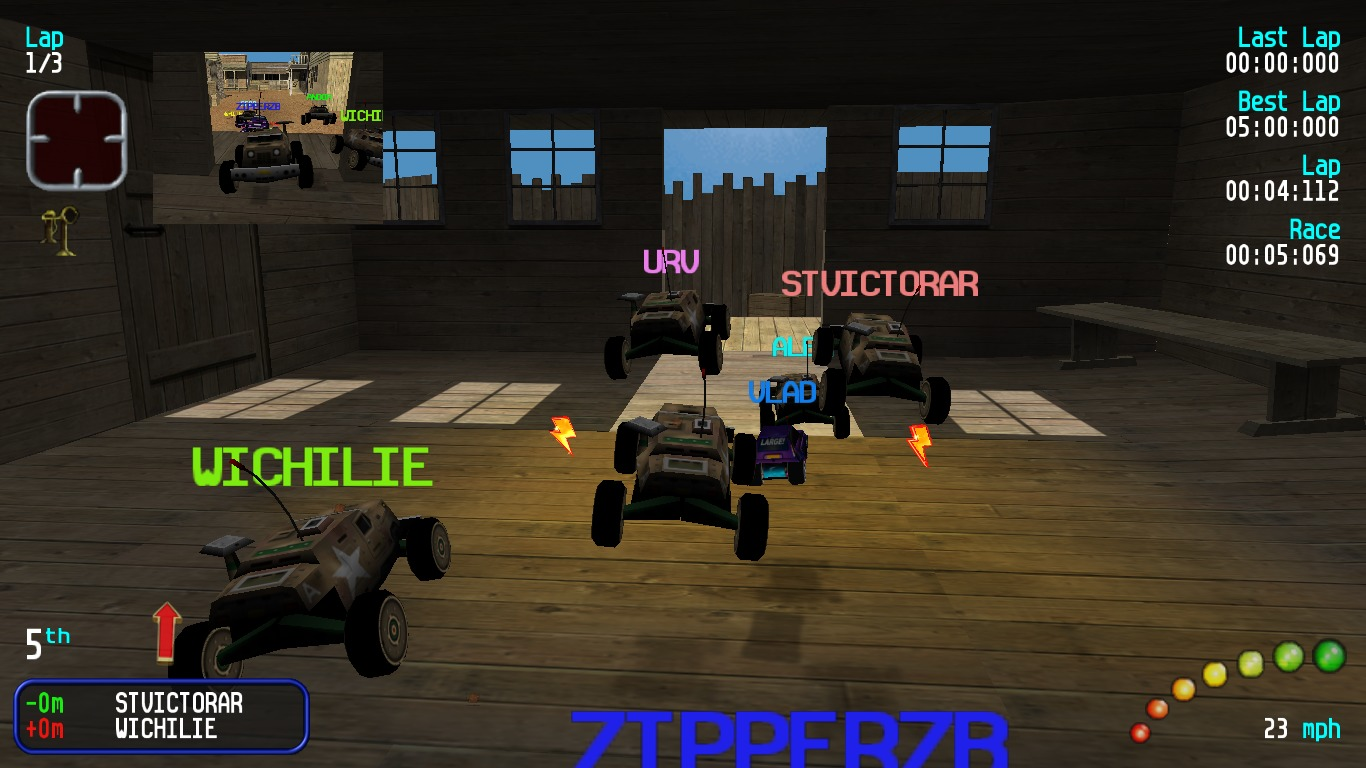
\includegraphics[width=15cm, height=8cm]{img/gameplay.jpg}

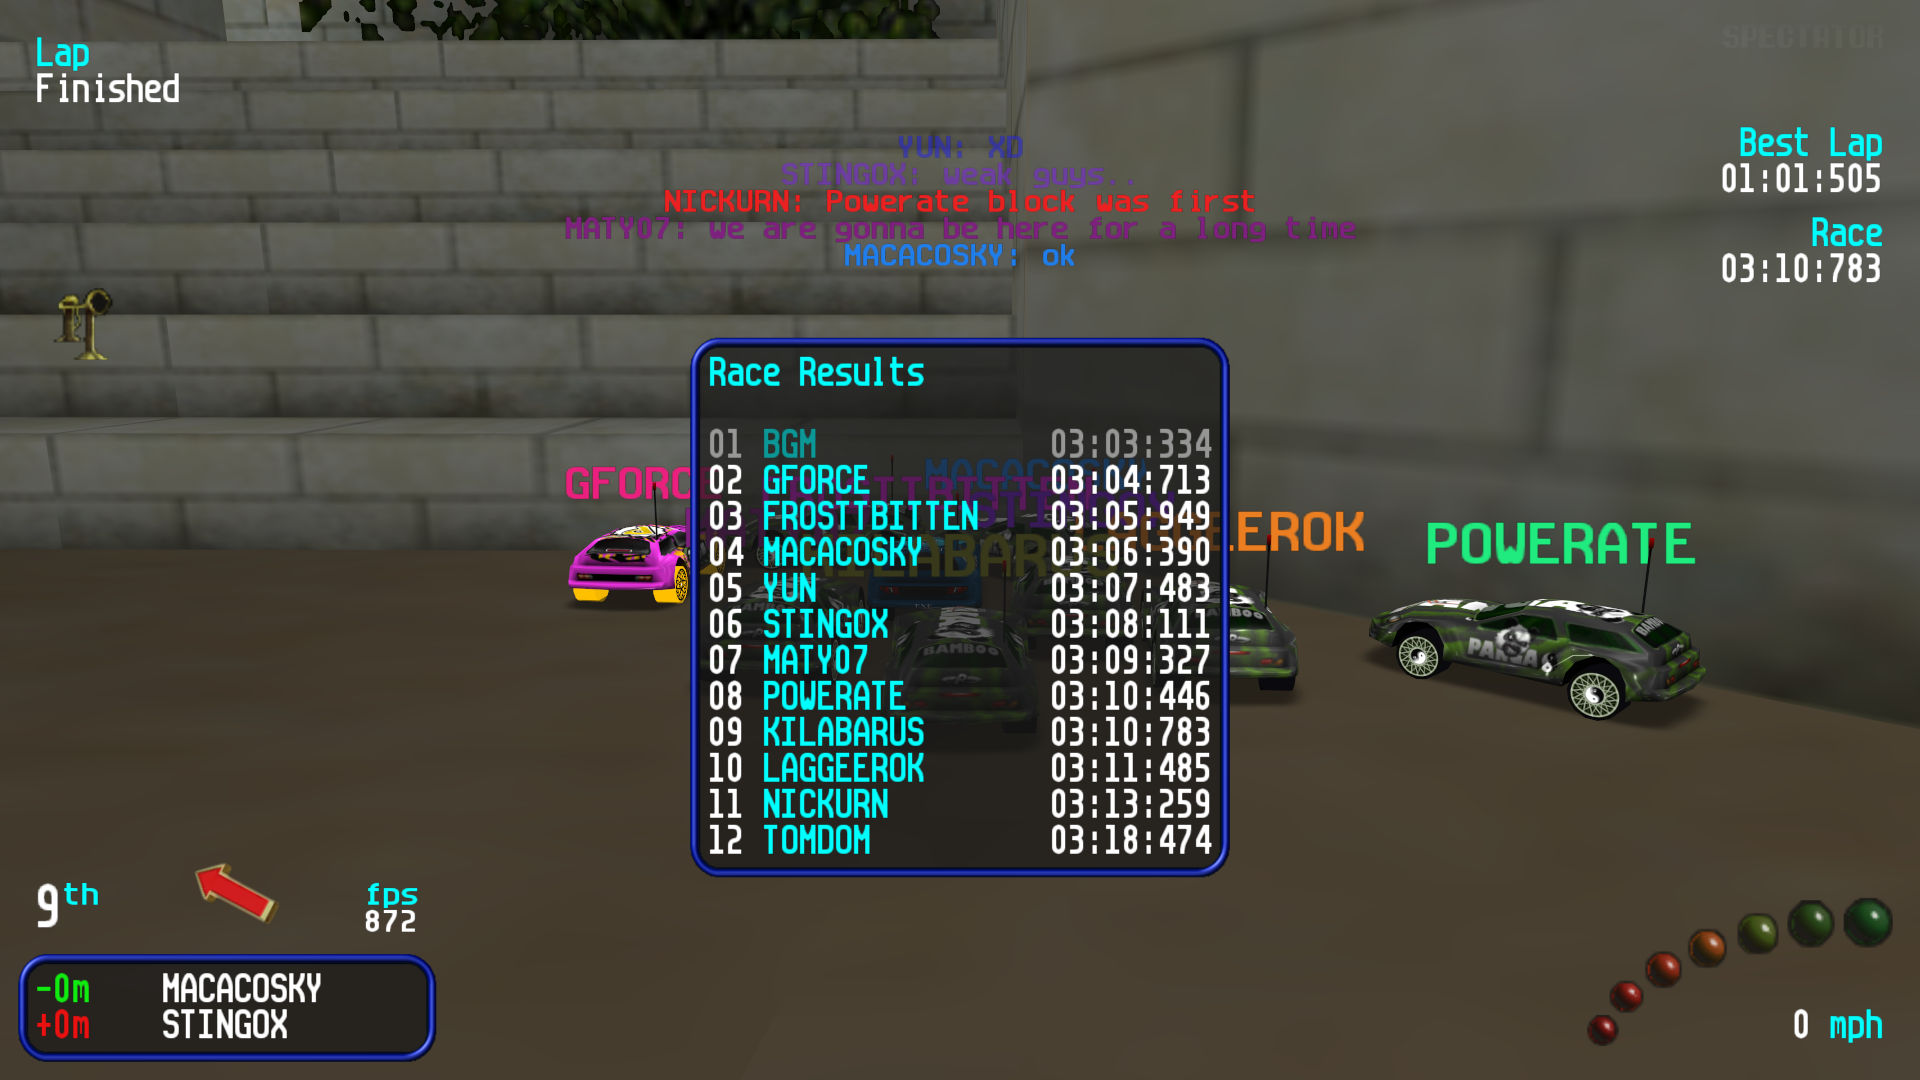
\includegraphics[width=15cm, height=8cm]{img/results.png}

\subsection{Re-Volt: OpenGL y los Session Logs}

Para ayudar a llevar una cuenta fiable de todas las carreras jugadas, RVGL introduce una funcionalidad que permite a los jugadores obtener un registro escrito de los resultados de cada carrera. Este registro viene en forma de un archivo separado por comas, el cual es conocido por la comunidad como Session Log. Este es el archivo que utilizan los organizadores y administradores de RVA para calcular los resultados oficiales de las sesiones.

En la ilustración FIGNUM, presentada a continuación, puede apreciarse un extracto del Session Log de una sesión cualquiera, el cual ha sido importado desde Microsoft Excel para una visualización más clara. Este extracto representa una sola de las carreras jugadas en la sesión. Entiéndase que, inmediatamente después de la última línea, vendría escrita la carrera siguiente, y así sucesivamente con todas las demás.

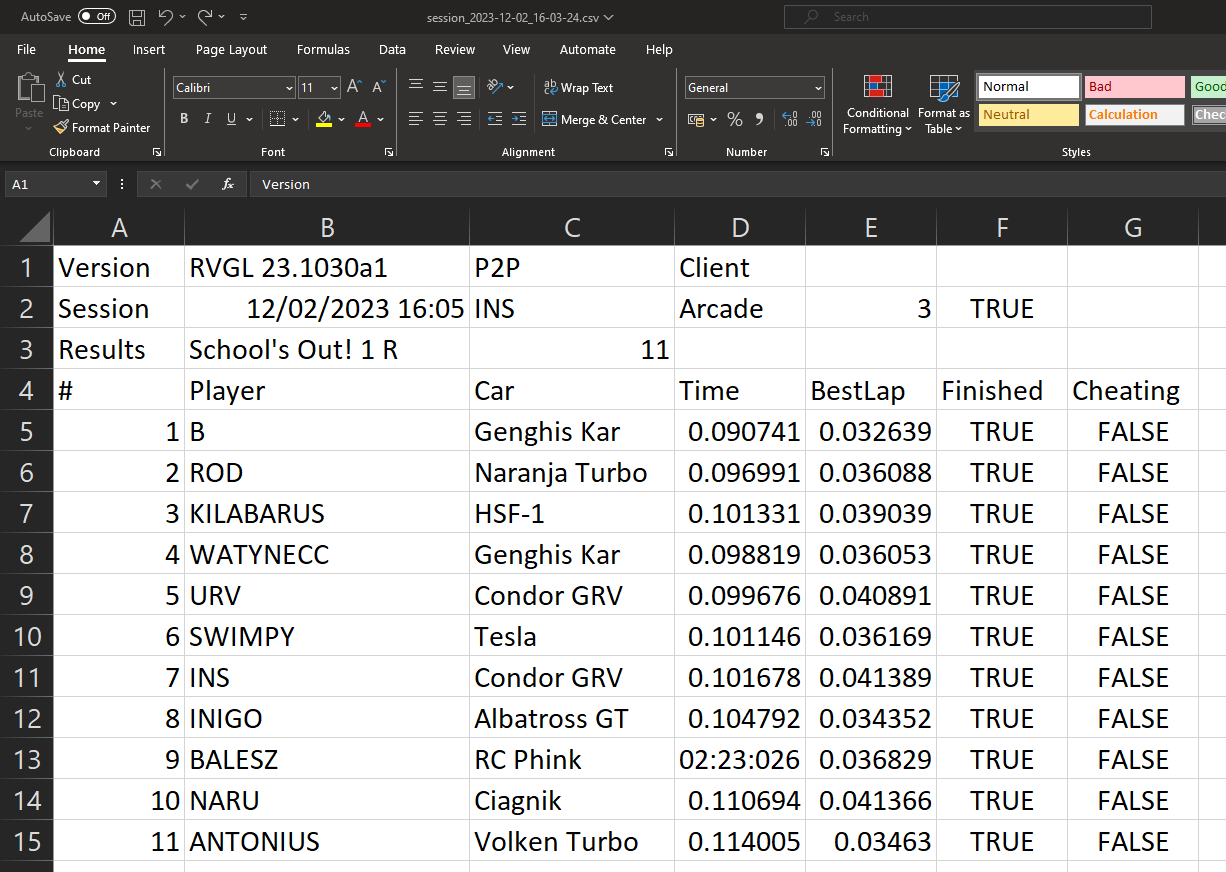
\includegraphics[width=16cm, height=14cm]{img/raw-results.png}

A continuación, la tabla TABLENUM es una especificación de los elementos relevantes de un Session Log. Algunos de dichos elementos son utilizados por RVA para calcular los resultados acumulados de las sesiones, para así obtener una tabla con posiciones finales para cada jugador al final de cada sesión.

\begin{center}
	\begin{tabular}{ | l | p{15cm} |}
		\hline
		\multicolumn{2}{|c|}{\textbf{Elementos de un Session Log}} \\
		\hline
		\multicolumn{1}{|c|}{\textbf{Id}} & \multicolumn{1}{|c|}{\textbf{Descripción}} \\
		\hline
		{\textbf{B1}} & Versión de RVGL de la sesión jugada. \\ \hline
		
		{\textbf{C1-D1}} & Protocolo de conexión de la sesión. \\ \hline
		
		{\textbf{B2}} & Fecha y hora de apertura de la sesión. \\ \hline
		
		{\textbf{C2}} & Nombres del jugador anfitrión de la sesión. \\ \hline
		
		{\textbf{D2}} & Tipo de colisión entre autos, seleccionado por el anfitrión. \\ \hline
		
		{\textbf{E2}} & Número de vueltas de esta carrera. \\ \hline
		
		{\textbf{B3}} & Nombre de la pista de esta carrera. \\ \hline
		
		{\textbf{C3}} & Número de jugadores que comenzaron la carrera. Si un jugador se desconecta en mitad de la carrera, este número no se ve afectado. \\ \hline
		
		{\textbf{B5-B15}} & Nombres de los jugadores que participaron de la carrera, agregados de arriba hacia abajo por orden de llegada a la línea de meta. \\ \hline
		
		{\textbf{C5-C15}} & Nombres de los autos utilizados por cada jugador en esta carrera. \\ \hline
		
		{\textbf{D5-D15}} & Tiempo total de la carrera de cada jugador.\\ \hline
		
		{\textbf{E5-E15}} & Mejor vuelta de cada jugador.\\ \hline
		
		{\textbf{F5-F15}} & TRUE si el jugador finalizó la carrera. FALSE si el jugador se desconectó en mitad de la carrera.\\ \hline
		
		{\textbf{G5-G15}} & TRUE si los archivos locales del jugador no corresponden a los archivos del anfitrión. FALSE si estos coinciden. Por ejemplo, ''Cheating'' es TRUE si un jugador modificó localmente la velocidad de su auto.\\ \hline
	\end{tabular}
\end{center}

\subsection{Funcionamiento Interno de Re-Volt America}

\subsubsection{Sistema de Temporadas, Rankings y Sesiones}
Históricamente, Re-Volt America se ha dedicado a organizar sesiones multijugador de Re-Volt para su público, así como también se ha preocupado de llevar la cuenta de los resultados de cada carrera que se ha jugado en ellas. Esto lo hace mediante un sistema de temporadas.

Todos los jugadores que, en algún momento u otro, han participado en las sesiones online organizadas por Re-Volt America, han sido indexados en la base de datos de jugadores que mantiene la comunidad. De esta forma, sus victorias, puntos y otras estadísticas asociadas han sido preservadas a lo largo del tiempo.

Para conseguir un sistema atractivo para sus jugadores, Re-Volt America organiza sus sesiones en una serie de rankings, los cuales consisten en 28 sesiones multijugador cada uno, jugandose una sesión al día. Al cumplirse 6 de estos rankings, se completa lo que en RVA se conoce como una temporada.

Cada sesión organizada por RVA consiste en 20 carreras, las cuales se juegan en 20 pistas diferentes. Es por esto que, en una sesión, se producen 20 sets de resultados (1 por carrera).

Cada año, en promedio, se inician dos temporadas, y cada una es nombrada en base a su año de inicio, y su periodo en relación a otras temporadas. Por ejemplo, si en el año 2023 se da inicio a una temporada en el mes de enero, esta vendría a llamarse ''2023'', ya que terminará dentro del mismo año en el que inició. Por otra parte, si la temporada inicia en el mes de diciembre de 2023, esto quiere decir que terminará dentro del año 2024, por lo que pasaría a llamarse ''2023-24''.

Es así como Re-Volt America, desde el año 2017, hasta el presente, ha conseguido consolidarse como la comunidad de Re-Volt predilecta para los jugadores tanto de norteamerica como América latina.

\subsubsection{Paquete de Contenido de RVA}
Re-Volt America cuenta con un paquete de contenido extra para RVGL, el cual es construido por sus administradores y organizadores al principio de cada temporada.

Este paquete consiste en una selección de autos y pistas para RVGL hechos por la comunidad, los cuales tienen el objetivo de extender el contenido original del juego, y así proveer a los usuarios con una experiencia más enriquecedora y variada al momento de jugar en línea.

El paquete de contenido de RVA, más conocido como RVA Pack, es, técnicamente, un conjunto de archivos correspondientes a los autos y pistas que este busca agregar. Estos archivos son mandatorios para poder participar de las sesiones organizadas por RVA. Esto quiere decir que, para que un usuario pueda entrar a una sesión de RVA, este debe tener instalado el RVA Pack en su instalación de RVGL local.

\subsubsection{Sistema de Puntuación}
Como se ha aludido a lo largo del estudio del problema, la comunidad de Re-Volt America cuenta con su propio sistema de puntuación, el cual le sirve para generar estadísticas por jugador, tablas de resultados al final de cada sesión, y demás métricas que, finalmente, promueven la competitividad y enriquecen la experiencia de los usuarios.

El funcionamiento de dicho sistema de puntuación es el siguiente: dependiendo de la posición da cada jugador, al final de cada carrera, a estos se les asigna un puntaje. El mapeo de puntos para una carrera con menos de 10 participantes viene definido por la siguiente función que relaciona posiciones con puntos, respectivamente:

\newpage

\[\hspace*{1.2cm} pos \hspace*{0.3cm} f_1(pos)\]
\[
\mathlarger{
	f_1= 
	\begin{cases}
		1 \to 15 \\
		2 \to 12 \\
		3 \to 10 \\
		4 \to 7 \\
		5 \to 5 \\
		6 \to 4 \\
		7 \to 2 \\
		8 \to 2 \\
		9 \to 1
	\end{cases}
}
\]

Por otro lado, en caso de que la carrera cuente con 10 jugadores o más, el mapeo de puntos sería el siguiente:

\[\hspace*{1.2cm} pos \hspace*{0.3cm} f_2(pos)\]
\[
\mathlarger{
	f_2= 
	\begin{cases}
		1 \to 20 \\
		2 \to 16 \\
		3 \to 12 \\
		4 \to 10 \\
		5 \to 8 \\
		6 \to 8 \\
		7 \to 6 \\
		8 \to 4 \\
		9 \to 2 \\
		10 \to 2 \\
		11 \to 1 \\
		12 \to 1 \\
		13 \to 1 \\
		14 \to 1 \\
		15 \to 1 \\
		16 \to 1
	\end{cases}
}
\]

Por lo tanto, el conjunto que define los posibles puntajes obtenibles viene definido de la siguiente manera:

\[
\mathlarger{
	P = \{1, 2, 4, 5, 6, 7, 8, 10, 12, 15, 16, 20\}
}
\]

Si se tiene que ''\textit{n}'' es la cantidad de jugadores que participaron de una carrera, entonces:

\[
\mathlarger{
	A = \{1, \dots, n\} \subset \mathbb{N}
}
\]

\[
\mathlarger{
	n = \lvert A \rvert
}
\]

Teniendo en cuenta lo anterior, es posible definir una función que, al recibir una posición final de un jugador en una carrera determinada, retorne la cantidad de puntos correspondientes a dicha posición. Esta función vendría definida a continuación, en donde ''\textit{pos}'' es la posición final del jugador en la carrera en cuestión.

\[
\mathlarger{
f : pos \in A \to 
\begin{cases}
	f_1(pos) & \text{if } n < 10\\
	f_2(pos) & \text{if } n \geq 10
\end{cases}
\in P
}
\]

Al finalizar una sesión, todos los puntajes de cada jugador, obtenidos en cada carrera, son sumados, normalizados, y sometidos a diferentes procesos de ajuste propios del sistema de RVA. Una vez ajustados, estos pasarán a ser los puntajes finales de la sesión.


\subsubsection{Cálculo de Resultados}
Una vez procesados, los resultados son llevados a una tabla final, tal como se puede apreciar en la figura FIGNUM.

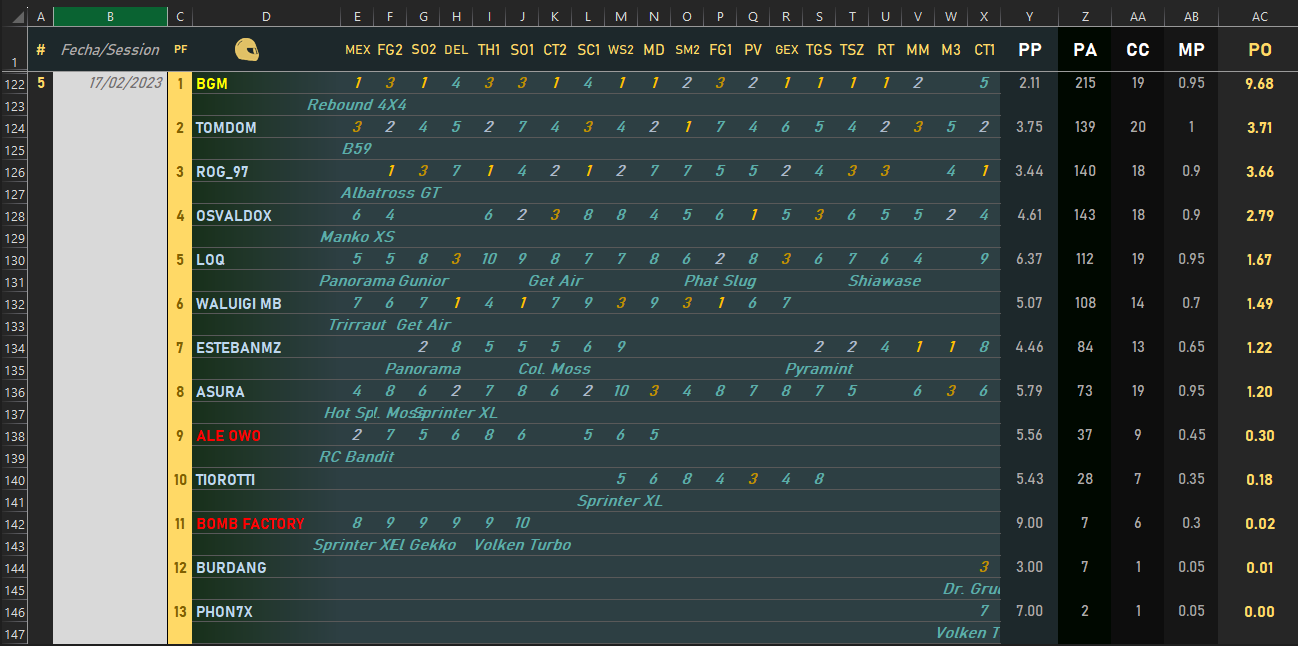
\includegraphics[width=15cm, height=10cm]{old-results.png}

\begin{center}
	\begin{tabular}{ | p{5cm} | l | p{8cm} |}
		\hline
		\multicolumn{3}{|c|}{\textbf{Parámetros}} \\
		\hline
		\multicolumn{1}{|c|}{\textbf{Nombre}} & \multicolumn{1}{|c|}{\textbf{Abreviación}} & \multicolumn{1}{|c|}{\textbf{Descripción}} \\
		\hline
		{\textbf{Posición Promedio}} & PP & La suma de las posiciones del jugador, dividida por su cantidad de carreras corridas. \\ \hline
		{\textbf{Puntaje Acumulado}} & PA & La suma total de los puntos correspondientes a las posiciones obtenidas por el jugador. \\ \hline
		{\textbf{Carreras Corridas}} & CC & La cantidad de carreras corridas por el jugador. \\ \hline
		{\textbf{Multiplicador por Participación}} & MP & La cantidad de carreras corridas por el jugador, divida por la cantidad de carreras totales de la sesión. \\ \hline
		{\textbf{Puntaje Oficial}} & PO & El puntaje acumulado del jugador, multiplicado por un factor normalizador de 0.1. \\ \hline
	\end{tabular}
\end{center}


De acuerdo con la tabla anterior, los cálculos de PA, PP y MP pueden ser representados utilizando las siguientes fórmulas, respectivamente, en donde ''\textit{pos}'' es la posición del jugador en cada carrera, y ''\textit{tot}'' la cantidad total de carreras de la sesión.

\[
\mathlarger{{PA} = \sum_{i=1}^{CC}x=x+f(pos_i)}
\]

\[
\mathlarger{{PP} = \frac{\left(\sum\limits_{i=1}^{CC}x=x+pos_i\right)}{CC}}
\]

\[
\mathlarger{{MP} = \frac{CC}{tot}}
\]

A partir de estos parámetros, podemos calcular el puntaje oficial, o PO, obtenido por el jugador en la sesión en cuestión.

\[
\mathlarger{{PO} = \left(\frac{PA}{PP} \cdot MP\right) \cdot 0.1}
\]

\subsubsection{Multiplicadores por Auto}
Como ya se mencionó anteriormente, al principio de cada temporada, se agregan y se eliminan autos del pack de RVA. Asimismo, RVA introduce el concepto de multiplicadores para dichos autos por temporada.

De acuerdo con el sistema de RVA, el puntaje obtenido por un jugador al finalizar una carrera es multiplicado por el multiplicador del auto que utiliza en dicha carrera. De esta forma, el puntaje obtenido por el jugador incrementa o disminuye dependiendo del multiplicador asociado a su auto.

Los multiplicadores de cada auto son un reflejo de su potencial para desempeñarse en carreras en línea en comparación a los demás autos de su categoría. Por ejemplo, si un auto es increíblemente rápido, fácil de manejar y no tiene dificultad alguna, entonces este se le asocia con un multiplicador bajo, para así nivelar los puntos que, potencialmente, pueda obtener un jugador al utilizarlo. Por el contrario, si un auto es muy lento, difícil de manejar, y simplemente es peor que los demás autos de su categoría, entonces se le asocia con un multiplicador alto, para así otorgar puntos extra a quien lo utilice.

La decisión de qué autos son buenos y qué autos son malos, en comparación con los demás de su categoría, es tomada por la administración de RVA en base a pruebas de manejo para los autos, y la experiencia previa en temporadas anteriores. A partir de esta decisión, se le otorga un multiplicador a cada auto.

Considerando los distintos multiplicadores que puede tener cada auto, la fórmula para el cálculo del PA es modificada ligeramente, en donde ''\textit{mul}'' es el multiplicador del auto asociado.

\[
\mathlarger{{PA} = \sum_{i=1}^{CC}x=x+f(pos_i) \cdot mul_i}
\]

Como se explicó anteriormente, existen varias categorías de autos en Re-Volt. Si bien las sesiones de RVA corresponden a una categoría a la vez, el sistema admite que jugadores elijan autos hasta 3 clases por debajo de la categoría de la sesión. Por ejemplo, si la sesión es publicada como de categoría ''Pro'', un jugador puede elegir un auto de categoría ''Semi-Pro''.

De acuerdo con el sistema de RVA, por cada categoría de diferencia entre la sesión y el auto elegido por el jugador, a este se le otorga un bono de 0.25, el cual se adiciona al multiplicador de su auto. Si en el ejemplo anterior la sesión era ''Pro'' y el auto ''Semi-Pro'', entonces al multiplicador del auto se le suma directamente 0.25. Si la diferencia fuese de 2 categorías, entonces se le sumaría 0.5.

Teniendo en cuenta lo anterior, la fórmula es modificada nuevamente. En este caso, la variable ''\textit{delta}'' representa el bono asignado al jugador en la carrera.

\[
\mathlarger{{PA} = \sum_{i=1}^{CC}x=x+f(pos_i) \cdot \left(mul_i + delta_i\right)}
\]

\section{Problemática Actual}
Hoy en día,  RVA utiliza una aplicación llamada ''RVA-Points'', la cual está hecha exclusivamente para procesar los Session Logs generados por RVGL y transformarlos en archivos separados por comas que contienen los resultados de las sesiones en el formato de RVA.

Una vez procesados los Session Logs, RVA lleva la cuenta de sus temporadas y jugadores utilizando Microsoft Excel como una pseudo base de datos para registrarlos, y Dropbox para la sincronización de archivos entre administradores.

Cada temporada, los administradores manejan un documento maestro de Excel, el cual, en resumidas cuentas, es utilizado para registrar los resultados de cada sesión y, a la vez, llevar la cuenta de los puntos por jugador. Esto se consigue utilizando macros y demás componentes característicos de Excel.

Los documentos relacionados a cada temporada son archivados utilizando una carpeta compartida en Dropbox.

Actualmente, el proceso diario para calcular y publicar los resultados de cada sesión es llevado a cabo, de manera semiautomática, por los administradores de RVA. Este proceso consiste en los siguientes pasos:

\begin{enumerate}
	\item Una vez finalizada la sesión, se busca el Session Log generado por RVGL, y este llega a los administradores de RVA.
	\item Se revisan los nombres de usuario manualmente. Esto se hace en caso de que algún jugador haya utilizado un nombre ligeramente distinto al que usa normalmente.
	\item El Session Log de la sesión es importado desde ''RVA-Points''. Este programa procesa el Session Log, y lo transforma en resultados ordenados en el formato de RVA.
	\item También desde ''RVA-Points'', los resultados procesados son exportados a otro archivo separado por comas.
	\item Se copian los contenidos del archivo exportado al documento maestro de la temporada actual.
	\item Se agrega cierta información de manera manual, como la fecha y número de la sesión.
	\item Se revisa manualmente que los nombres de usuario de la sesión correspondan a los nombres que ya figuran en el documento maestro.
	\item Se publica una fotografía de la tabla de resultados de la sesión en el Discord de RVA.
	\item Se publica una fotografía del ranking actualizado con los datos de la sesión en el Discord de RVA.
\end{enumerate}

A raíz de este largo y tedioso proceso de cálculo y manejo de resultados, se ha dado origen a este proyecto de título, como una oportunidad de mejorar dicho proceso, y poder ofrecer así una mejor experiencia de usuario tanto para los jugadores de RVA, como para los organizadores de la comunidad, quienes dedican su tiempo y esfuerzo a mantener estos registros históricos al día para todos.

\subsection{Diagrama de la Situación en la Actualidad}
Teniendo en cuenta el contexto del problema, la situación en la actualidad puede representarse a través del siguiente diagrama BPMN:
\begin{center}
	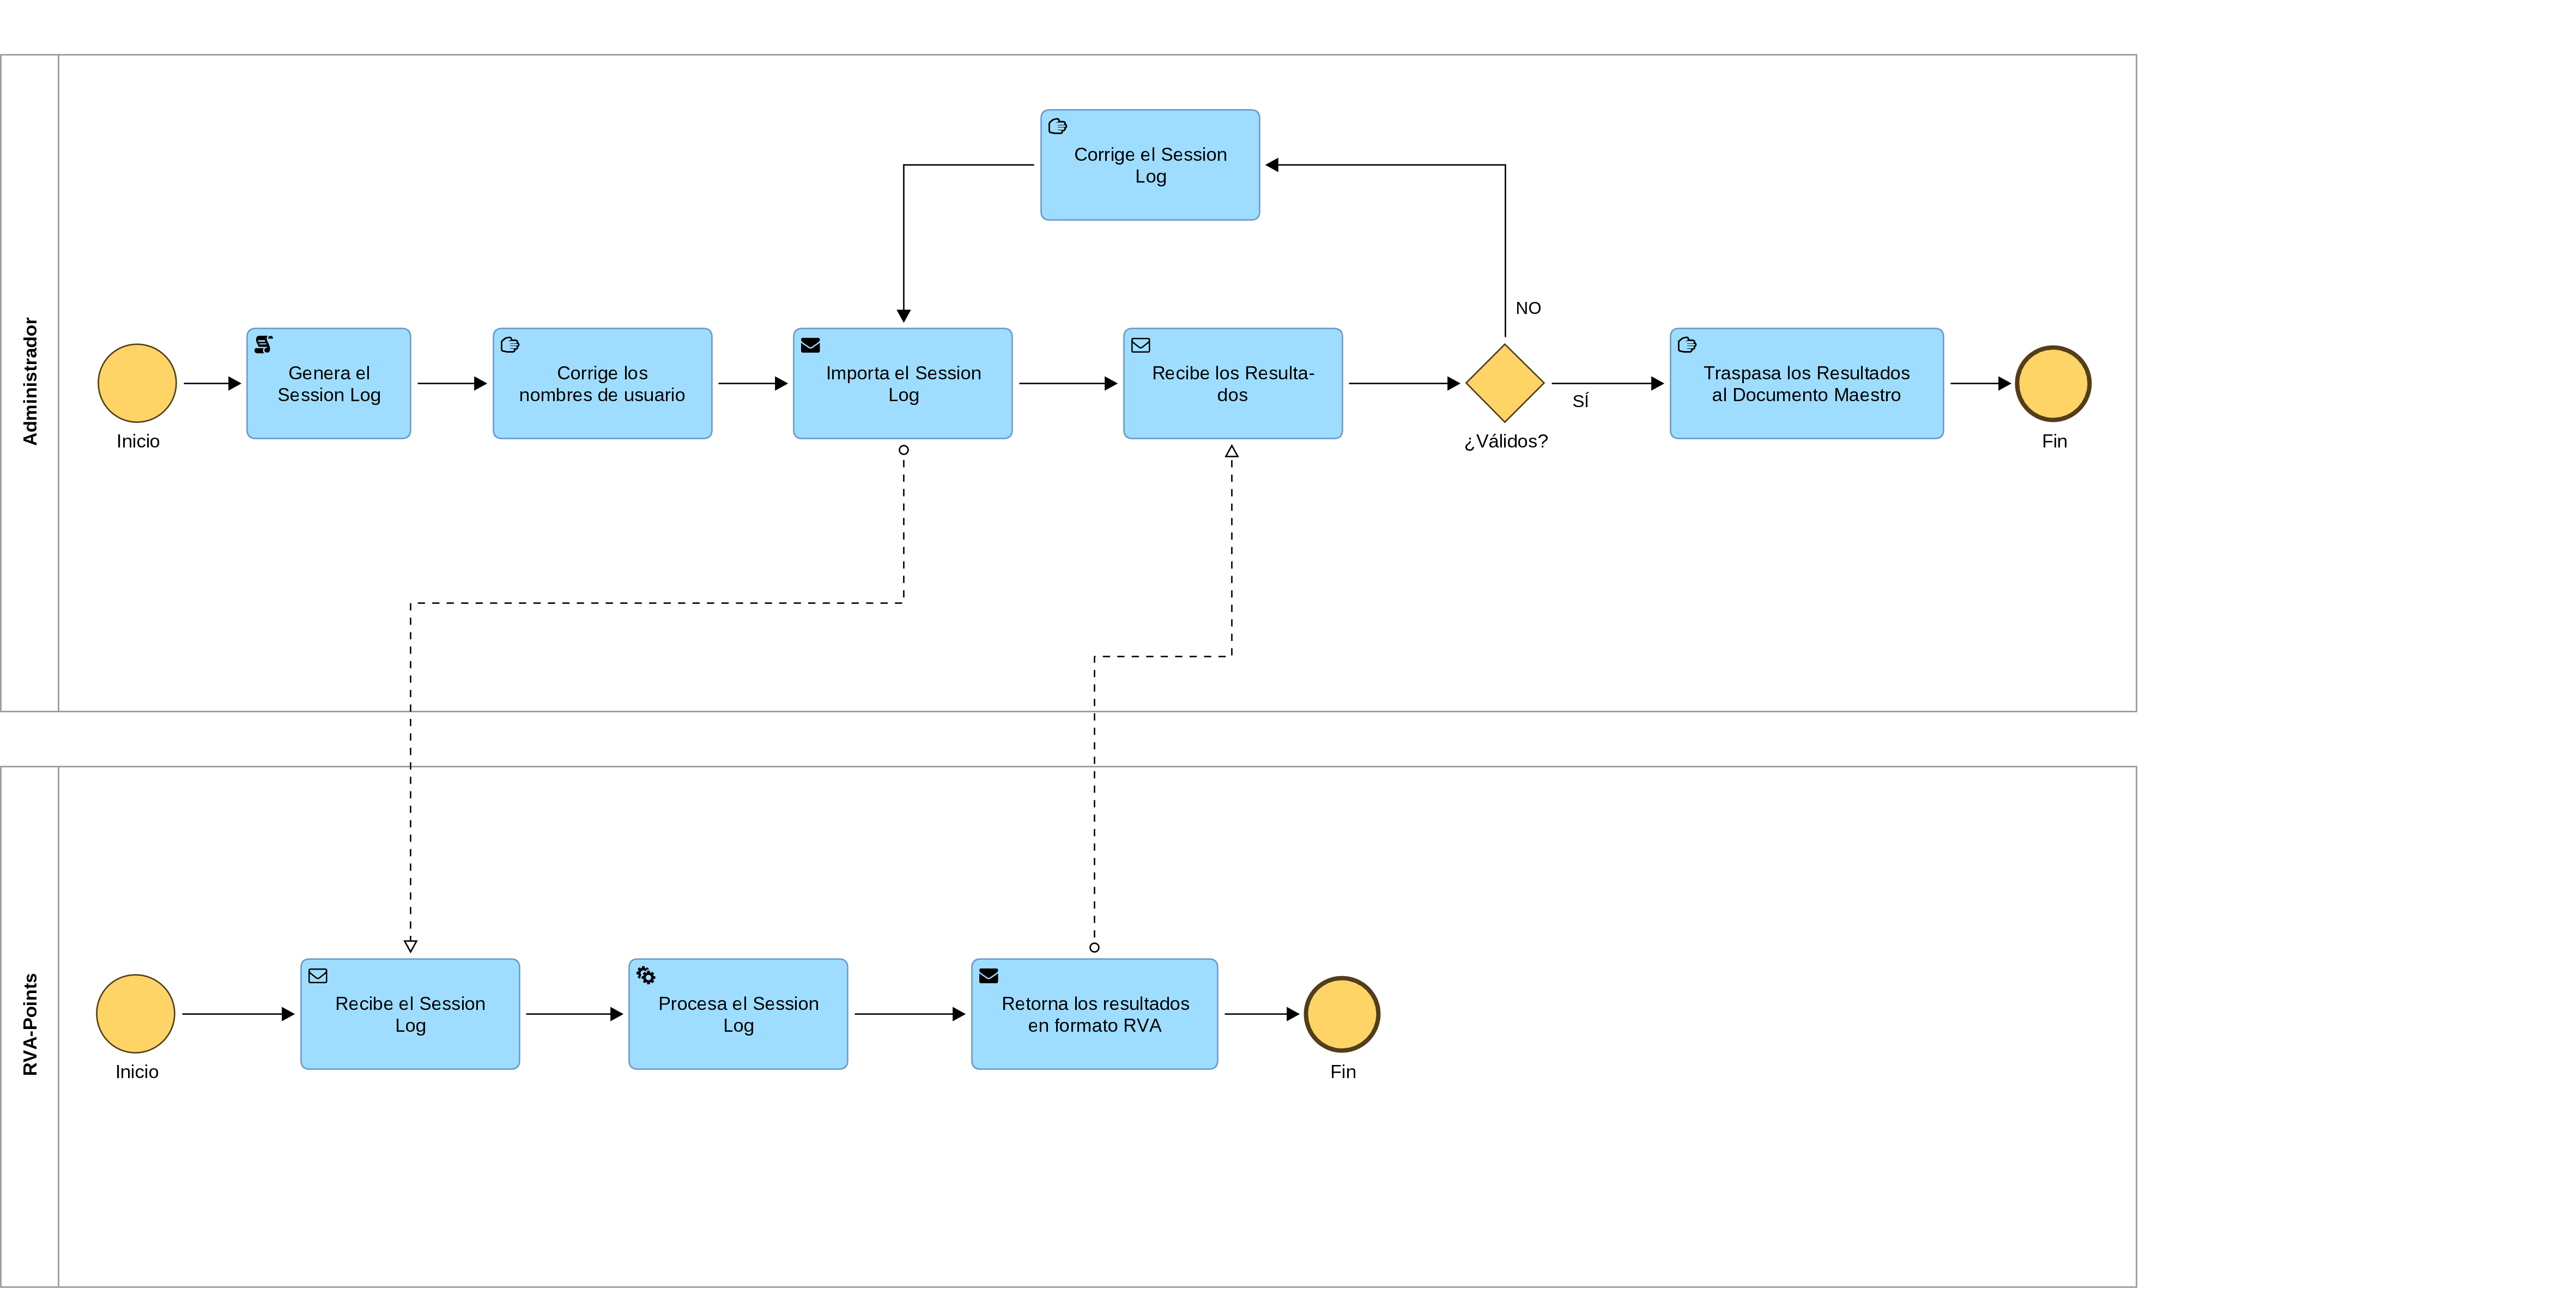
\includegraphics[width=21cm, height=12cm]{bpmn1.png}
\end{center}


\section{Propuesta de solución}
Debe explicar en términos generales cómo las TIC pueden resolver o mejorar la(s) problemática identificada y quienes serán los usuarios principales, que tecnología se utilizaría para dar soporte a la propuesta.

\section{Soluciones similares disponibles}
A continuación, se describen las soluciones disponibles que pueden ser catalogadas como similares al proyecto que se presenta.

\subsection{Aplicación para Cálculo de Puntos de Re-Volt I/O}
Existe un trabajo similar hace varios años, el cual fue desarrollado por la comunidad europea de RVGL: Re-Volt I/O.

Este trabajo se trata de una aplicación web que permite a los administradores de Re-Volt I/O importar los resultados de las sesiones multijugador, y poder visualizarlos dentro de la misma página; sin embargo, dicho proyecto no cuenta con ningún tipo de interconexión entre resultados, lo que quiere decir que cada sesión de carreras publicada en dicho sitio es independiente de otras. Debido a lo anterior, este proyecto no cuenta con perfiles de usuario, y por ende no permite visualizar estadísticas de ningún tipo, ni tampoco relacionar tablas de resultados entre si.

En general, esta solución fue concebida para ser algo simple y rápido que sirviera para calcular y renderizar resultados de manera oportuna, y no con una visión de persistencia en mente. A continuación, en la ilustración FIGNUM, puede apreciarse la tabla de resultados generada por la aplicación web de Re-Volt: I/O.

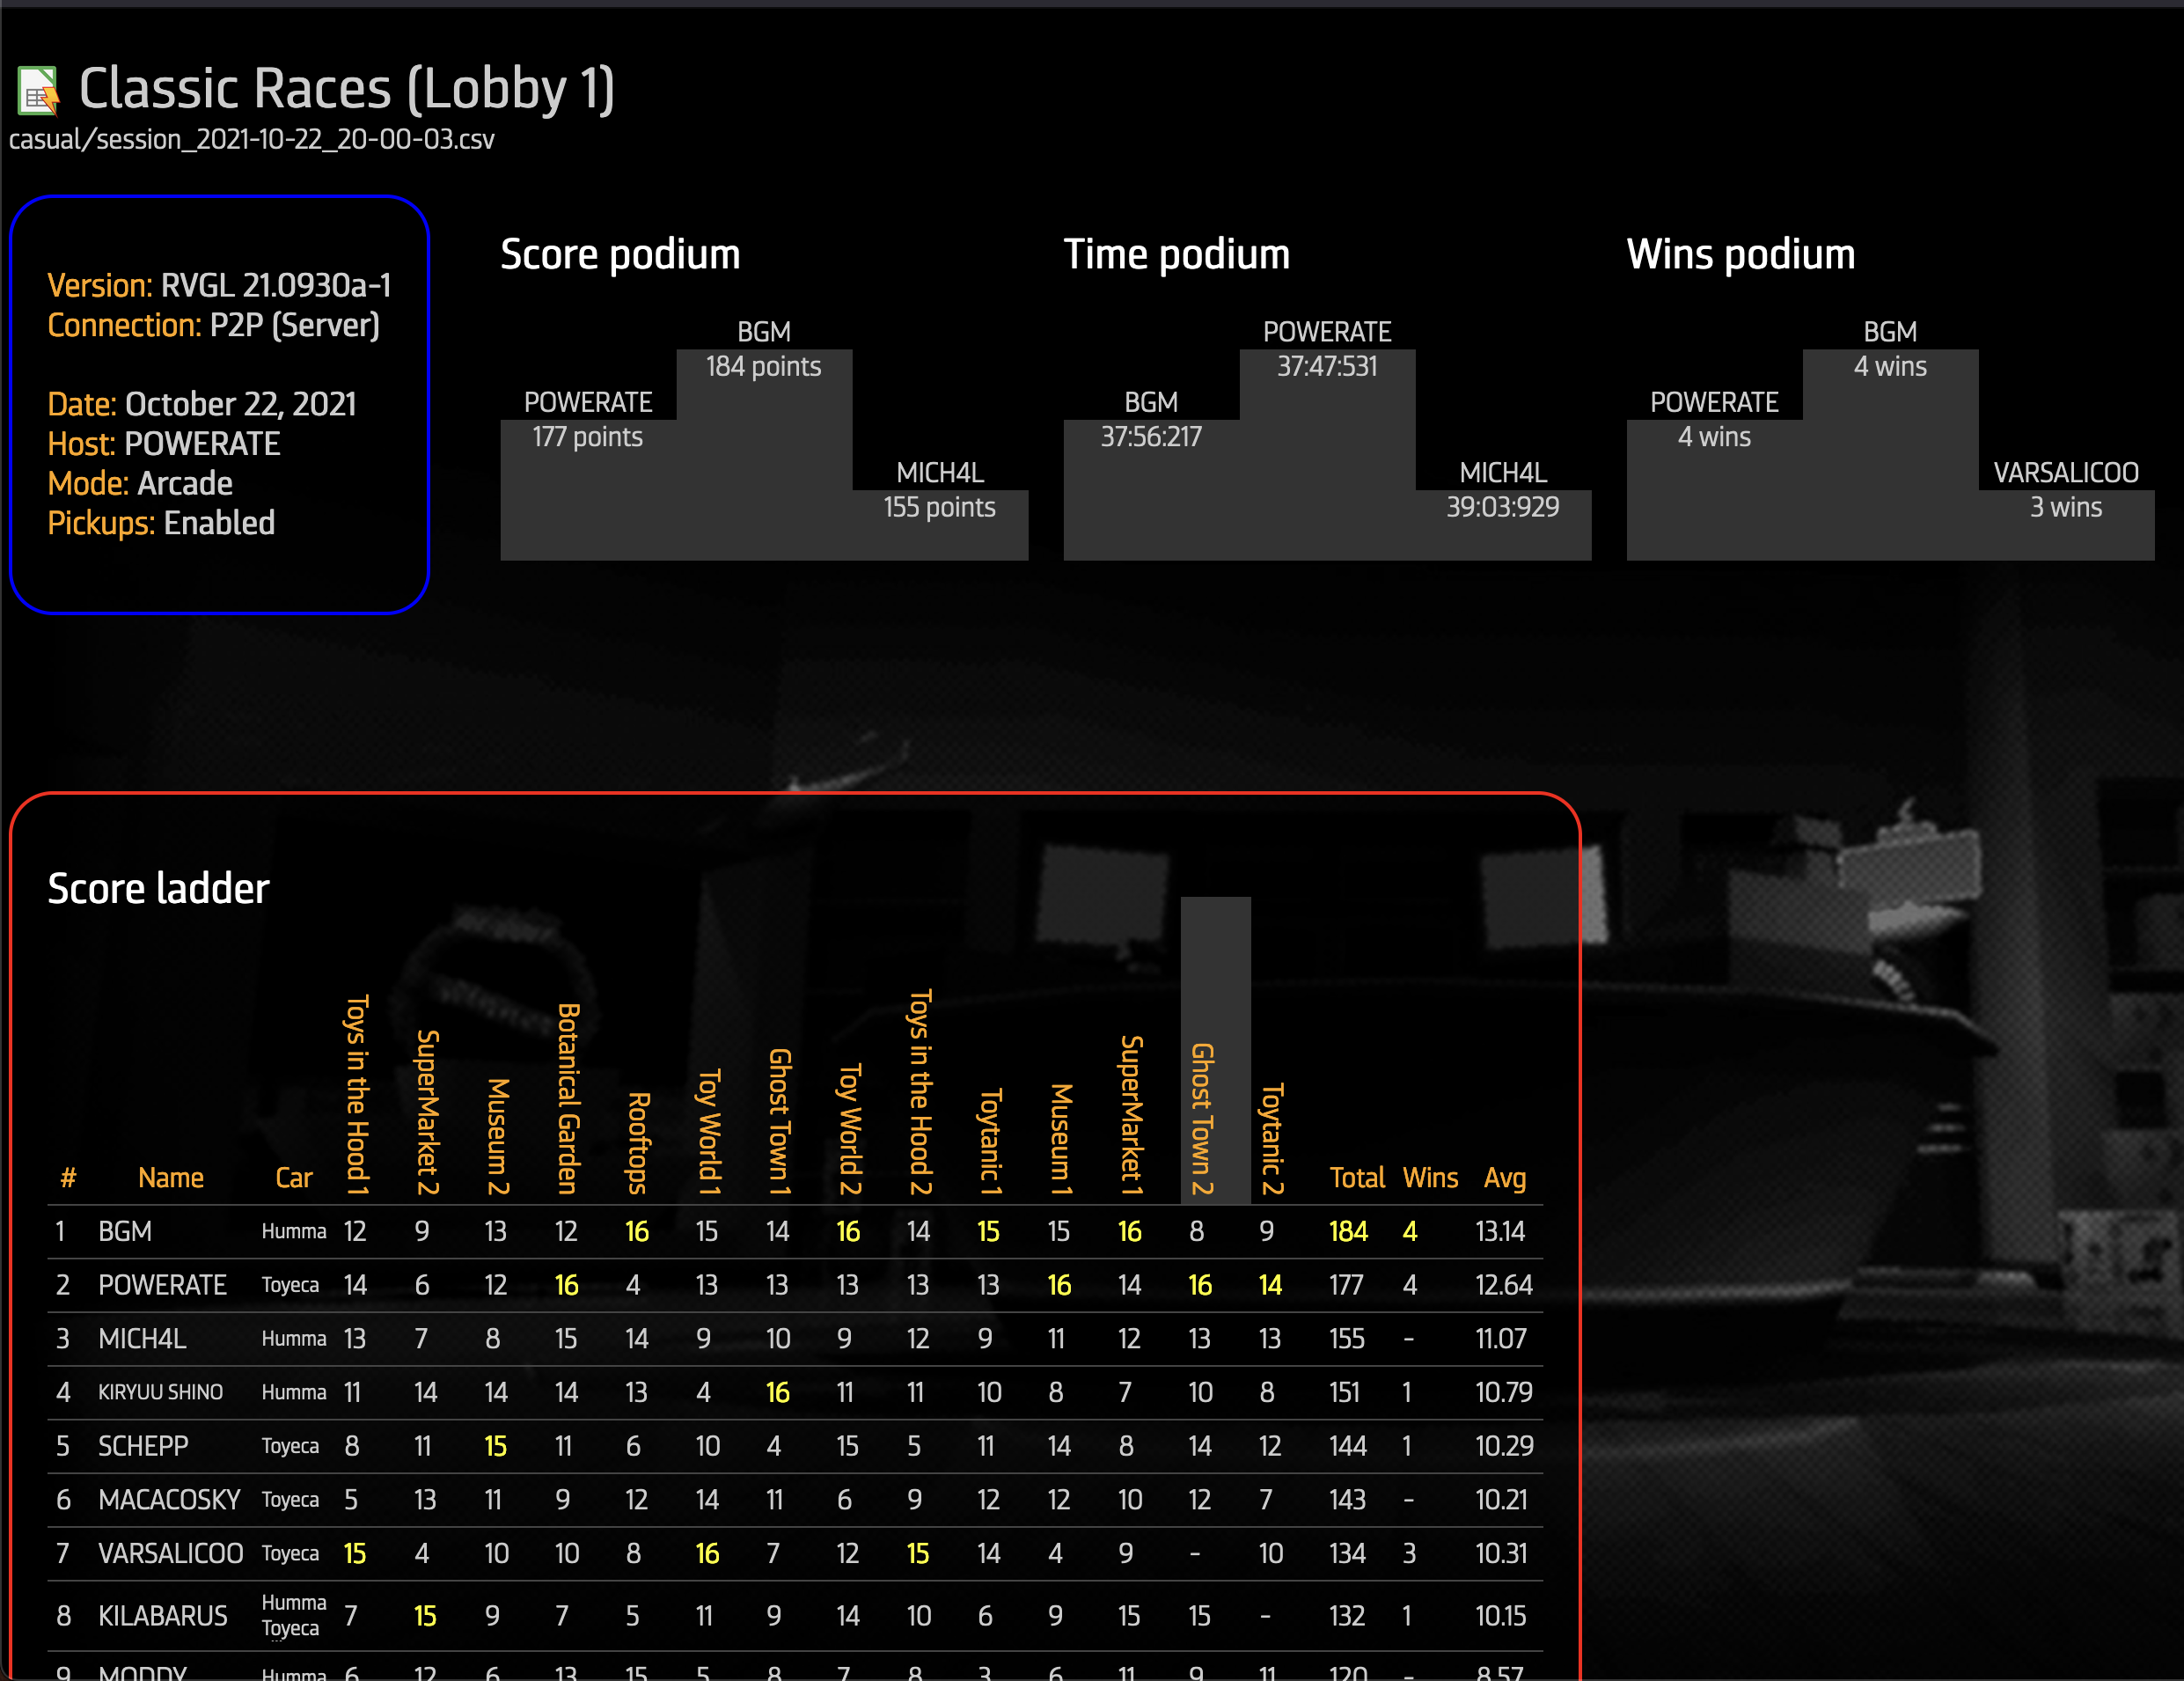
\includegraphics[width=17cm, height=15cm]{img/io-results.png}

\section{Justificación del Problema}
Actualmente, no existe ninguna plataforma que permita a los usuarios registrarse o visualizar resultados y estadísticas de las sesiones multijugador organizadas por la comunidad. Lo anterior significa que, cuando se juegan partidas online, no es posible obtener de manera automática rankings, estadísticas por vehículo y menos por usuario, ya que no hay forma de vincular, de manera definitiva, a los jugadores a través de un perfil dentro del juego. Es por ello que un usuario de nuestra comunidad, actualmente, no puede saber cuántas carreras o sesiones ha ganado con cierto auto, o en cierta pista, cómo se compara al resto, qué porcentaje de carreras ha perdido, etc.





% Proyecto
\chapter{Proyecto}

\section{Objetivo General del Proyecto}
Desarrollar una aplicación web para Re-Volt America, la comunidad del continente americano formada alrededor del videojuego de carreras Re-Volt, 1999. Esta aplicación permite centralizar toda la actividad multijugador en el juego de dicha comunidad, dejando a los usuarios crear cuentas en la web con un perfil asociado. En dicho perfil se podrán visualizar resultados oficiales de las sesiones de carreras que se organicen, además de estadísticas personales.

\section{Objetivos Específicos del Proyecto}
1.	Elaborar una propuesta que consiga atender las necesidades y problemas de los usuarios de Re-Volt America en relación con el almacenamiento y visualización de resultados de partidas online, además de proveer visibilidad a la comunidad en general.
2.	Diseñar la solución de software de procesamiento de datos de sesiones multijugador de Re-Volt, creando interfaces que les permitan a los jugadores visualizar resultados oficiales de las sesiones de carreras en línea, además de estadísticas personales. De esta forma, el diseño de la aplicación en su conjunto centralizará toda la actividad de la comunidad en una sola web.
3.	Implementar la aplicación web, la cual permitirá a los organizadores de sesiones de carreras en línea subir y publicar los resultados de dichas carreras, además de realizar el lazo entre jugadores y cuentas de usuario de esta. El software implementado permitirá a su vez procesar dicha información subida a la web, y así poder mostrar a los usuarios finales una vista clara de sus resultados en carreras y las estadísticas personales.

\section{Metodología de Desarrollo}
Luego de analizar a fondo el proyecto, se concluyó que en lo que respecta al problema se cuenta con una experiencia en el área y complejidad altas, pero con un tamaño pequeño, lo cual representa un bajo riesgo en lo que respecta al problema. Por otra parte, en relación con el software se cuenta con una alta experiencia en términos técnicos. Además, el software en si tiene una complejidad y tamaño pequeños, por lo que el riesgo es realmente bajo en lo que a este respecta. En conclusión, el riesgo ponderado entre el problema y el software a desarrollar es muy bajo.
Según la evaluación del proyecto, se concluyó que este tiene un riesgo total asociado muy bajo, por lo que se contaría con la libertad de utilizar cualquier tipo de metodología de desarrollo para llevarlo a cabo. Como contamos con esta libertad de elección, se buscará sacar provecho de ella, y se ha seleccionado una metodología de desarrollo iterativa, a través de la cual se desarrollará en ciclos. Estos ciclos permitirán al software evolucionar a medida que se recibe retroalimentación por parte de los usuarios, corrigiendo errores y mejorando detalles a medida que se progresa en el desarrollo de la aplicación. Según el contexto en el que se desarrollará esta aplicación, los usuarios de la comunidad tendrán una importante incidencia en el testeo y uso diario de la misma, lo cual implica que estarán presentes durante el proceso de implementación de varias de las funcionalidades que se pretenden lograr con esta propuesta. Se sabe también con antelación que los usuarios estarán dispuestos a ayudar con las pruebas y el testeo de la aplicación. Esta opción fue seleccionada ya que:

\begin{enumerate}
	\item Permite más flexibilidad en cuanto a lo que se planea desarrollar como aplicación web, debido a que a medida que avance el proyecto es muy probable que surjan cambios o nuevas ideas a partir de la retroalimentación recibida de la comunidad.
	\item Debido a la naturaleza del proyecto, utilizar una metodología iterativa es muy beneficioso ya que ésta permitirá una constante supervisión de los cambios realizados al software, lo que finalmente se traducirá en menos errores, y un producto final que se ajuste y esté a la altura de las necesidades de la comunidad.
	\item Con una metodología iterativa será posible contar con prototipos que la comunidad pueda comenzar a utilizar, y a su vez adaptarse a las interfaces y funcionalidades de la aplicación mientras esta se encuentra en desarrollo. Esto es muy importante ya que las sesiones multijugador suelen organizarse a diario, por lo que mientras antes se cuente con una solución funcional, antes podrá la comunidad comenzar a llevar un registro histórico de las partidas online que organiza.
\end{enumerate}

\section{Técnicas y Notaciones}
ejemplo: Diagramas de Casos de Uso -notación UML es utilizada para detallar la funcionalidad del software

\section{Estándares de Documentación}
Agregar estándares...

\section{Herramientas, Frameworks y  Lenguajes Utilizados}
\begin{itemize}
	\item Ruby versión 3.2.2: Lenguaje de programación de alto nivel.
	\item HAML: Lenguaje de marcado para la abstracción de HTML.
	\item Ruby on Rails versión 7: Framework para desarrollo de aplicaciones web fullstack.
	\item MongoDB versión 3: Base de datos orientada a documentos JSON.
	\item MongoDBCompass versión 1.39.0: Visor para la base de datos en MongoDB.
	\item Redis versión 7: Programa de almacenamiento en memoria, utilizado para el caché de datos.
	\item RedisInsight versión 2.30.0: Visor para el almacenamiento del caché en Redis.
	\item NodeJS versión 16: Entorno de servidor multiplataforma utilizado para la conversión de archivos en runtime.
	\item Yarn versión 1.22: Gestor de paquetes para JavaScript.
	\item Docker versión 24.0.2: Tecnología que permite crear y utilizar contenedores de Linux. Para efectos de este proyecto fue utilizado con el fin de probar el software desarrollado en la distribución de Linux requerida.
\end{itemize}







% Factibilidad
\chapter{Factibilidad}

\section{Factibilidad Técnica}
\subsection{Conocimientos de los Usuarios}
Para el correcto funcionamiento de la aplicación propuesta, es de esperar que los distintos miembros del staff de RVA, quienes serán los principales usuarios del software, deban tener determinados conocimientos para poder operarla con éxito.

Gracias a que, naturalmente, el staff de RVA lleva un largo tiempo manejando la comunidad y los resultados de las sesiones organizadas, no hace falta mayor capacitación técnica en cuanto al funcionamiento del cálculo de puntos, multiplicadores de autos, y demás características específicas del sistema de RVA. Para efectos de factibilidad técnica, el staff ya cuenta con los conocimientos necesarios para poder migrar a un sistema que sólo busca mejorar y facilitar los procesos actuales.

En cuanto a la aplicación propuesta en este proyecto y su funcionamiento operacional, el staff será habituado al nuevo sistema mediante un video de inducción a la nueva plataforma web. También se asignará un periodo de prueba para que puedan utilizar la página ellos mismos, y así puedan adaptarse fácilmente.

\subsection{Disponibilidad Profesional}
Para el desarrollo de la aplicación propuesta, se necesita del trabajo de un profesional en el área del desarrollo de software, el cual sea capaz de satisfacer las necesidades de RVA y cumplir los objetivos de desarrollo propuestos.

Para efectos de este proyecto, se cuenta tanto con el tiempo profesional, como también con los conocimientos técnicos requeridos.

Adicionalmente, se cuenta con el equipo físico para poder desarrollar la aplicación, como puede ser un computador, acceso a internet y demás software para desarrollo. A continuación, se presentan tablas de especificación de los equipos físicos y el software con el que se cuenta para desarrollar la aplicación.

% Equipos Físicos
\begin{center}
	\begin{tabular}{ | l | p{10cm} |}
		\hline
		\multicolumn{2}{|c|}{\textbf{Equipos Físicos}} \\
		\hline
		\multicolumn{1}{|c|}{\textbf{Nombre}} & \multicolumn{1}{|c|}{\textbf{Acceso}} \\
		\hline
		{\textbf{Windows PC}} & Equipo personal \\ \hline
		
		{\textbf{MacBook Pro M1}} & Equipo personal \\ \hline
	\end{tabular}
\end{center}

% Software
\begin{center}
	\begin{tabular}{ | l | p{10cm} |}
		\hline
		\multicolumn{2}{|c|}{\textbf{Software}} \\
		\hline
		\multicolumn{1}{|c|}{\textbf{Nombre}} & \multicolumn{1}{|c|}{\textbf{Acceso}} \\
		\hline
		
		{\textbf{Notepad++}} & Software libre \\ \hline
		
		{\textbf{MongoDB Compass}} & Software libre \\ \hline
		
		{\textbf{RedisInsight}} & Software libre \\ \hline
		
		{\textbf{Git/Git Bash}} & Software libre \\ \hline
		
		{\textbf{Ubuntu LTS}} & Software libre \\ \hline
		
		{\textbf{RubyMine}} & Licencia de estudiante \\ \hline
		
		{\textbf{Termius}} & Licencia de estudiante \\ \hline
		
		{\textbf{Microsoft Excel}} & Licencia de estudiante \\ \hline
	\end{tabular}
\end{center}

\subsection{Despliegue y Servidor}
Para realizar el despliegue de la aplicación a desarrollar, se ha escogido un servidor de tipo VPS (Servidor Virtual Privado). Las especificaciones técnicas de dicho servidor son las siguientes:

% Servidor
\begin{center}
	\begin{tabular}{ | l | p{10cm} |}
		\hline
		\multicolumn{2}{|c|}{\textbf{VPS}} \\
		\hline
		\multicolumn{1}{|c|}{\textbf{Característica}} & \multicolumn{1}{|c|}{\textbf{Detalle}} \\
		\hline
		
		{\textbf{Proveedor}} & DigitalOcean \\ \hline
		
		{\textbf{Región}} & Nueva York \\ \hline
		
		{\textbf{Sistema Operativo}} & Ubuntu 22.04 (LTS) x64 \\ \hline
		
		{\textbf{Tipo de CPU}} & Intel Regular \\ \hline
		
		{\textbf{Número de vCPUs}} & 1 CPU\\ \hline
		
		{\textbf{Memoria}} & 2 GB \\ \hline
		
		{\textbf{Almacenamiento (SSD)}} & 50 GB \\ \hline
		
		{\textbf{Transferencia}} & 2 TB \\ \hline
	\end{tabular}
\end{center}

El software instalado en este servidor para el despliegue de la aplicación es el mismo especificado en la \autoref{project:software}.

\section{Factibilidad Operativa}
En cuanto a la factibilidad operativa de este proyecto, se sabe que el staff de Re-Volt America tiene gran disposición al cambio, ya que el sistema antiguo no solamente les demanda demasiado tiempo y esfuerzo, sino que, además, resulta poco preciso y muy propenso a errores en su uso diario debido a la gran cantidad de pasos manuales que este conlleva.

La factibilidad operativa es fácilmente demostrada al comparar la solución propuesta con el sistema que esta pretende reemplazar. Vale decir que, actualmente, quienes hacen uso del sistema de hojas de cálculo maestras en Excel y la aplicación de RVA-Points para el procesamiento de las sesiones, verían su trabajo facilitado en todos los sentidos al contar con una plataforma que se encargue de llevar la cuenta de todo, procesar los resultados y mantener los rankings y temporadas al día de manera automática y confiable.

\section{Factibilidad Económica}
A continuación se presenta un detalle de tablas de costos y el flujo de caja asociado al proyecto. 

\subsection{Tablas de Costos}
\label{feasibility:costs}
En esta sección se presentan dos tablas de costos relacionadas al proyecto. La primera tabla contiene todo el software utilizado para el desarrollo de este proyecto, mientras que la segunda tabla contempla los costos inherentes de RVA, combinando aquellos costos adquiridos que vienen de antes del despliegue a producción del software que se ha desarrollado.

% Equipos Físicos
\begin{center}
	\begin{tabular}{ | l | p{5cm} | p{5cm}|}
		\hline
		\multicolumn{3}{|c|}{\textbf{Software}} \\
		\hline
		\multicolumn{1}{|c|}{\textbf{Nombre}} & \multicolumn{1}{|c|}{\textbf{Acceso}} & \multicolumn{1}{|c|}{\textbf{Precio (anual)}} \\
		\hline
		{\textbf{Notepad++}} & Software libre & \multicolumn{1}{|r|}{\$0} \\ \hline

		{\textbf{MongoDB Compass}} & Software libre & \multicolumn{1}{|r|}{\$0} \\ \hline
		
		{\textbf{RedisInsight}} & Software libre & \multicolumn{1}{|r|}{\$0} \\ \hline
		
		{\textbf{Git/Git Bash}} & Software libre & \multicolumn{1}{|r|}{\$0} \\ \hline
		
		{\textbf{Ubuntu LTS}} & Software libre & \multicolumn{1}{|r|}{\$0} \\ \hline
		
		{\textbf{RubyMine}} & Licencia de estudiante & \multicolumn{1}{|r|}{\$0} \\ \hline
		
		{\textbf{Termius}} & Licencia de estudiante & \multicolumn{1}{|r|}{\$0} \\ \hline
		
		{\textbf{Microsoft Excel}} & Licencia de estudiante & \multicolumn{1}{|r|}{\$0} \\ \hline
	\end{tabular}
\end{center}

% Costos de Producción
\begin{center}
	\begin{tabular}{ | l | p{5cm} | p{5cm}|}
		\hline
		\multicolumn{3}{|c|}{\textbf{Costos de Producción}} \\
		\hline
		\multicolumn{1}{|c|}{\textbf{Nombre}} & \multicolumn{1}{|c|}{\textbf{Proveedor}} & \multicolumn{1}{|c|}{\textbf{Precio (anual)}} \\
		\hline
		{\textbf{VPS}} & DigitalOcean & \multicolumn{1}{|r|}{\$125.000} \\ \hline
		
		{\textbf{Mailer}} & Postmark & \multicolumn{1}{|r|}{\$156.000} \\ \hline
		
		{\textbf{Dominio (rva.lat)}} & Namecheap & \multicolumn{1}{|r|}{\$22.600} \\ \hline
		
		{\textbf{Git/Git Bash}} & Software libre & \multicolumn{1}{|r|}{\$0} \\ \hline
		
		{\textbf{Ubuntu LTS}} & Software libre & \multicolumn{1}{|r|}{\$0} \\ \hline
		
		{\textbf{RubyMine}} & Licencia de estudiante & \multicolumn{1}{|r|}{\$0} \\ \hline
		
		{\textbf{Termius}} & Licencia de estudiante & \multicolumn{1}{|r|}{\$0} \\ \hline
		
		{\textbf{Microsoft Excel}} & Licencia de estudiante & \multicolumn{1}{|r|}{\$0} \\ \hline
	\end{tabular}
\end{center}

Cabe destacar que, dentro de los costos de producción, tanto el precio anual del VPS como el del dominio de RVA son costos adquiridos que han sido mantenidos desde antes de la puesta en marcha de este proyecto. Su mención en la tabla anterior es puramente una formalidad.

\subsection{Flujo de Caja}
Para la redacción del flujo de caja y la confección de sus tablas asociadas, se debe tener en cuenta que existen contextos económicos internos diferentes dentro de la evolución de RVA como proyecto.

En segundo lugar, se hablará de una proyección de lo que costará, en términos económicos, mantener el software desarrollado para este proyecto a futuro desde su finalización.

La valorización del tiempo de trabajo será determinada, en ambos casos, a partir de promedios y estimaciones que pueden encontrarse hoy en día en el mercado del desarrollo de software. Las referencias serán mencionadas oportunamente.

\subsubsection{Contexto e Indicadores Económicos}
\label{feasibility:economic:context}
La Tasa Mínima Aceptable de Rendimiento (TMAR) para proyectos de desarrollo de software, a la cual llamaremos ''\textit{r}'', ha sido calculada para este proyecto a partir de la inflación promedio anual reportada por el Banco Central de Chile, y la prima de riesgo asociada a proyectos tecnológicos reportada por el Standish Group International en 2011 (CHAOS Manifesto).

% Tasa Anual
\begin{center}
	\begin{tabular}{ | p{7cm} | p{5cm}|}
		\hline
		{\textbf{Inflación Promedio Anual}} & 4.3\%  \\ \hline
		{\textbf{Tasa Prima de Riesgo}} & 21\% \\ \hline
	\end{tabular}
\end{center}

Con la inflación promedio anual y la tasa prima de riesgo, es posible calcular el valor de la TMAR asociada al proyecto.

\[
\mathlarger{
  r = 0.04+0.21+(0.04\cdot0.21) = 0.2584 \approx 26\%
}
\]

\subsubsection{Puesta en Marcha}
\label{feasibility:economic:startup}
A partir de los datos obtenidos en la \autoref{feasibility:economic:context}, es posible realizar un cálculo del valor actual neto (VAN) del proyecto. En este caso, todos los costos asociados figurarán como un ahorro para la comunidad de RVA, ya que debemos considerar que todo lo realizado vendría representar dinero que, potencialmente, la comunidad hubiese tenido que gastar en otro profesional y recursos de no haberse desarrollado el software en cuestión.

La valorización del tiempo empleado en el desarrollo de software a lo largo del proyecto está basada en el sueldo promedio de un analista programador en Chile según Talent.com (\$900.000 mensual; \$5.538 por hora), ajustado a las horas de trabajo efectivas empleadas en el proyecto, las cuales fueron 4 horas de trabajo efectivo durante 6 días de la semana por mes (4 semanas) de desarrollo.

\[
\mathlarger{
	Desarrollo = \$5.538 \cdot \left(4 \textit{ horas}\cdot6 \textit{ días}\cdot4 \textit{ semanas}\right) = \$531.648
}
\]

Además del tiempo valorizado, también se ha estimado una valorización de los costos de internet y electricidad asociados con el proyecto, basados en su costo promedio mensual y dividiéndolos por la mitad, para así obtener un valor realista.

\[
	Internet = \frac{\$20.000}{2} = \$10.000
\]

\[
	Electricidad = \frac{\$40.000}{2} = \$20.000
\]

A continuación, se presenta una tabla que contiene los gastos mensuales estimados asociados a la puesta en marcha del proyecto:

% Costos Mensuales
\begin{center}
	\begin{tabular}{ | p{5cm} | p{5cm} | }
		\hline
    \multicolumn{2}{|c|}{\textbf{Costos}} \\
		\hline
		{\textbf{Desarrollo}} & \multicolumn{1}{|r|}{\$531.648} \\ \hline
		
		{\textbf{Internet}} & \multicolumn{1}{|r|}{\$10.000} \\ \hline
		
		{\textbf{Electricidad}} & \multicolumn{1}{|r|}{\$20.600} \\ \hline
    
    {\textbf{Total}} & \multicolumn{1}{|r|}{\$561.648} \\ \hline
	\end{tabular}
\end{center}

Una vez calculado el total de gastos para la puesta en marcha, es posible extrapolar a 4 meses y calcular la inversión inicial del proyecto a través de la siguiente fórmula.

\[
\mathlarger{
	{I_0} = \$561.648 \cdot 4\textit{ meses}= \$2.246.592
}
\]

\subsubsection{Cálculo del Valor Actual Neto}
Siguiendo con la lógica de la valorización de las horas de trabajo efectivas, se tiene que, una vez terminado el proyecto (al final de los 4 meses), la cantidad de horas efectivas necesarias para mantener el proyecto a lo largo del tiempo disminuirá sustancialmente.

Se dirá que, si antes eran 4 las horas efectivas en 6 días de la semana, ahora sólo será 1 hora por 5 días de la semana, ya que el trabajo requerido por la comunidad ya no será de desarrollo de software, sino que de mantención, realización de mejoras oportunas, y soporte para la plataforma.

\[
\mathlarger{
	Mantenimiento = \$5.538 \cdot \left(1 \textit{ horas}\cdot5 \textit{ días}\cdot4 \textit{ semanas}\right) = \$110.760
}
\]

Además de lo anterior, se realiza un ajuste proporcional del costo de internet y electricidad en función de las valorizaciones del tiempo de desarrollo y mantenimiento calculadas.

\[
\frac{Desarrollo}{Mantenimiento} = \frac{\$531.648}{\$110.760} = 4.8
\]

\[
Internet = \frac{\$10.000}{4.8} = \$2.083
\]

\[
Electricidad = \frac{\$20.600}{4.8} = \$5.208
\]

Si proyectamos a 5 años, podemos calcular el Valor Actual Neto (VAN) de ahorro para el proyecto.

% VAC Mantenimiento
\begin{center}
	\begin{tabular}{ | l | l | l | l | l | l | l |}
		\hline
		& \multicolumn{1}{|c|}{\textbf{0}} & \multicolumn{1}{|c|}{\textbf{1}} & \multicolumn{1}{|c|}{\textbf{2}} & \multicolumn{1}{|c|}{\textbf{3}} & \multicolumn{1}{|c|}{\textbf{4}} & \multicolumn{1}{|c|}{\textbf{5}} \\
		\hline
		{\textbf{Mantenimiento}} &  & \multicolumn{1}{|r|}{\$1.329.120} & \multicolumn{1}{|r|}{\$1.329.120} & \multicolumn{1}{|r|}{\$1.329.120} & \multicolumn{1}{|r|}{\$1.329.120} & \multicolumn{1}{|r|}{\$1.329.120} \\ \hline
		
		{\textbf{Internet}} &  & \multicolumn{1}{|r|}{\$24.996} & \multicolumn{1}{|r|}{\$24.996} & \multicolumn{1}{|r|}{\$24.996} & \multicolumn{1}{|r|}{\$24.996} & \multicolumn{1}{|r|}{\$24.996} \\ \hline
		
		{\textbf{Electricidad}} &  & \multicolumn{1}{|r|}{\$62.496} & \multicolumn{1}{|r|}{\$62.496} & \multicolumn{1}{|r|}{\$62.496} & \multicolumn{1}{|r|}{\$62.496} & \multicolumn{1}{|r|}{\$62.496} \\ \hline
		
		{\textbf{Hosting}} &  & \multicolumn{1}{|r|}{-\$126.312} & \multicolumn{1}{|r|}{-\$126.312} & \multicolumn{1}{|r|}{-\$126.312} & \multicolumn{1}{|r|}{-\$126.312} & \multicolumn{1}{|r|}{-\$126.312} \\ \hline
		
		{\textbf{Flujo}} &  & \multicolumn{1}{|r|}{\$1.290.300} & \multicolumn{1}{|r|}{\$1.290.300} & \multicolumn{1}{|r|}{\$1.290.300} & \multicolumn{1}{|r|}{\$1.290.300} & \multicolumn{1}{|r|}{\$1.290.300} \\ \hline
		{\textbf{Inv. Inicial}} & \multicolumn{1}{|r|}{\$2.246.592} & & & & & \\ \hline
		\textbf{Flujo Total} & \multicolumn{1}{|r|}{\$6.451.500} & & & & & \\ \hline
	\end{tabular}
\end{center}

Como clarificación general para la siguiente fórmula, el número de años de proyección vendrá definido como ''\textit{n}'', y ''\textit{C}'' representará los flujos de caja.

Asimismo, recordar también que ''\textit{r}'' representa la TMAR del proyecto calculada en la \autoref{feasibility:economic:context}, e ''\textit{I\textsubscript{0}}'' representa la inversión inicial calculada en la \autoref{feasibility:economic:startup}.

\[
\mathlarger{
	{VAN} = I_0 + \sum\limits_{t=i}^{n}\frac{C_t}{\left(1+r^t\right)} = \$5.646.624
}
\]

https://www.bcentral.cl/web/banco-central/contenido/-/detalle/informe-de-politica-monetaria-septiembre-2023 (INFLACIÓN)

https://www.immagic.com/eLibrary/ARCHIVES/GENERAL/GENREF/ChaosManifest\_2011.pdf (TASA DE RIESGO)

https://radio.uchile.cl/2023/04/13/cuentas-de-electricidad-de-hogares-de-mayor-consumo-subiran-entre-10-y-16/

https://www.ine.gob.cl/estadisticas/economia/transporte-y-comunicaciones/estructura-del-transporte-por-carretera/2020/05/16/conexiones-a-internet-en-hogares-del-pa%C3%ADs-aumentaron-en-m%C3%A1s-de-670.000-en-los-%C3%BAltimos-cinco-a%C3%B1os

https://cl.talent.com/salary?job=analista+programador

\section{Conclusión de Factibilidad}
Para concluir, podemos decir que en cuanto a los distintos tipos de factibilidad evaluados se cuenta con usuarios técnicamente capaces y con la disponibilidad profesional necesaria para el desarrollo del proyecto. Por el lado operativo, existe disposición al cambio por parte de los administradores y el staff en general. Económicamente, a partir de los costos y beneficios recopilados, se ha obtenido que existe un valor económico sustancial asociado al proyecto.

Gracias al análisis realizado en los puntos anteriores, se puede concluir que el proyecto es factible.


% Arquitectura de Re-Volt America

% Requerimientos del Software
\chapter{Requerimientos del Software}

\section{Límites}
La aplicación no permitirá relacionar automáticamente cualquier nombre de jugador con su perfil dentro de la misma. Esto quiere decir que la aplicación estará limitada a relacionar el nombre que sea subido mediante el Session Log con un perfil que exista previamente en la plataforma.
La aplicación no permitirá el uso de su API de por parte de terceros, lo que quiere decir que la API de RVA estará limitada a la misma aplicación.

\section{Objetivo General del Software}
El sistema manejará información del proceso de cálculo de resultados de carreras para que la comunidad centralice los rankings y estadísticas por usuario dentro del mismo, es decir, reducirá el trabajo manual requerido actualmente para este procesamiento de resultados, y así hará más eficiente todo el proceso que conlleva mantener los rankings actualizados.


\subsection{Objetivos Específicos del Software}
•	El sistema permite que los administradores de la comunidad puedan subir los archivos de resultados generados por RVGL y, de esta forma, los resultados son generados automáticamente dentro de la aplicación. Esto elimina el tiempo de los organizadores de calcular los resultados manualmente.

•	El sistema permite que los usuarios puedan ver sus estadísticas en tiempo real, lo que elimina la necesidad de llevar la cuenta de manera manual por cada uno de ellos.

•	El sistema permite enlazar los nombres de usuario utilizados en las sesiones multijugador de RVGL a perfiles dentro de la aplicación, lo cual hace posible la recopilación y atribución de métricas individuales por jugador, y agiliza la visualización de resultados.

•	El sistema permite llevar un registro histórico de manera automática según se suben y se procesan los archivos de resultados en la aplicación, lo cual elimina completamente la necesidad de la comunidad de mantener toda esta información actualizada de manera manual.


\section{Requerimientos Funcionales del Software}

% Autos
\begin{center}
	\begin{tabular}{ | l | p{15cm} |}
		\hline
		\multicolumn{2}{|c|}{\textbf{Módulo de Registros de Autos de Re-Volt America}} \\
		\hline
		\multicolumn{1}{|c|}{\textbf{Id}} & \multicolumn{1}{|c|}{\textbf{Descripción}} \\
		\hline
		RF\_01 & La plataforma contará con un módulo de creación de autos. Los autos deben contar con todos los parámetros obligatorios. Sólo los administradores pueden crear autos. \\ \hline

		RF\_02 & La plataforma contará con un módulo de visualización de autos. El listado estará separado por temporadas y por clases de autos. Este módulo estará disponible para cualquier tipo de usuario. \\ \hline

		RF\_03 & La plataforma contará con un módulo de edición de un auto, los cuales deben contar con todos los parámetros obligatorios para ser modificados. Este módulo estará disponible sólo para los administradores. \\ \hline
		
		RF\_04 & La plataforma contará con un módulo de eliminación de un auto. La eliminación no tendrá efectos secundarios a nivel de la base de datos, ya que la aplicación estará preparada para manejar excepciones cuando las entradas de corredores estén asociadas a un auto que no exista. Este módulo sólo estará disponible para administradores. \\ \hline
		
		RF\_05 & La plataforma contará con un módulo de visualización de un solo auto. En esta vista se podrán ver todos los parámetros del auto. Este módulo estará disponible sólo para los administradores. \\ \hline
	\end{tabular}
\end{center}

% Pistas
\begin{center}
	\begin{tabular}{ | l | p{15cm} |}
		\hline
		\multicolumn{2}{|c|}{\textbf{Módulo de Registros de Pistas de Re-Volt America}} \\
		\hline
		\multicolumn{1}{|c|}{\textbf{Id}} & \multicolumn{1}{|c|}{\textbf{Descripción}} \\
		\hline
		RF\_06 & La plataforma contará con un módulo de creación de pistas. Las pistas deben contar con todos los parámetros obligatorios. Sólo los administradores pueden crear pistas. \\ \hline
		
		RF\_07 & La plataforma contará con un módulo de visualización de pistas. El listado estará separado por temporadas y por clases de pistas. Este módulo estará disponible para cualquier tipo de usuario. \\ \hline
		
		RF\_08 & La plataforma contará con un módulo de edición de una pista, las cuales deben contar con todos los parámetros obligatorios para ser modificadas. Este módulo estará disponible sólo para los administradores. \\ \hline
		
		RF\_09 & La plataforma contará con un módulo de eliminación de una pista. La eliminación no tendrá efectos secundarios a nivel de la base de datos, ya que la aplicación estará preparada para manejar excepciones cuando las carreras estén asociadas a una pista que no exista. Este módulo sólo estará disponible para administradores. \\ \hline
		
		RF\_10 & La plataforma contará con un módulo de visualización de un solo pista. En esta vista se podrán ver todos los parámetros de la pista. Este módulo estará disponible sólo para los administradores. \\ \hline
	\end{tabular}
\end{center}

% Temporadas
\begin{center}
	\begin{tabular}{ | l | p{15cm} |}
		\hline
		\multicolumn{2}{|c|}{\textbf{Módulo de Registros de Temporadas de Re-Volt America}} \\
		\hline
		\multicolumn{1}{|c|}{\textbf{Id}} & \multicolumn{1}{|c|}{\textbf{Descripción}} \\
		\hline
		RF\_11 & La plataforma contará con un módulo de creación de temporadas. Las temporadas deben contar con todos los parámetros obligatorios. Sólo los administradores pueden crear temporadas. \\ \hline
		
		RF\_12 & La plataforma contará con un módulo de visualización de temporadas. El listado contendrá todos los rankings asociados a esta temporada. Este módulo estará disponible para cualquier tipo de usuario. \\ \hline
		
		RF\_13 & La plataforma contará con un módulo de edición de una temporada, las cuales deben contar con todos los parámetros obligatorios para ser modificados. Este módulo estará disponible sólo para los administradores. \\ \hline
		
		RF\_14 & La plataforma contará con un módulo de eliminación de una temporada. La eliminación no tendrá efectos secundarios a nivel de la base de datos, ya que la aplicación estará preparada para manejar excepciones cuando los rankings estén asociados a una temporada que no existe. Este módulo sólo estará disponible para administradores. \\ \hline
		
		RF\_15 & La plataforma contará con un módulo de visualización de una sola temporada. En esta vista se podrán ver todos los parámetros de la temporada. Este módulo estará disponible sólo para los administradores. \\ \hline
	\end{tabular}
\end{center}

% Rankings
\begin{center}
	\begin{tabular}{ | l | p{15cm} |}
		\hline
		\multicolumn{2}{|c|}{\textbf{Módulo de Registros de Rankings de Re-Volt America}} \\
		\hline
		\multicolumn{1}{|c|}{\textbf{Id}} & \multicolumn{1}{|c|}{\textbf{Descripción}} \\
		\hline
		RF\_16 & La plataforma contará con un módulo de creación de rankings. Los rankings deben contar con todos los parámetros obligatorios. Sólo los administradores pueden crear rankings. \\ \hline
		
		RF\_17 & La plataforma contará con un módulo de visualización de rankings. El listado estará separado por temporadas y por clases de rankings. Este módulo estará disponible para cualquier tipo de usuario. \\ \hline
		
		RF\_18 & La plataforma contará con un módulo de edición de un ranking, los cuales deben contar con todos los parámetros obligatorios para ser modificados. Este módulo estará disponible sólo para los administradores. \\ \hline
		
		RF\_19 & La plataforma contará con un módulo de eliminación de un ranking. La eliminación no tendrá efectos secundarios a nivel de la base de datos, ya que la aplicación estará preparada para manejar excepciones cuando las temporadas están asociadas a un ranking que no existe. Este módulo sólo estará disponible para administradores. \\ \hline
		
		RF\_20 & La plataforma contará con un módulo de visualización de un solo ranking. En esta vista se podrán ver todos los parámetros del ranking. Este módulo estará disponible sólo para los administradores. \\ \hline
	\end{tabular}
\end{center}


% Sesiones
\begin{center}
	\begin{tabular}{ | l | p{15cm} |}
		\hline
		\multicolumn{2}{|c|}{\textbf{Módulo de Subida de Sesiones de Re-Volt America}} \\
		\hline
		\multicolumn{1}{|c|}{\textbf{Id}} & \multicolumn{1}{|c|}{\textbf{Descripción}} \\
		\hline
		RF\_21 & La plataforma contará con un módulo de subida de sesiones en forma de archivo CSV. Sólo los administradores pueden subir sesiones. Este módulo deberá permitir al usuario seleccionar un archivo de tipo CSV. Las sesiones deben contar con todos los parámetros obligatorios. Sólo los administradores pueden crear sesiones. \\ \hline
		
		RF\_22 & La plataforma contará con un módulo de visualización de sesiones. El listado estará separado por temporadas y por clases de sesiones. Este módulo estará disponible para cualquier tipo de usuario. \\ \hline
		
		RF\_23 & La plataforma contará con un módulo de edición de una sesión, las cuales deben contar con todos los parámetros obligatorios para ser modificadas. Este módulo estará disponible sólo para los administradores. \\ \hline
		
		RF\_24 & La plataforma contará con un módulo de eliminación de una sesión. La eliminación no tendrá efectos secundarios a nivel de la base de datos. Este módulo sólo estará disponible para administradores. \\ \hline
		
		RF\_25 & La plataforma contará con un módulo de visualización de una sola sesión. En esta vista se podrán ver todos los parámetros de la sesión. Este módulo estará disponible sólo para los administradores. \\ \hline
	\end{tabular}
\end{center}

% Análisis Funcional
\chapter{Análisis Funcional}

\section{Actores}
\label{analysis:actors}
En el software desarrollado, cada rol dentro del staff de RVA ha sido considerado como un actor diferente. Para el contexto del presente proyecto, el cargo de cada actor corresponde a su nombre, lo que quiere decir que si un actor lleva por nombre ''Administrador'', se entenderá que su cargo es ''Administrador de la comunidad de RVA''. Sólo los jugadores no cuentan con un cargo dentro de RVA.

La especificación de todos los actores se puede encontrar a continuación en la tabla TABLENUM.

\begin{center}
	\begin{tabular}{| p{3cm} | p{4.5cm} | p{4.5cm} | p{2cm} |}
		\hline
		\multicolumn{4}{|c|}{\textbf{Actores}} \\
		\hline
		\multicolumn{1}{|c|}{\textbf{Actor}} & \multicolumn{1}{|c|}{\textbf{Función}} & \multicolumn{1}{|c|}{\textbf{Conocimientos}} & \multicolumn{1}{|c|}{\textbf{Privilegio}}\\
		\hline
		{\textbf{Administrador}} & Cumple con todas las funciones dentro de la comunidad como mantener autos, pistas, sesiones y manejo general del software. Configura el software para el resto de los usuarios. & Requiere conocimiento sobre como funciona el sistema en su totalidad, comprendiendo también el contexto en el que funciona RVA como comunidad. & Máximo. \\ \hline
		{\textbf{Organizador}} & Cumple con funciones específicamente relacionadas al manejo de sesiones multijugador y el procesamiento de los puntajes. & Requiere conocimiento específico de como subir archivos de sesión a la aplicación web, y un contexto general de como funciona RVA. & Intermedio (módulo de sesiones).\\ \hline
		{\textbf{Moderador}} & Utiliza las funciones específicas de manejo de usuarios, tal como la edición de perfiles o aplicación de infracciones. & Requiere conocimientos que se limitan al manejo de usuarios dentro de la web. & Intermedio (manejo de usuarios).\\ \hline
		{\textbf{Jugador}} & Utiliza la página sólo para visualizar la información que esta ofrece. & No requiere conocimientos técnicos más allá de iniciar sesión. & Ninguno.\\ \hline
	\end{tabular}
\end{center}

\newpage

\section{Casos de Uso}
Esta sección contiene todos los diagramas de casos de uso relevantes para el proyecto. Todos los casos de uso cuentan con su respectiva especificación y detalle según corresponda.

\subsection{Diagramas de Casos de Uso}
\label{analysis:usecases}

\begin{figure}[H]
  \begin{center}
    \includegraphics{privileges_module.png}
  \end{center}
  \caption[Diagrama de Casos de Uso del módulo de privilegios]{Diagrama de Casos de Uso del módulo de privilegios}
  \label{fig:privileges_module.png}
\end{figure}

\begin{figure}[H]
  \begin{center}
    \includegraphics{rva_cars_module_1.png}
  \end{center}
  \caption[Diagrama de Casos de Uso del módulo de autos 1]{Diagrama de Casos de Uso del módulo de autos 1}
  \label{fig:rva_cars_module_1}
\end{figure}

\begin{figure}[H]
  \begin{center}
    \includegraphics{rva_cars_module_2.png}
  \end{center}
  \caption[Diagrama de Casos de Uso del módulo de autos 2]{Diagrama de Casos de Uso del módulo de autos 2}
  \label{fig:rva_cars_module_2}
\end{figure}

\begin{figure}[H]
  \begin{center}
    \includegraphics{rva_tracks_module_1.png}
  \end{center}
  \caption[Diagrama de Casos de Uso del módulo de pistas 1]{Diagrama de Casos de Uso del módulo de pistas 1}
  \label{fig:rva_tracks_module_1}
\end{figure}

\begin{figure}[H]
  \begin{center}
    \includegraphics{rva_tracks_module_2.png}
  \end{center}
  \caption[Diagrama de Casos de Uso del módulo de pistas 2]{Diagrama de Casos de Uso del módulo de pistas 2}
  \label{fig:rva_tracks_module_2}
\end{figure}

\begin{figure}[H]
  \begin{center}
    \includegraphics{rva_seasons_module_1.png}
  \end{center}
  \caption[Diagrama de Casos de Uso del módulo de temporadas 1]{Diagrama de Casos de Uso del módulo de temporadas 1}
  \label{fig:rva_seasons_module_1}
\end{figure}

\begin{figure}[H]
  \begin{center}
    \includegraphics{rva_seasons_module_2.png}
  \end{center}
  \caption[Diagrama de Casos de Uso del módulo de temporadas 2]{Diagrama de Casos de Uso del módulo de temporadas 2}
  \label{fig:rva_seasons_module_2}
\end{figure}

\begin{figure}[H]
  \begin{center}
    \includegraphics{rva_sessions_module_1.png}
  \end{center}
  \caption[Diagrama de Casos de Uso del módulo de sesiones 1]{Diagrama de Casos de Uso del módulo de sesiones 1}
  \label{fig:rva_sessions_module_1}
\end{figure}

\begin{figure}[H]
  \begin{center}
    \includegraphics{rva_sessions_module_2.png}
  \end{center}
  \caption[Diagrama de Casos de Uso del módulo de sesiones 1]{Diagrama de Casos de Uso del módulo de sesiones 1}
  \label{fig:rva_sessions_module_2}
\end{figure}

\newpage

\subsection{Especificación de los Casos de Uso}
\label{analysis:usecases:specification}
En esta sección se detallan todos los casos de uso diagramados en la \autoref{analysis:usecases}. De acuerdo con la jerarquía de actores presentada en la \autoref{analysis:actors}, se entenderá que, si un actor de tipo ''Jugador'' puede realizar una acción específica, entonces cualquier otro de los actores con cargo podrá realizarla también.

A continuación, la tabla TABLENUM contiene los nombres y actores asociados a cada uno de los diagramas de casos de uso. Los casos de uso cuyos actores y nombre han sido marcados en negrita serán detallados posteriormente.

\begin{center}
  \begin{tabular}{| p{1.5cm} | p{6.5cm} | p{5.5cm} |}
    \hline
    \multicolumn{3}{|c|}{\textbf{Casos de Uso}} \\
    \hline
    \multicolumn{1}{|c|}{\textbf{Id}} & \multicolumn{1}{|c|}{\textbf{Actor}} & \multicolumn{1}{|c|}{\textbf{Nombre}}\\
    \hline
    
    % Módulo de Privilegios
    {\textbf{CU\_01}} & \textbf{Administrador, Moderador, Organizador y Jugador} & \textbf{Iniciar Sesión}\\ \hline
    
    % Módulo de Autos
    {\textbf{CU\_02}} & \textbf{Administrador} & \textbf{Importar Autos}\\ \hline
    {\textbf{CU\_03}} & Administrador & Crear Auto\\ \hline
    {\textbf{CU\_04}} & Administrador & Editar Auto \\\hline
    {\textbf{CU\_05}} & Administrador & Eliminar Auto\\ \hline
    {\textbf{CU\_06}} & Administrador & Validar Archivo CSV\\ \hline
    {\textbf{CU\_07}} & Administrador & Validar Parámetros\\ \hline
    
    {\textbf{CU\_08}} & Jugador & Visualizar Autos\\ \hline
    {\textbf{CU\_09}} & \textbf{Jugador} & \textbf{Visualizar un Auto}\\ \hline
    {\textbf{CU\_10}} & Jugador & Filtrar por Categoría\\ \hline
    
    % Módulo de Pistas
    {\textbf{CU\_11}} & \textbf{Administrador} & \textbf{Importar Pistas}\\ \hline
    {\textbf{CU\_12}} & Administrador & Crear Pista\\ \hline
    {\textbf{CU\_13}} & Administrador & Editar Pista\\\hline
    {\textbf{CU\_14}} & Administrador & Eliminar Pista\\ \hline
    {\textbf{CU\_15}} & Administrador & Validar Archivo CSV\\ \hline
    {\textbf{CU\_16}} & Administrador & Validar Parámetros\\ \hline
    
    {\textbf{CU\_17}} & Jugador & Visualizar Pistas\\ \hline
    {\textbf{CU\_18}} & Jugador & Visualizar una Pista\\ \hline
    {\textbf{CU\_19}} & Jugador & Filtrar por Temporada\\ \hline
    
    % Módulo de Temporadas
    {\textbf{CU\_20}} & \textbf{Administrador} & \textbf{Crear Temporada}\\ \hline
    {\textbf{CU\_21}} & \textbf{Administrador} & \textbf{Eliminar Temporada}\\ \hline
    {\textbf{CU\_22}} & Administrador & Validar Parámetros\\\hline
    {\textbf{CU\_23}} & Administrador & Crear Rankings Asociados\\ \hline
    {\textbf{CU\_24}} & Administrador & Eliminar Rankings Asociados\\ \hline
    {\textbf{CU\_25}} & Administrador & Eliminar Sesiones Asociadas\\ \hline
    
    {\textbf{CU\_26}} & Jugador & Visualizar Temporadas\\ \hline
    {\textbf{CU\_27}} & Jugador & Visualizar una Temporada\\ \hline
    {\textbf{CU\_28}} & Jugador & Visualizar Ranking\\ \hline
    {\textbf{CU\_29}} & Jugador & Mostrar Tabla de Resultados\\ \hline
    
    % Módulo de Sesiones
    {\textbf{CU\_30}} & \textbf{Administrador y Organizador} & \textbf{Importar Sesión}\\ \hline
    {\textbf{CU\_31}} & Administrador y Organizador & Crear Sesión\\ \hline
    {\textbf{CU\_32}} & \textbf{Administrador y Organizador} & \textbf{Eliminar Sesión}\\ \hline
    {\textbf{CU\_33}} & Administrador y Organizador & Validar Archivo CSV\\ \hline
    {\textbf{CU\_34}} & Administrador y Organizador & Validar Parámetros\\ \hline
    {\textbf{CU\_35}} & Administrador y Organizador & Calcular Resultados\\ \hline
    
    {\textbf{CU\_36}} & Jugador & Visualizar Sesiones\\ \hline
    {\textbf{CU\_37}} & \textbf{Jugador} & \textbf{Visualizar una Sesión}\\ \hline
    {\textbf{CU\_38}} & Jugador & Visualizar Sesiones Recientes\\ \hline
  \end{tabular}
\end{center}

\subsection{Detalle de los Casos de Uso}
A continuación, se presentan tablas de detalle para cada uno de los casos de uso listados en la \autoref{analysis:usecases:specification} y que fueron marcados en negrita. También contarán con un detalle de su flujo de eventos básico.

Los casos de uso seleccionados para ser detallados fueron elegidos porque cumplen funciones fundamentales de los requisitos funcionales de la aplicación desarrollada. El resto de los casos de uso solamente contarán con sus precondiciones y una descripción simple.

%
% Privilegios
%

\begin{center}
  \begin{tabular}{| p{7.5cm} | p{7.5cm} |}
    \hline
    \multicolumn{2}{|p{15cm}|}{\textbf{CU\_01\_INICIAR\_SESION} (Usuario)} \\ \hline
    \multicolumn{2}{|p{15cm}|}{\textbf{Pre-Condiciones:} El usuario debe estar en la página web. El usuario debe haberse registrado en la plataforma.} \\ \hline
    \multicolumn{2}{|p{15cm}|}{\textbf{Post-Condiciones:} El usuario inicia sesión en la plataforma.} \\ \hline
    \multicolumn{2}{|p{7.5cm}|}{\textbf{Flujo de Eventos Básicos}} \\ \hline
    \multicolumn{1}{|p{7.5cm}|}{\textbf{Usuarios:} Administrador, Organizador, Moderador y Jugador} & \multicolumn{1}{|p{7.5cm}|}{\textbf{Sistema}} \\ \hline
    
    \multicolumn{1}{|p{7.5cm}|}{} & 
    \multicolumn{1}{|p{7.5cm}|}{1. Renderiza la pantalla de inicio de sesión.}\\ \hline
    
    \multicolumn{1}{|p{7.5cm}|}{2. Ingresa su correo y contraseña, y luego pulsa el botón para iniciar sesión.}& 
    \multicolumn{1}{|p{7.5cm}|}{3. Valida la información ingresada por el usuario.}\\ \hline
    
    \multicolumn{1}{|p{7.5cm}|}{} & 
    \multicolumn{1}{|p{7.5cm}|}{4. Sesión iniciada. Redirecciona al usuario a la página principal.}\\ \hline
    
    \multicolumn{2}{|p{7.5cm}|}{\textbf{Flujo de Eventos Alternativo}} \\ \hline
    
    \multicolumn{1}{|p{7.5cm}|}{\textbf{Usuarios:} Administrador, Organizador, Moderador y Jugador} & \multicolumn{1}{|p{7.5cm}|}{\textbf{Sistema}} \\ \hline
    
    \multicolumn{1}{|p{7.5cm}|}{} & 
    \multicolumn{1}{|p{7.5cm}|}{3 (b). Si las credenciales son incorrectas, el sistema muestra un mensaje de error.}\\ \hline
    
    \multicolumn{1}{|p{7.5cm}|}{} & 
    \multicolumn{1}{|p{7.5cm}|}{4 (b). Vuelve al paso 2 del flujo básico.}\\ \hline
  \end{tabular}
\end{center}

%
% Autos
%

\begin{center}
  \begin{tabular}{| p{7.5cm} | p{7.5cm} |}
    \hline
    \multicolumn{2}{|p{15cm}|}{\textbf{CU\_02\_IMPORTAR\_AUTOS} (Administrador)} \\ \hline
    \multicolumn{2}{|p{15cm}|}{\textbf{Pre-Condiciones:} El administrador debe haber iniciado sesión con sus credenciales.} \\ \hline
    \multicolumn{2}{|p{15cm}|}{\textbf{Post-Condiciones:} El sistema crea los autos y los guarda en la base de datos.} \\ \hline
    \multicolumn{2}{|p{7.5cm}|}{\textbf{Flujo de Eventos Básicos}} \\ \hline
    \multicolumn{1}{|p{7.5cm}|}{\textbf{Usuario:} Administrador} & \multicolumn{1}{|p{7.5cm}|}{\textbf{Sistema}} \\ \hline
    
    \multicolumn{1}{|p{7.5cm}|}{} & 
    \multicolumn{1}{|p{7.5cm}|}{1. Renderiza el formulario de importación de autos.}\\ \hline
    
    \multicolumn{1}{|p{7.5cm}|}{2. Selecciona el archivo CSV con la información de los autos y la temporada. Luego pulsa el botón para importar.}& 
    \multicolumn{1}{|p{7.5cm}|}{}\\ \hline
    
    \multicolumn{1}{|p{7.5cm}|}{}& 
    \multicolumn{1}{|p{7.5cm}|}{3. Llama al \textbf{CU\_06\_VALIDAR\_ARCHIVO\_CSV}.}\\ \hline
    
    \multicolumn{1}{|p{7.5cm}|}{} & 
    \multicolumn{1}{|p{7.5cm}|}{4. El sistema crea las colecciones y las almacena en la base de datos. Se notifica éxito al usuario.}\\ \hline
    
    \multicolumn{2}{|p{7.5cm}|}{\textbf{Flujo de Eventos Alternativo}} \\ \hline
    
    \multicolumn{1}{|p{7.5cm}|}{\textbf{Usuario:} Administrador} & \multicolumn{1}{|p{7.5cm}|}{\textbf{Sistema}} \\ \hline
    
    \multicolumn{1}{|p{7.5cm}|}{} & 
    \multicolumn{1}{|p{7.5cm}|}{3 (b). Si el archivo seleccionado no es válido, el sistema muestra un mensaje de error.}\\ \hline
    
    \multicolumn{1}{|p{7.5cm}|}{} & 
    \multicolumn{1}{|p{7.5cm}|}{4 (b). Vuelve al paso 2 del flujo básico.}\\ \hline
  \end{tabular}
\end{center}

\begin{center}
  \begin{tabular}{| p{7.5cm} | p{7.5cm} |}
    \hline
    \multicolumn{2}{|p{15cm}|}{\textbf{CU\_03\_CREAR\_AUTO} (Administrador)} \\ \hline
    \multicolumn{2}{|p{15cm}|}{\textbf{Pre-Condiciones:} El administrador debe haber iniciado sesión con sus credenciales.} \\ \hline
    \multicolumn{2}{|p{15cm}|}{\textbf{Descripción:} El sistema guarda el modelo de auto en la base de datos con los datos ingresados por el administrador. } \\
    \hline
  \end{tabular}
\end{center}

\begin{center}
  \begin{tabular}{| p{7.5cm} | p{7.5cm} |}
    \hline
    \multicolumn{2}{|p{15cm}|}{\textbf{CU\_04\_EDITAR\_AUTO} (Administrador)} \\ \hline
    \multicolumn{2}{|p{15cm}|}{\textbf{Pre-Condiciones:} El administrador debe haber iniciado sesión con sus credenciales.} \\ \hline
    \multicolumn{2}{|p{15cm}|}{\textbf{Descripción:} El sistema actualiza el modelo de auto en la base de datos con los datos ingresados por el administrador.} \\
    \hline
  \end{tabular}
\end{center}

\begin{center}
  \begin{tabular}{| p{7.5cm} | p{7.5cm} |}
    \hline
    \multicolumn{2}{|p{15cm}|}{\textbf{CU\_05\_ELIMINAR\_AUTO} (Administrador)} \\ \hline
    \multicolumn{2}{|p{15cm}|}{\textbf{Pre-Condiciones:} El administrador debe haber iniciado sesión con sus credenciales.} \\ \hline
    \multicolumn{2}{|p{15cm}|}{\textbf{Descripción:} El sistema elimina el modelo de auto en la base de datos.} \\
    \hline
  \end{tabular}
\end{center}

\begin{center}
  \begin{tabular}{| p{7.5cm} | p{7.5cm} |}
    \hline
    \multicolumn{2}{|p{15cm}|}{\textbf{CU\_06\_VALIDAR\_ARCHIVO\_CSV}} \\ \hline
    \multicolumn{2}{|p{15cm}|}{\textbf{Pre-Condiciones:} Debe ser activado por \textbf{CU\_02}.} \\ \hline
    \multicolumn{2}{|p{15cm}|}{\textbf{Descripción:} El sistema lee el archivo y verifica que éste esté en el formato adecuado, y que contenga datos válidos para crear modelos de autos.} \\
    \hline
  \end{tabular}
\end{center}

\begin{center}
  \begin{tabular}{| p{7.5cm} | p{7.5cm} |}
    \hline
    \multicolumn{2}{|p{15cm}|}{\textbf{CU\_07\_VALIDAR\_PARAMETROS}} \\ \hline
    \multicolumn{2}{|p{15cm}|}{\textbf{Pre-Condiciones:} Debe ser activado por \textbf{CU\_03}.} \\ \hline
    \multicolumn{2}{|p{15cm}|}{\textbf{Descripción:} Verifica que los parámetros cumplan con las restricciones del modelo de auto.} \\
    \hline
  \end{tabular}
\end{center}

\begin{center}
  \begin{tabular}{| p{7.5cm} | p{7.5cm} |}
    \hline
    \multicolumn{2}{|p{15cm}|}{\textbf{CU\_08\_VISUALIZAR\_AUTOS} (Jugador)} \\ \hline
    \multicolumn{2}{|p{15cm}|}{\textbf{Pre-Condiciones:} No tiene.} \\ \hline
    \multicolumn{2}{|p{15cm}|}{\textbf{Descripción:} El sistema renderiza los autos por pantalla.} \\
    \hline
  \end{tabular}
\end{center}

\begin{center}
  \begin{tabular}{| p{7.5cm} | p{7.5cm} |}
    \hline
    \multicolumn{2}{|p{15cm}|}{\textbf{CU\_09\_VISUALIZAR\_UN\_AUTO} (Jugador)} \\ \hline
    \multicolumn{2}{|p{15cm}|}{\textbf{Pre-Condiciones:} No tiene.} \\ \hline
    \multicolumn{2}{|p{15cm}|}{\textbf{Post-Condiciones:} El sistema renderiza un auto por pantalla.} \\ \hline
    \multicolumn{2}{|p{7.5cm}|}{\textbf{Flujo de Eventos Básicos}} \\ \hline
    \multicolumn{1}{|p{7.5cm}|}{\textbf{Usuario:} Jugador} & \multicolumn{1}{|p{7.5cm}|}{\textbf{Sistema}} \\ \hline
    
    \multicolumn{1}{|p{7.5cm}|}{} & 
    \multicolumn{1}{|p{7.5cm}|}{1. El sistema renderiza un enlace a la página del auto, ya sea una imagen o texto clickeable.}\\ \hline
    
    \multicolumn{1}{|p{7.5cm}|}{2. El usuario clickea el enlace.}& 
    \multicolumn{1}{|p{7.5cm}|}{}\\ \hline
    
    \multicolumn{1}{|p{7.5cm}|}{} & 
    \multicolumn{1}{|p{7.5cm}|}{3. El sistema renderiza una visualización del auto seleccionado por el usuario.}\\ \hline
  \end{tabular}
\end{center}

\begin{center}
  \begin{tabular}{| p{7.5cm} | p{7.5cm} |}
    \hline
    \multicolumn{2}{|p{15cm}|}{\textbf{CU\_10\_FILTRAR\_POR\_CATEGORIA}} \\ \hline
    \multicolumn{2}{|p{15cm}|}{\textbf{Pre-Condiciones:} Debe ser activado por \textbf{CU\_08}.} \\ \hline
    \multicolumn{2}{|p{15cm}|}{\textbf{Descripción:} El sistema verifica la categoría de los autos y la utiliza para separarlos en diferentes secciones de la plataforma.} \\
    \hline
  \end{tabular}
\end{center}

%
% Pistas
%

\begin{center}
  \begin{tabular}{| p{7.5cm} | p{7.5cm} |}
    \hline
    \multicolumn{2}{|p{15cm}|}{\textbf{CU\_11\_IMPORTAR\_PISTAS} (Administrador)} \\ \hline
    \multicolumn{2}{|p{15cm}|}{\textbf{Pre-Condiciones:} El administrador debe haber iniciado sesión con sus credenciales.} \\ \hline
    \multicolumn{2}{|p{15cm}|}{\textbf{Post-Condiciones:} El sistema crea las pistas y las guarda en la base de datos.} \\ \hline
    \multicolumn{2}{|p{7.5cm}|}{\textbf{Flujo de Eventos Básicos}} \\ \hline
    \multicolumn{1}{|p{7.5cm}|}{\textbf{Usuario:} Administrador} & \multicolumn{1}{|p{7.5cm}|}{\textbf{Sistema}} \\ \hline
    
    \multicolumn{1}{|p{7.5cm}|}{} & 
    \multicolumn{1}{|p{7.5cm}|}{1. Renderiza el formulario de importación de pistas.}\\ \hline
    
    \multicolumn{1}{|p{7.5cm}|}{2. Selecciona el archivo CSV con la información de las pistas y la temporada. Luego pulsa el botón para importar.}& 
    \multicolumn{1}{|p{7.5cm}|}{}\\ \hline
    
    \multicolumn{1}{|p{7.5cm}|}{}& 
    \multicolumn{1}{|p{7.5cm}|}{3. Llama al \textbf{CU\_15\_VALIDAR\_ARCHIVO\_CSV}.}\\ \hline
    
    \multicolumn{1}{|p{7.5cm}|}{} & 
    \multicolumn{1}{|p{7.5cm}|}{4. El sistema crea las colecciones y las almacena en la base de datos. Se notifica éxito al usuario.}\\ \hline
    
    \multicolumn{2}{|p{7.5cm}|}{\textbf{Flujo de Eventos Alternativo}} \\ \hline
    
    \multicolumn{1}{|p{7.5cm}|}{\textbf{Usuario:} Administrador} & \multicolumn{1}{|p{7.5cm}|}{\textbf{Sistema}} \\ \hline
    
    \multicolumn{1}{|p{7.5cm}|}{} & 
    \multicolumn{1}{|p{7.5cm}|}{3 (b). Si el archivo seleccionado no es válido, el sistema muestra un mensaje de error.}\\ \hline
    
    \multicolumn{1}{|p{7.5cm}|}{} & 
    \multicolumn{1}{|p{7.5cm}|}{4 (b). Vuelve al paso 2 del flujo básico.}\\ \hline
  \end{tabular}
\end{center}

\begin{center}
  \begin{tabular}{| p{7.5cm} | p{7.5cm} |}
    \hline
    \multicolumn{2}{|p{15cm}|}{\textbf{CU\_12\_CREAR\_PISTA} (Administrador)} \\ \hline
    \multicolumn{2}{|p{15cm}|}{\textbf{Pre-Condiciones:} El administrador debe haber iniciado sesión con sus credenciales.} \\ \hline
    \multicolumn{2}{|p{15cm}|}{\textbf{Descripción:} El sistema guarda el modelo de pista en la base de datos con los datos ingresados por el administrador. } \\
    \hline
  \end{tabular}
\end{center}

\begin{center}
  \begin{tabular}{| p{7.5cm} | p{7.5cm} |}
    \hline
    \multicolumn{2}{|p{15cm}|}{\textbf{CU\_13\_EDITAR\_PISTA} (Administrador)} \\ \hline
    \multicolumn{2}{|p{15cm}|}{\textbf{Pre-Condiciones:} El administrador debe haber iniciado sesión con sus credenciales.} \\ \hline
    \multicolumn{2}{|p{15cm}|}{\textbf{Descripción:} El sistema actualiza el modelo de pista en la base de datos con los datos ingresados por el administrador.} \\
    \hline
  \end{tabular}
\end{center}

\begin{center}
  \begin{tabular}{| p{7.5cm} | p{7.5cm} |}
    \hline
    \multicolumn{2}{|p{15cm}|}{\textbf{CU\_14\_ELIMINAR\_PISTA} (Administrador)} \\ \hline
    \multicolumn{2}{|p{15cm}|}{\textbf{Pre-Condiciones:} El administrador debe haber iniciado sesión con sus credenciales.} \\ \hline
    \multicolumn{2}{|p{15cm}|}{\textbf{Descripción:} El sistema elimina el modelo de pista en la base de datos.} \\
    \hline
  \end{tabular}
\end{center}

\begin{center}
  \begin{tabular}{| p{7.5cm} | p{7.5cm} |}
    \hline
    \multicolumn{2}{|p{15cm}|}{\textbf{CU\_15\_VALIDAR\_ARCHIVO\_CSV}} \\ \hline
    \multicolumn{2}{|p{15cm}|}{\textbf{Pre-Condiciones:} Debe ser activado por \textbf{CU\_11}.} \\ \hline
    \multicolumn{2}{|p{15cm}|}{\textbf{Descripción:} El sistema lee el archivo y verifica que éste esté en el formato adecuado, y que contenga datos válidos para crear modelos de pistas.} \\
    \hline
  \end{tabular}
\end{center}

\begin{center}
  \begin{tabular}{| p{7.5cm} | p{7.5cm} |}
    \hline
    \multicolumn{2}{|p{15cm}|}{\textbf{CU\_16\_VALIDAR\_PARAMETROS}} \\ \hline
    \multicolumn{2}{|p{15cm}|}{\textbf{Pre-Condiciones:} Debe ser activado por \textbf{CU\_12}.} \\ \hline
    \multicolumn{2}{|p{15cm}|}{\textbf{Descripción:} Verifica que los parámetros cumplan con las restricciones del modelo de pista.} \\
    \hline
  \end{tabular}
\end{center}

\begin{center}
  \begin{tabular}{| p{7.5cm} | p{7.5cm} |}
    \hline
    \multicolumn{2}{|p{15cm}|}{\textbf{CU\_17\_VISUALIZAR\_PISTAS} (Jugador)} \\ \hline
    \multicolumn{2}{|p{15cm}|}{\textbf{Pre-Condiciones:} No tiene.} \\ \hline
    \multicolumn{2}{|p{15cm}|}{\textbf{Descripción:} El sistema renderiza las pistas por pantalla.} \\
    \hline
  \end{tabular}
\end{center}

\begin{center}
  \begin{tabular}{| p{7.5cm} | p{7.5cm} |}
    \hline
    \multicolumn{2}{|p{15cm}|}{\textbf{CU\_18\_VISUALIZAR\_UNA\_PISTA} (Jugador)} \\ \hline
    \multicolumn{2}{|p{15cm}|}{\textbf{Pre-Condiciones:} No tiene.} \\ \hline
    \multicolumn{2}{|p{15cm}|}{\textbf{Post-Condiciones:} El sistema renderiza una pista por pantalla.} \\ \hline
    \multicolumn{2}{|p{7.5cm}|}{\textbf{Flujo de Eventos Básicos}} \\ \hline
    \multicolumn{1}{|p{7.5cm}|}{\textbf{Usuario:} Jugador} & \multicolumn{1}{|p{7.5cm}|}{\textbf{Sistema}} \\ \hline
    
    \multicolumn{1}{|p{7.5cm}|}{} & 
    \multicolumn{1}{|p{7.5cm}|}{1. El sistema renderiza un enlace a la página de la pista, ya sea una imagen o texto clickeable.}\\ \hline
    
    \multicolumn{1}{|p{7.5cm}|}{2. El usuario clickea el enlace.} & 
    \multicolumn{1}{|p{7.5cm}|}{}\\ \hline
    
    \multicolumn{1}{|p{7.5cm}|}{} & 
    \multicolumn{1}{|p{7.5cm}|}{3. El sistema renderiza una visualización de la pista seleccionada por el usuario.}\\ \hline
  \end{tabular}
\end{center}

\begin{center}
  \begin{tabular}{| p{7.5cm} | p{7.5cm} |}
    \hline
    \multicolumn{2}{|p{15cm}|}{\textbf{CU\_19\_FILTRAR\_POR\_TEMPORADA}} \\ \hline
    \multicolumn{2}{|p{15cm}|}{\textbf{Pre-Condiciones:} Debe ser activado por \textbf{CU\_17}.} \\ \hline
    \multicolumn{2}{|p{15cm}|}{\textbf{Descripción:} El sistema verifica la temporada de las pistas y la utiliza para renderizar las pistas de la temporada actual.} \\
    \hline
  \end{tabular}
\end{center}

% Temporadas

\begin{center}
  \begin{tabular}{| p{7.5cm} | p{7.5cm} |}
    \hline
    \multicolumn{2}{|p{15cm}|}{\textbf{CU\_20\_CREAR\_TEMPORADA} (Administrador)} \\ \hline
    \multicolumn{2}{|p{15cm}|}{\textbf{Pre-Condiciones:} El administrador debe haber iniciado sesión con sus credenciales.} \\ \hline
    \multicolumn{2}{|p{15cm}|}{\textbf{Post-Condiciones:} El sistema crea la temporada y sus rankings asociados.} \\ \hline
    \multicolumn{2}{|p{7.5cm}|}{\textbf{Flujo de Eventos Básicos}} \\ \hline
    \multicolumn{1}{|p{7.5cm}|}{\textbf{Usuario:} Administrador} & \multicolumn{1}{|p{7.5cm}|}{\textbf{Sistema}} \\ \hline
    
    \multicolumn{1}{|p{7.5cm}|}{} & 
    \multicolumn{1}{|p{7.5cm}|}{1. Renderiza el formulario de creación de temporada.}\\ \hline
    
    \multicolumn{1}{|p{7.5cm}|}{2. Llena los campos del formulario de creación de temporada.}& 
    \multicolumn{1}{|p{7.5cm}|}{3. Valida los datos ingresados por el administrador.}\\ \hline
    
    \multicolumn{1}{|p{7.5cm}|}{} & 
    \multicolumn{1}{|p{7.5cm}|}{4. El sistema crea la temporada.}\\ \hline
    
    \multicolumn{1}{|p{7.5cm}|}{} & 
    \multicolumn{1}{|p{7.5cm}|}{5. El sistema crea 6 rankings y los relaciona con la temporada recién creada.}\\ \hline
    
    \multicolumn{1}{|p{7.5cm}|}{} & 
    \multicolumn{1}{|p{7.5cm}|}{6. Temporada y rankings asociados creados. Redirecciona al administrador a la página de la temporada recién creada.}\\ \hline
    
    \multicolumn{2}{|p{7.5cm}|}{\textbf{Flujo de Eventos Alternativo}} \\ \hline
    
    \multicolumn{1}{|p{7.5cm}|}{\textbf{Usuario:} Administrador} & \multicolumn{1}{|p{7.5cm}|}{\textbf{Sistema}} \\ \hline
    
    \multicolumn{1}{|p{7.5cm}|}{} & 
    \multicolumn{1}{|p{7.5cm}|}{3 (b). Si los datos ingresados son inválidos, el sistema muestra un mensaje de error.}\\ \hline
    
    \multicolumn{1}{|p{7.5cm}|}{} & 
    \multicolumn{1}{|p{7.5cm}|}{4 (b). Vuelve al paso 2 del flujo básico.}\\ \hline
  \end{tabular}
\end{center}

\begin{center}
  \begin{tabular}{| p{7.5cm} | p{7.5cm} |}
    \hline
    \multicolumn{2}{|p{15cm}|}{\textbf{CU\_21\_ELIMINAR\_TEMPORADA} (Administrador)} \\ \hline
    \multicolumn{2}{|p{15cm}|}{\textbf{Pre-Condiciones:} El administrador debe haber iniciado sesión con sus credenciales.} \\ \hline
    \multicolumn{2}{|p{15cm}|}{\textbf{Post-Condiciones:} El sistema elimina la temporada, sus rankings asociados y todas las sesiones asociadas a dichos rankings.} \\ \hline
    \multicolumn{2}{|p{7.5cm}|}{\textbf{Flujo de Eventos Básicos}} \\ \hline
    \multicolumn{1}{|p{7.5cm}|}{\textbf{Usuario:} Administrador} & \multicolumn{1}{|p{7.5cm}|}{\textbf{Sistema}} \\ \hline
    
    \multicolumn{1}{|p{7.5cm}|}{} & 
    \multicolumn{1}{|p{7.5cm}|}{1. Renderiza las opciones de administrador en la vista de temporada.}\\ \hline
    
    \multicolumn{1}{|p{7.5cm}|}{2. El administrador clickea el botón de eliminar.}& 
    \multicolumn{1}{|p{7.5cm}|}{3. El sistema busca y elimina todas las sesiones de todos los rankings de la temporada eliminada.}\\ \hline
    
    \multicolumn{1}{|p{7.5cm}|}{} & 
    \multicolumn{1}{|p{7.5cm}|}{4. El sistema elimina todos los rankings asociados a la temporada.}\\ \hline
    
    \multicolumn{1}{|p{7.5cm}|}{} & 
    \multicolumn{1}{|p{7.5cm}|}{5. El sistema elimina la temporada.}\\ \hline
    
    \multicolumn{1}{|p{7.5cm}|}{} & 
    \multicolumn{1}{|p{7.5cm}|}{6. Temporada eliminada. Redirecciona al administrador a la página de la temporadas.}\\ \hline
  \end{tabular}
\end{center}

\begin{center}
  \begin{tabular}{| p{7.5cm} | p{7.5cm} |}
    \hline
    \multicolumn{2}{|p{15cm}|}{\textbf{CU\_22\_VALIDAR\_PARAMETROS}} \\ \hline
    \multicolumn{2}{|p{15cm}|}{\textbf{Pre-Condiciones:} Debe ser activado por \textbf{CU\_20}.} \\ \hline
    \multicolumn{2}{|p{15cm}|}{\textbf{Descripción:} Verifica que los parámetros cumplan con las restricciones del modelo de temporada.} \\
    \hline
  \end{tabular}
\end{center}

\begin{center}
  \begin{tabular}{| p{7.5cm} | p{7.5cm} |}
    \hline
    \multicolumn{2}{|p{15cm}|}{\textbf{CU\_23\_CREAR\_RANKINGS\_ASOCIADOS}} \\ \hline
    \multicolumn{2}{|p{15cm}|}{\textbf{Pre-Condiciones:} Debe ser activado por \textbf{CU\_20}.} \\ \hline
    \multicolumn{2}{|p{15cm}|}{\textbf{Descripción:} El sistema crea 6 modelos de ranking y los asocia a la temporada que se está creando en \textbf{CU\_20}.} \\
    \hline
  \end{tabular}
\end{center}

\begin{center}
  \begin{tabular}{| p{7.5cm} | p{7.5cm} |}
    \hline
    \multicolumn{2}{|p{15cm}|}{\textbf{CU\_24\_ELIMINAR\_RANKINGS\_ASOCIADOS}} \\ \hline
    \multicolumn{2}{|p{15cm}|}{\textbf{Pre-Condiciones:} Debe ser activado por \textbf{CU\_21}.} \\ \hline
    \multicolumn{2}{|p{15cm}|}{\textbf{Descripción:} El sistema elimina los 6 modelos de ranking asociados a la temporada que se está eliminando en \textbf{CU\_20}.} \\
    \hline
  \end{tabular}
\end{center}

\begin{center}
  \begin{tabular}{| p{7.5cm} | p{7.5cm} |}
    \hline
    \multicolumn{2}{|p{15cm}|}{\textbf{CU\_25\_ELIMINAR\_SESIONES\_ASOCIADAS}} \\ \hline
    \multicolumn{2}{|p{15cm}|}{\textbf{Pre-Condiciones:} Debe ser activado por \textbf{CU\_24}.} \\ \hline
    \multicolumn{2}{|p{15cm}|}{\textbf{Descripción:} El sistema elimina todos los modelos de sesión asociados con el ranking que se está eliminando en \textbf{CU\_24}.} \\
    \hline
  \end{tabular}
\end{center}

\begin{center}
  \begin{tabular}{| p{7.5cm} | p{7.5cm} |}
    \hline
    \multicolumn{2}{|p{15cm}|}{\textbf{CU\_26\_VISUALIZAR\_TEMPORADAS} (Jugador)} \\ \hline
    \multicolumn{2}{|p{15cm}|}{\textbf{Pre-Condiciones:} No tiene.} \\ \hline
    \multicolumn{2}{|p{15cm}|}{\textbf{Descripción:} El sistema renderiza las temporadas por pantalla.} \\
    \hline
  \end{tabular}
\end{center}

\begin{center}
  \begin{tabular}{| p{7.5cm} | p{7.5cm} |}
    \hline
    \multicolumn{2}{|p{15cm}|}{\textbf{CU\_27\_VISUALIZAR\_UNA\_TEMPORADA} (Jugador)} \\ \hline
    \multicolumn{2}{|p{15cm}|}{\textbf{Pre-Condiciones:} No tiene.} \\ \hline
    \multicolumn{2}{|p{15cm}|}{\textbf{Descripción:} El sistema renderiza una temporada por pantalla.} \\
    \hline
  \end{tabular}
\end{center}

\begin{center}
  \begin{tabular}{| p{7.5cm} | p{7.5cm} |}
    \hline
    \multicolumn{2}{|p{15cm}|}{\textbf{CU\_28\_VISUALIZAR\_RANKING} (Jugador)} \\ \hline
    \multicolumn{2}{|p{15cm}|}{\textbf{Pre-Condiciones:} No tiene.} \\ \hline
    \multicolumn{2}{|p{15cm}|}{\textbf{Descripción:} El sistema renderiza un ranking por pantalla.} \\
    \hline
  \end{tabular}
\end{center}

\begin{center}
  \begin{tabular}{| p{7.5cm} | p{7.5cm} |}
    \hline
    \multicolumn{2}{|p{15cm}|}{\textbf{CU\_29\_VISUALIZAR\_TABLA\_DE\_RESULTADOS} (Jugador)} \\ \hline
    \multicolumn{2}{|p{15cm}|}{\textbf{Pre-Condiciones:} Debe ser activado por \textbf{CU\_27}.} \\ \hline
    \multicolumn{2}{|p{15cm}|}{\textbf{Descripción:} El sistema renderiza una taba de resultados asociada a la temporada.} \\
    \hline
  \end{tabular}
\end{center}

% Sesiones

\begin{center}
  \begin{tabular}{| p{7.5cm} | p{7.5cm} |}
    \hline
    \multicolumn{2}{|p{15cm}|}{\textbf{CU\_30\_IMPORTAR\_SESION} (Administrador y Organizador)} \\ \hline
    \multicolumn{2}{|p{15cm}|}{\textbf{Pre-Condiciones:} El administrador u organizador debe haber iniciado sesión con sus credenciales.} \\ \hline
    \multicolumn{2}{|p{15cm}|}{\textbf{Post-Condiciones:} El sistema crea la sesión y la guarda en la base de datos. El sistema también calcula y suma las estadísticas a la temporada y ranking de la sesión en cuestión. De la misma forma, suma los resultados calculados a las estadísticas individuales de los jugadores que participaron en ella.} \\ \hline
    \multicolumn{2}{|p{7.5cm}|}{\textbf{Flujo de Eventos Básicos}} \\ \hline
    \multicolumn{1}{|p{7.5cm}|}{\textbf{Usuarios:} Administrador y Organizador} & \multicolumn{1}{|p{7.5cm}|}{\textbf{Sistema}} \\ \hline
    
    \multicolumn{1}{|p{7.5cm}|}{} & 
    \multicolumn{1}{|p{7.5cm}|}{1. Renderiza el formulario de importación de sesión.}\\ \hline
    
    \multicolumn{1}{|p{7.5cm}|}{2. Selecciona el archivo CSV (Session Log), la temporada y el ranking. Luego pulsa el botón para importar.}& 
    \multicolumn{1}{|p{7.5cm}|}{3. Valida el archivo Session Log. Valida si los datos son correctos.}\\ \hline
    
    \multicolumn{1}{|p{7.5cm}|}{} & 
    \multicolumn{1}{|p{7.5cm}|}{4. Sesión creada. Redirecciona al administrador u organizador a la página de visualización de la sesión importada.}\\ \hline
    
    \multicolumn{2}{|p{7.5cm}|}{\textbf{Flujo de Eventos Alternativo}} \\ \hline
    
    \multicolumn{1}{|p{7.5cm}|}{\textbf{Usuario:} Administrador y Organizador} & \multicolumn{1}{|p{7.5cm}|}{\textbf{Sistema}} \\ \hline
    
    \multicolumn{1}{|p{7.5cm}|}{} & 
    \multicolumn{1}{|p{7.5cm}|}{3 (b). Si el archivo seleccionado no es válido, el sistema muestra un mensaje de error.}\\ \hline
    
    \multicolumn{1}{|p{7.5cm}|}{} & 
    \multicolumn{1}{|p{7.5cm}|}{4 (b). Vuelve al paso 2 del flujo básico.}\\ \hline
  \end{tabular}
\end{center}

\begin{center}
  \begin{tabular}{| p{7.5cm} | p{7.5cm} |}
    \hline
    \multicolumn{2}{|p{15cm}|}{\textbf{CU\_31\_CREAR\_SESION} (Administrador y Organizador)} \\ \hline
    \multicolumn{2}{|p{15cm}|}{\textbf{Pre-Condiciones:} El administrador u organizador debe haber iniciado sesión con sus credenciales.} \\ \hline
    \multicolumn{2}{|p{15cm}|}{\textbf{Descripción:} El sistema guarda el modelo de sesión en la base de datos. El sistema calcula y suma las estadísticas de cada jugador a sus perfiles, y también a los resultados acumulados de los modelos de ranking y temporada asociados a la sesión.} \\
    \hline
  \end{tabular}
\end{center}

\begin{center}
  \begin{tabular}{| p{7.5cm} | p{7.5cm} |}
    \hline
    \multicolumn{2}{|p{15cm}|}{\textbf{CU\_32\_ELIMINAR\_SESION} (Administrador y Organizador)} \\ \hline
    \multicolumn{2}{|p{15cm}|}{\textbf{Pre-Condiciones:} El administrador u organizador debe haber iniciado sesión con sus credenciales.} \\ \hline
    \multicolumn{2}{|p{15cm}|}{\textbf{Post-Condiciones:} El sistema elimina la sesión. El sistema sustrae las estadísticas asociadas a la sesión de los perfiles de los jugadores que participaron en ella.} \\ \hline
    \multicolumn{2}{|p{7.5cm}|}{\textbf{Flujo de Eventos Básicos}} \\ \hline
    \multicolumn{1}{|p{7.5cm}|}{\textbf{Usuario:} Administrador y Organizador} & \multicolumn{1}{|p{7.5cm}|}{\textbf{Sistema}} \\ \hline
    
    \multicolumn{1}{|p{7.5cm}|}{} & 
    \multicolumn{1}{|p{7.5cm}|}{1. Renderiza las opciones de administrador en la vista de sesión.}\\ \hline
    
    \multicolumn{1}{|p{7.5cm}|}{2. El administrador u organizador clickea el botón de eliminar.}& 
    \multicolumn{1}{|p{7.5cm}|}{3. El sistema calcula los resultados de la sesión.}\\ \hline
    
    \multicolumn{1}{|p{7.5cm}|}{} & 
    \multicolumn{1}{|p{7.5cm}|}{4. El sistema busca los perfiles de cada jugador que partició en la sesión.}\\ \hline
    
    \multicolumn{1}{|p{7.5cm}|}{} & 
    \multicolumn{1}{|p{7.5cm}|}{5. El sistema sustrae los resultados calculados de cada perfil de jugador, respectivamente.}\\ \hline
    
    \multicolumn{1}{|p{7.5cm}|}{} & 
    \multicolumn{1}{|p{7.5cm}|}{6. Sesión eliminada. Redirecciona al administrador u organizador a la página principal.}\\ \hline
  \end{tabular}
\end{center}

\begin{center}
  \begin{tabular}{| p{7.5cm} | p{7.5cm} |}
    \hline
    \multicolumn{2}{|p{15cm}|}{\textbf{CU\_33\_VALIDAR\_ARCHIVO\_CSV}} \\ \hline
    \multicolumn{2}{|p{15cm}|}{\textbf{Pre-Condiciones:} Debe ser activado por \textbf{CU\_30}.} \\ \hline
    \multicolumn{2}{|p{15cm}|}{\textbf{Descripción:} El sistema lee el archivo y verifica que éste esté en el formato adecuado, y que contenga datos válidos para crear un modelo de sesión.} \\
    \hline
  \end{tabular}
\end{center}

\begin{center}
  \begin{tabular}{| p{7.5cm} | p{7.5cm} |}
    \hline
    \multicolumn{2}{|p{15cm}|}{\textbf{CU\_34\_VALIDAR\_PARAMETROS}} \\ \hline
    \multicolumn{2}{|p{15cm}|}{\textbf{Pre-Condiciones:} Debe ser activado por \textbf{CU\_31}.} \\ \hline
    \multicolumn{2}{|p{15cm}|}{\textbf{Descripción:} Verifica que los parámetros cumplan con las restricciones del modelo de sesión y sus sub-modelos.} \\
    \hline
  \end{tabular}
\end{center}

\begin{center}
  \begin{tabular}{| p{7.5cm} | p{7.5cm} |}
    \hline
    \multicolumn{2}{|p{15cm}|}{\textbf{CU\_35\_CALCULAR\_RESULTADOS}} \\ \hline
    \multicolumn{2}{|p{15cm}|}{\textbf{Pre-Condiciones:} Debe ser activado por \textbf{CU\_31}.} \\ \hline
    \multicolumn{2}{|p{15cm}|}{\textbf{Descripción:} Calcula los resultados de la sesión, transformándolos de datos crudos del Session Log a resultados en el formato de RVA.} \\
    \hline
  \end{tabular}
\end{center}

\begin{center}
  \begin{tabular}{| p{7.5cm} | p{7.5cm} |}
    \hline
    \multicolumn{2}{|p{15cm}|}{\textbf{CU\_36\_VISUALIZAR\_SESIONES} (Jugador)} \\ \hline
    \multicolumn{2}{|p{15cm}|}{\textbf{Pre-Condiciones:} No tiene.} \\ \hline
    \multicolumn{2}{|p{15cm}|}{\textbf{Descripción:} El sistema renderiza las sesiones por pantalla.} \\
    \hline
  \end{tabular}
\end{center}

\begin{center}
  \begin{tabular}{| p{7.5cm} | p{7.5cm} |}
    \hline
    \multicolumn{2}{|p{15cm}|}{\textbf{CU\_37\_VISUALIZAR\_UNA\_SESION} (Jugador)} \\ \hline
    \multicolumn{2}{|p{15cm}|}{\textbf{Pre-Condiciones:} No tiene.} \\ \hline
    \multicolumn{2}{|p{15cm}|}{\textbf{Post-Condiciones:} El sistema renderiza una sesión por pantalla.} \\ \hline
    \multicolumn{2}{|p{7.5cm}|}{\textbf{Flujo de Eventos Básicos}} \\ \hline
    \multicolumn{1}{|p{7.5cm}|}{\textbf{Usuario:} Jugador} & \multicolumn{1}{|p{7.5cm}|}{\textbf{Sistema}} \\ \hline
    
    \multicolumn{1}{|p{7.5cm}|}{} & 
    \multicolumn{1}{|p{7.5cm}|}{1. El sistema renderiza un enlace a la página de una sesión.}\\ \hline
    
    \multicolumn{1}{|p{7.5cm}|}{2. El usuario clickea el enlace.}& 
    \multicolumn{1}{|p{7.5cm}|}{}\\ \hline
    
    \multicolumn{1}{|p{7.5cm}|}{} & 
    \multicolumn{1}{|p{7.5cm}|}{3. El sistema calcula los resultados de la sesión y los transforma en resultados en el formato de RVA.}\\ \hline
    
    \multicolumn{1}{|p{7.5cm}|}{} & 
    \multicolumn{1}{|p{7.5cm}|}{3. El sistema renderiza la sesión por pantalla.}\\ \hline
  \end{tabular}
\end{center}

\begin{center}
  \begin{tabular}{| p{7.5cm} | p{7.5cm} |}
    \hline
    \multicolumn{2}{|p{15cm}|}{\textbf{CU\_38\_VISUALIZAR\_SESIONES\_RECIENTES} (Jugador)} \\ \hline
    \multicolumn{2}{|p{15cm}|}{\textbf{Pre-Condiciones:} Debe ser activado por \textbf{CU\_36}.} \\ \hline
    \multicolumn{2}{|p{15cm}|}{\textbf{Descripción:} El sistema las últimas sesiones, buscando la temporada más reciente por fecha, y luego buscando la última sesión del ranking más alto posible (primero al sexto).} \\
    \hline
  \end{tabular}
\end{center}

\section{Modelo de Datos}
Los siguientes diagramas contienen información relevante de los modelos de datos utilizados para desarrollar la aplicación de este proyecto de título. Algunos de ellos se muestran por separado para mayor claridad.

\begin{figure}[H]
  \begin{center}
    \includegraphics{datamodels.png}
  \end{center}
  \caption[Resumen de modelo de datos]{Resumen de modelos de datos}
  \label{fig:datamodels}
\end{figure}

\begin{figure}[H]
  \begin{center}
    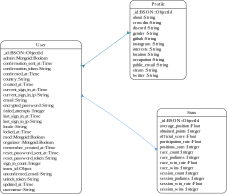
\includegraphics{datamodel1.png}
  \end{center}
  \caption[Modelo de relaciones entre usuario, perfil y estadísticas]{Modelo de relaciones entre usuario, perfil y estadísticas}
  \label{fig:datamodels1}
\end{figure}

\begin{figure}[H]
  \begin{center}
    \includegraphics{datamodel2.png}
  \end{center}
  \caption[Modelo de relación entre temporada, autos y pistas]{Modelo de relación entre temporada, autos y pistas}
  \label{fig:datamodels2}
\end{figure}

\begin{figure}[H]
  \begin{center}
    \includegraphics{datamodel3.png}
  \end{center}
  \caption[Modelo de relaciones entre temporada, ranking y sesiones con sus componentes]{Modelo de relaciones entre temporada, ranking y sesiones con sus componentes}
  \label{fig:datamodels3}
\end{figure}

\begin{figure}[H]
  \begin{center}
    \includegraphics{datamodel4.png}
  \end{center}
  \caption[Modelo de relación entre sesión, carrera y entrada de corredor]{Modelo de relación entre sesión, carrera y entrada de corredor}
  \label{fig:datamodels4}
\end{figure}

\newpage

\section{Esquema de la Base de Datos}
Todas las bases de datos dentro de MongoDB están prefijadas utilizando el término ''rv''. (Re-Volt) Por ejemplo, la base de datos que almacena las colecciones de autos se llama ''rv\_cars'', la de los usuarios ''rv\_users'', etc.

A continuación, se exponen fragmentos de código de Ruby con los modelos definidos para este proyecto. Los fragmentos de código están en formato de \textbf{mongoid} (librería de Ruby para MongoDB). Este formato se compone de la declaración de los campos de los modelos, especificando tipo y otras restricciones asociadas. Además, se mezcla el concepto de relaciones entre modelos de Ruby on Rails.

Para facilitar la comprensión de los esquemas de bases de datos a continuación, la siguiente tabla contiene una pequeña especificación de los atributos utilizados para definir los modelos.

\begin{center}
  \begin{tabular}{ | p{6cm} | p{11cm} |}
    \hline
    \multicolumn{1}{|c|}{\textbf{Atributo}} & \multicolumn{1}{|c|}{\textbf{Detalle}} \\
    \hline
    
    {\textbf{store\_in}} & Declara el nombre de la base de datos de mongo en donde los documentos de este modelo serán almacenados.\\ \hline
    {\textbf{field}} & Declara el nombre de un campo del modelo. \\ \hline
    {\textbf{embeds\_many}} & Declara que el modelo contendrá una colección de modelos anidados. \\ \hline
    {\textbf{accepts\_nested\_attributes\_for}} & Declara que el modelo aceptará atributos para los modelos anidados que éste contenga. \\ \hline
    {\textbf{validates\_presence\_of}} & Valida si el campo proveído no está vacío al momento de guardar el modelo en la base de datos. \\ \hline
    {\textbf{belongs\_to}} & Declara que el modelo tendrá una referencia por ID a otro modelo, quedando esta registrada como un atributo.
     \\ \hline
    {\textbf{has\_many}} & Declara que el modelo podrá ser referenciado por ID desde varios otros modelos. \\ \hline
    {\textbf{has\_one}} & Declara que el modelo contará con una referencia singular por ID a otro modelo. \\ \hline
    {\textbf{validates}} & Declara una o más validaciones para un campo del modelo, tales como su presencia garantizada, singularidad, tamaño mínimo o máximo, entre otras.\\ \hline
  \end{tabular}
\end{center}

\begin{listing}
  \begin{minted}[mathescape,
  	numbersep=5pt,
  	frame=single,
  	framesep=2mm]{ruby}
class Season
  include Mongoid::Document
  include Mongoid::Timestamps
  include Mongoid::MultiParameterAttributes
  
  store_in :database => 'rv_seasons'
  
  has_many :rankings
  has_many :cars
  has_many :tracks
  
  embeds_many :racer_result_entries
  
  accepts_nested_attributes_for :racer_result_entries
  
  field :name, :type => String
  field :start_date, :type => Date
  field :end_date, :type => Date
  field :current, :type => Boolean, :default => false
  
  validates_presence_of :name
  validates_presence_of :start_date
  validates_presence_of :current
  
  validates_uniqueness_of :name
end
  \end{minted}
  \caption[Esquema de Season]{Representación en código del modelo de Season de RVA.}
\end{listing}

\begin{listing}
\begin{minted}[mathescape,
	numbersep=5pt,
	gobble=2,
	frame=single,
	framesep=2mm]{ruby}
  class Ranking
    include Mongoid::Document
    include Mongoid::Timestamps
    
    store_in :database => 'rv_rankings'
    
    belongs_to :season
    has_many :sessions
    
    embeds_many :racer_result_entries
    
    accepts_nested_attributes_for :racer_result_entries
    
    field :number, :type => Integer
    
    validates_presence_of :number
	 end
\end{minted}
\caption[Esquema de Ranking]{Representación en código del modelo de Ranking de RVA.}
\end{listing}

\begin{listing}
  \begin{minted}[mathescape,
    numbersep=5pt,
    gobble=2,
    frame=single,
    framesep=2mm]{ruby}
    class Session
      include Mongoid::Document
      include SessionLogUploader::Attachment(:session_log)
      include Mongoid::Timestamps
      
      store_in :database => 'rv_sessions'
      
      belongs_to :ranking
      embeds_many :races
      embeds_many :racer_result_entries
      
      accepts_nested_attributes_for :racer_result_entries
      
      field :number, :type => Integer
      field :host, :type => String
      field :version, :type => String
      field :physics, :type => String
      field :protocol, :type => String
      field :pickups, :type => Boolean
      field :date, :type => Date
      field :teams, :type => Boolean
      field :category, :type => Integer
      field :session_log_data, :type => String
      
      validates_presence_of :number
      validates_presence_of :host
      validates_presence_of :version
      validates_presence_of :physics
      validates_presence_of :protocol
      validates_presence_of :date
      validates_presence_of :session_log
      validates_presence_of :teams
      validates_presence_of :category
    end
  \end{minted}
  \caption[Esquema de Session]{Representación en código del modelo de Session de RVA.}
\end{listing}

\begin{listing}
  \begin{minted}[mathescape,
    numbersep=5pt,
    gobble=2,
    frame=single,
    framesep=2mm]{ruby}
    class User
      include Mongoid::Document
      include Mongoid::Timestamps
      
      store_in :database => 'rv_users'
      
      USERNAME_REGEX = /\A([A-Z0-9_]{1,16}|[0-9a-f]{24})\z/
      
      validates :email, :presence => true, :uniqueness => true
      validates :username, :presence => true, 
        :uniqueness => true, 
        :length => { :minimum => 2, :maximum => 16 }
      validates_format_of :username, :with => USERNAME_REGEX
      
      belongs_to :team, :optional => true
      has_one :team
      
      embeds_one :profile
      embeds_one :stats
      accepts_nested_attributes_for(
        :profile,
        :update_only => true,
        :allow_destroy => false
      )
      accepts_nested_attributes_for(:stats,
        :update_only => true,
        :allow_destroy => false
      )
      
      before_create :create_profile
      before_create :create_stats
      
      field :admin, :type => Boolean, :default => false
      field :mod, :type => Boolean, :default => false
      field :organizer, :type => Boolean, :default => false
      field :locale, :type => String, :default => 'en_us'
      field :country, :type => String
    end
  \end{minted}
  \caption[Esquema de Session]{Representación en código del modelo de Session de RVA.}
\end{listing}

\begin{listing}
  \begin{minted}[mathescape,
    numbersep=5pt,
    gobble=2,
    frame=single,
    framesep=2mm]{ruby}
    class Race
      include Mongoid::Document
      include Mongoid::Attributes::Dynamic
      
      embedded_in :session
      
      embeds_many :racer_entries
      
      field :track_name, :type => String
      field :laps, :type => Integer
      field :racers_count, :type => Integer
      
      validates_presence_of :track_name
      validates_presence_of :laps
      validates_presence_of :racers_count
    end
  \end{minted}
  \caption[Esquema de Profile]{Representación en código del modelo Profile.}
\end{listing}

\begin{listing}
  \begin{minted}[mathescape,
    numbersep=5pt,
    gobble=2,
    frame=single,
    framesep=2mm]{ruby}
    class RacerEntry
      include Mongoid::Document
      include Mongoid::Attributes::Dynamic
      
      embedded_in :race
      
      field :car_name, :type => String
      field :position, :type => Integer
      field :username, :type => String
      field :time, :type => String
      field :best_lap, :type => String
      field :finished, :type => Mongoid::Boolean
      field :cheating, :type => Mongoid::Boolean
      
      validates_presence_of :car_name
      validates_presence_of :position
      validates_presence_of :username
      validates_presence_of :time
      validates_presence_of :best_lap
      validates_presence_of :finished
      validates_presence_of :cheating
    end
  \end{minted}
  \caption[Esquema de Profile]{Representación en código del modelo Profile.}
\end{listing}

\begin{listing}
  \begin{minted}[mathescape,
    numbersep=5pt,
    gobble=2,
    frame=single,
    framesep=2mm]{ruby}
    class Profile
      include Mongoid::Document
      
      embedded_in :user
      
      field :about, :type => String
      field :gender, :type => String
      field :public_email, :type => String
      field :location, :type => String
      field :discord, :type => String
      field :github, :type => String
      field :instagram, :type => String
      field :crowdin, :type => String
      field :steam, :type => String
      field :twitter, :type => String
      field :occupation, :type => String
      field :interests, :type => String
    end
  \end{minted}
  \caption[Esquema de Profile]{Representación en código del modelo Profile.}
\end{listing}

\begin{listing}
  \begin{minted}[mathescape,
    numbersep=5pt,
    gobble=2,
    frame=single,
    framesep=2mm]{ruby}
    class Stats
      include Mongoid::Document
      
      embedded_in :user
      
      field :race_wins, :type => Integer
      field :race_win_rate, :type => Float
      field :race_podiums, :type => Integer
      field :race_count, :type => Integer
      field :positions_sum, :type => Integer
      field :session_wins, :type => Integer
      field :session_win_rate, :type => Float
      field :session_podiums, :type => Integer
      field :session_count, :type => Integer
      field :average_position, :type => Float
      field :participation_rate, :type => Float
      field :official_score, :type => Float
      field :obtained_points, :type => Integer
    end
  \end{minted}
  \caption[Esquema de Stats]{Representación en código del modelo Stats.}
\end{listing}

\begin{listing}
  \begin{minted}[mathescape,
    numbersep=5pt,
    gobble=2,
    frame=single,
    framesep=2mm]{ruby}
    class Car
      include Mongoid::Document
      include Mongoid::Timestamps
      
      store_in :database => 'rv_cars'
      
      belongs_to :season
      
      field :name, :type => String
      field :speed, :type => Float
      field :accel, :type => Float
      field :weight, :type => Float
      field :multiplier, :type => Float
      field :folder_name, :type => String
      field :category, :type => Integer
      field :stock, :type => Boolean, :default => false
      
      validates_presence_of :name
      validates_presence_of :speed
      validates_presence_of :accel
      validates_presence_of :weight
      validates_presence_of :multiplier
      validates_presence_of :folder_name
      validates_presence_of :category
      validates_presence_of :stock
    end
  \end{minted}
  \caption[Esquema de Car]{Representación en código del modelo Car.}
\end{listing}

\begin{listing}
  \begin{minted}[mathescape,
    numbersep=5pt,
    gobble=2,
    frame=single,
    framesep=2mm]{ruby}
    class Track
      include Mongoid::Document
      include Mongoid::Timestamps
      
      store_in :database => 'rv_tracks'
      
      belongs_to :season
      
      field :name, :type => String
      field :short_name, :type => String
      field :difficulty, :type => Integer
      field :length, :type => Integer
      field :folder_name, :type => String
      field :stock, :type => Boolean, :default => false
      
      validates_presence_of :name
      validates_presence_of :short_name
      validates_presence_of :difficulty
      validates_presence_of :length
      validates_presence_of :folder_name
      validates_presence_of :stock
    end
  \end{minted}
  \caption[Esquema de Track]{Representación en código del modelo Track.}
\end{listing}

\begin{listing}
  \begin{minted}[mathescape,
    numbersep=5pt,
    gobble=2,
    frame=single,
    framesep=2mm]{ruby}
    class RacerResultEntry
      include Mongoid::Document
      
      embedded_in :season
      embedded_in :ranking
      embedded_in :session
      
      field :username, :type => String
      field :country, :type => String
      field :session_count, :type => Integer
      field :race_count, :type => Integer
      field :positions_sum, :type => Integer
      field :average_position, :type => Float
      field :obtained_points, :type => Integer
      field :official_score, :type => Float
      field :participation_multiplier, :type => Float
      field :team, :type => String
      
      validates_presence_of :username
      validates_presence_of :country
    end
  \end{minted}
  \caption[Esquema de Track]{Representación en código del modelo Track.}
\end{listing}

\clearpage

\section{Diseño de Interfaz}
El diseño de las interfaces de Re-Volt America ha sido debidamente cuidado al ser implementado en aplicación desarrollada.

En primer lugar, contamos con una página de inicio con el título de la comunidad de Re-Volt America, junto con varias imágenes del juego para que este pueda ser inmediatamente reconocido por quien visite el portal.

En la parte superior, se encuentra la barra de navegación principal, la cual incluye, de izquierda a derecha:
\begin{itemize}
  \item El logo de RVA.
  \item Botones para acceder a las secciones más importantes de la web.
  \item Un botón para poder registrarse, iniciar sesión o visualizar información del perfil en caso de existir una sesión iniciada.
\end{itemize}

\begin{figure}[H]
  \begin{center}
    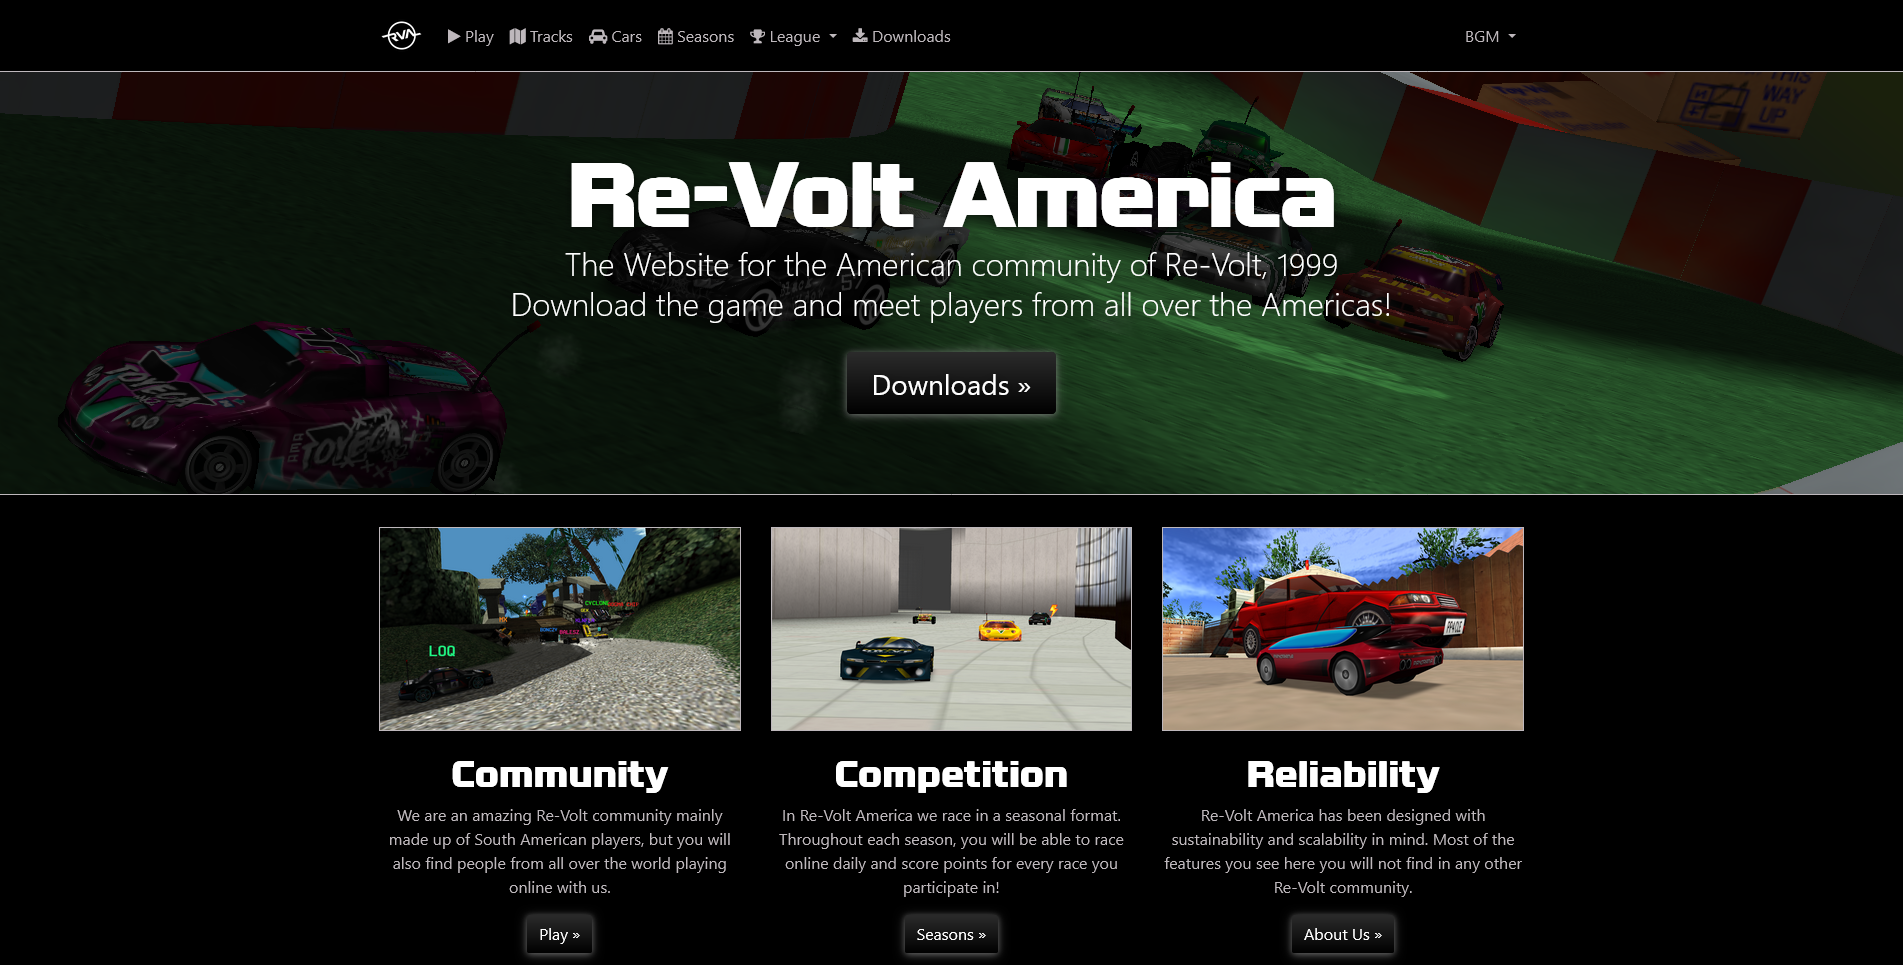
\includegraphics[width=15cm, height=8cm]{img/landing.png} 
  \end{center}
  \caption[Landing page de RVA]{Landing page de RVA}
  \label{fig:landing}
\end{figure}

Dentro de las secciones de autos, pistas y sesiones se cuenta con una barra de sub-navegación, la cual integra todos los elementos de una temporada, dando acceso al usuario de manera más práctica a toda la información que este podría necesitar.

\begin{figure}[H]
  \begin{center}
    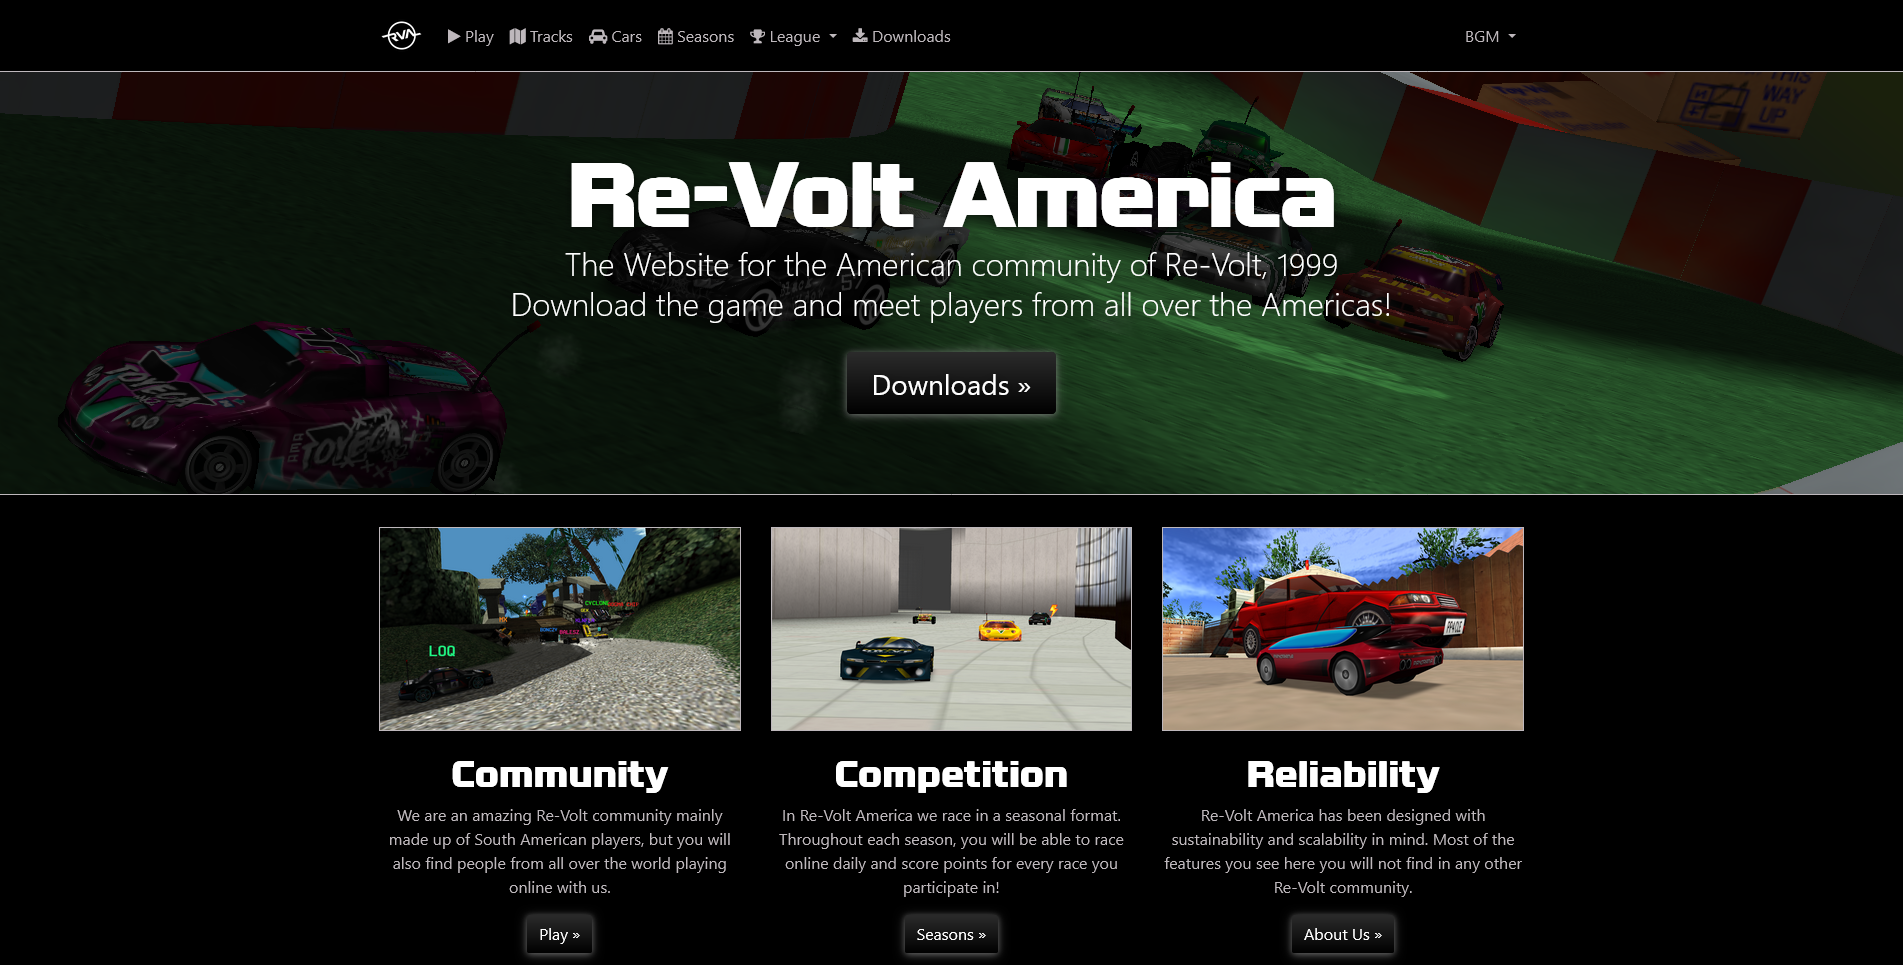
\includegraphics[width=15cm, height=8cm]{img/landing.png} 
  \end{center}
  \caption[Página de autos de RVA]{Página de autos de RVA}
  \label{fig:cars}
\end{figure}

\begin{figure}[H]
  \begin{center}
    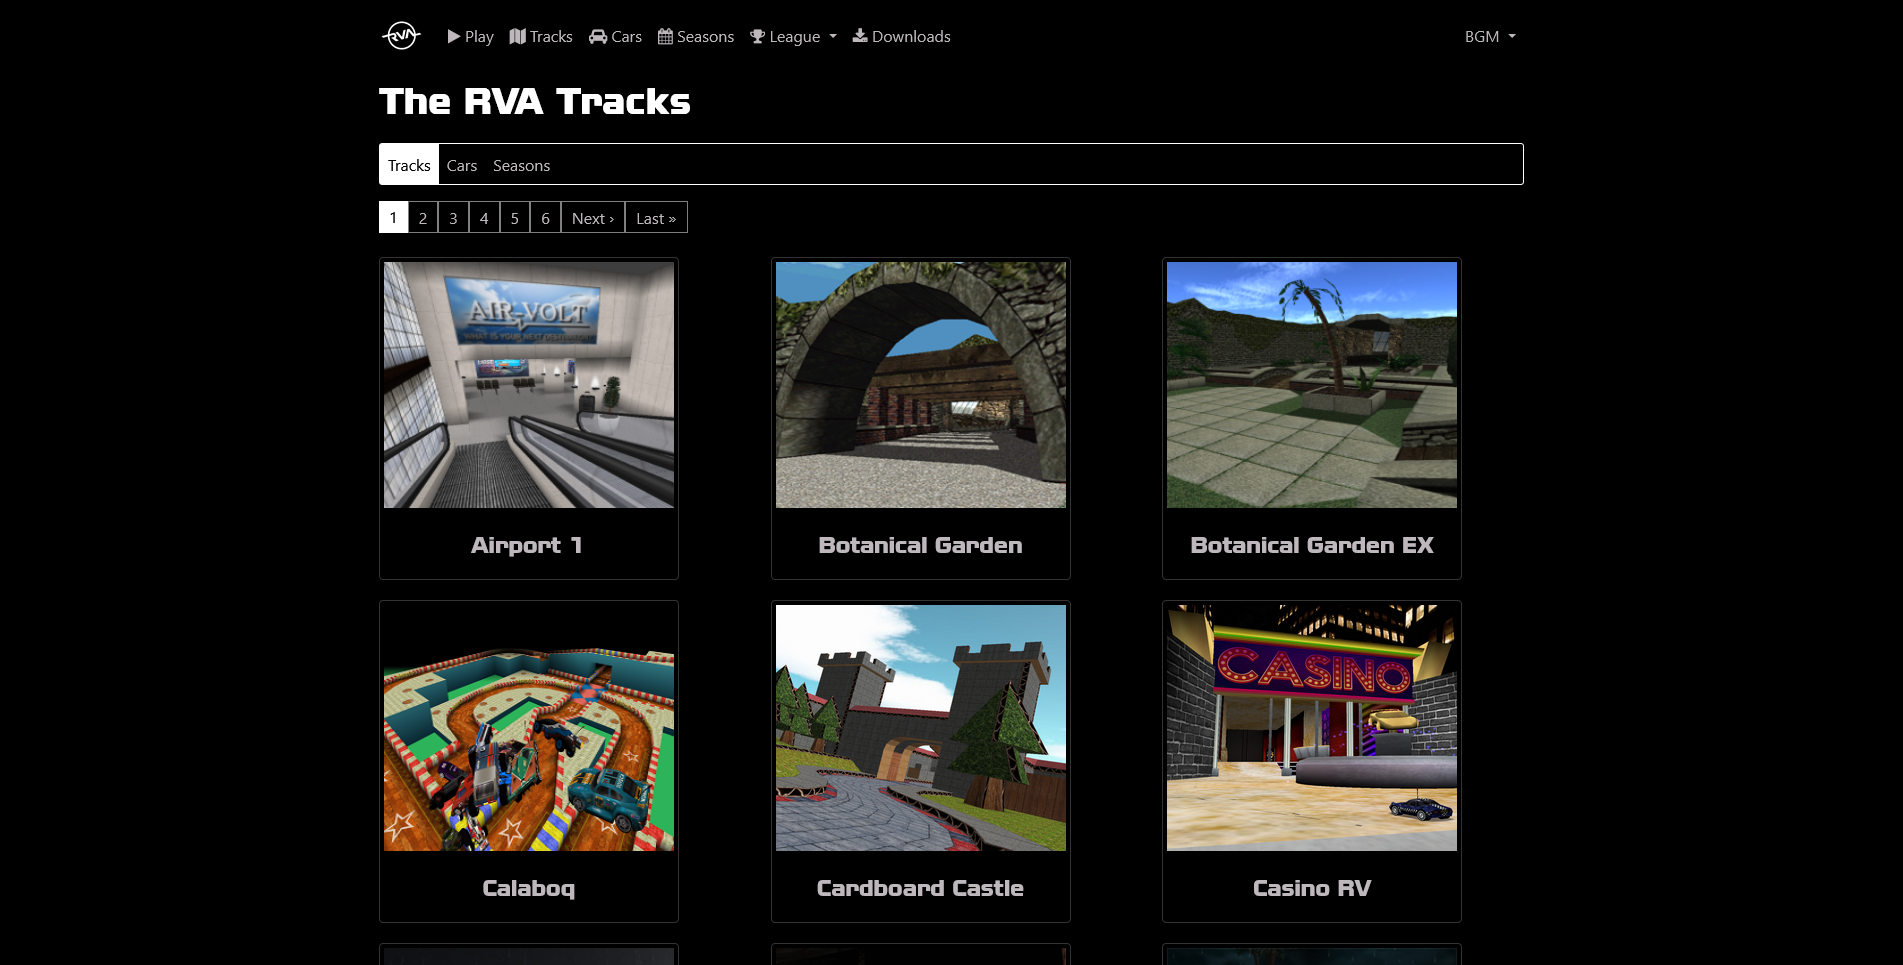
\includegraphics[width=15cm, height=8cm]{img/tracks.png} 
  \end{center}
  \caption[Página de pistas de RVA]{Página de pistas de RVA}
  \label{fig:tracks}
\end{figure}

El diseño de la interfaz de las sesiones respeta fielmente el formato original de RVA.

\begin{figure}[H]
  \begin{center}
    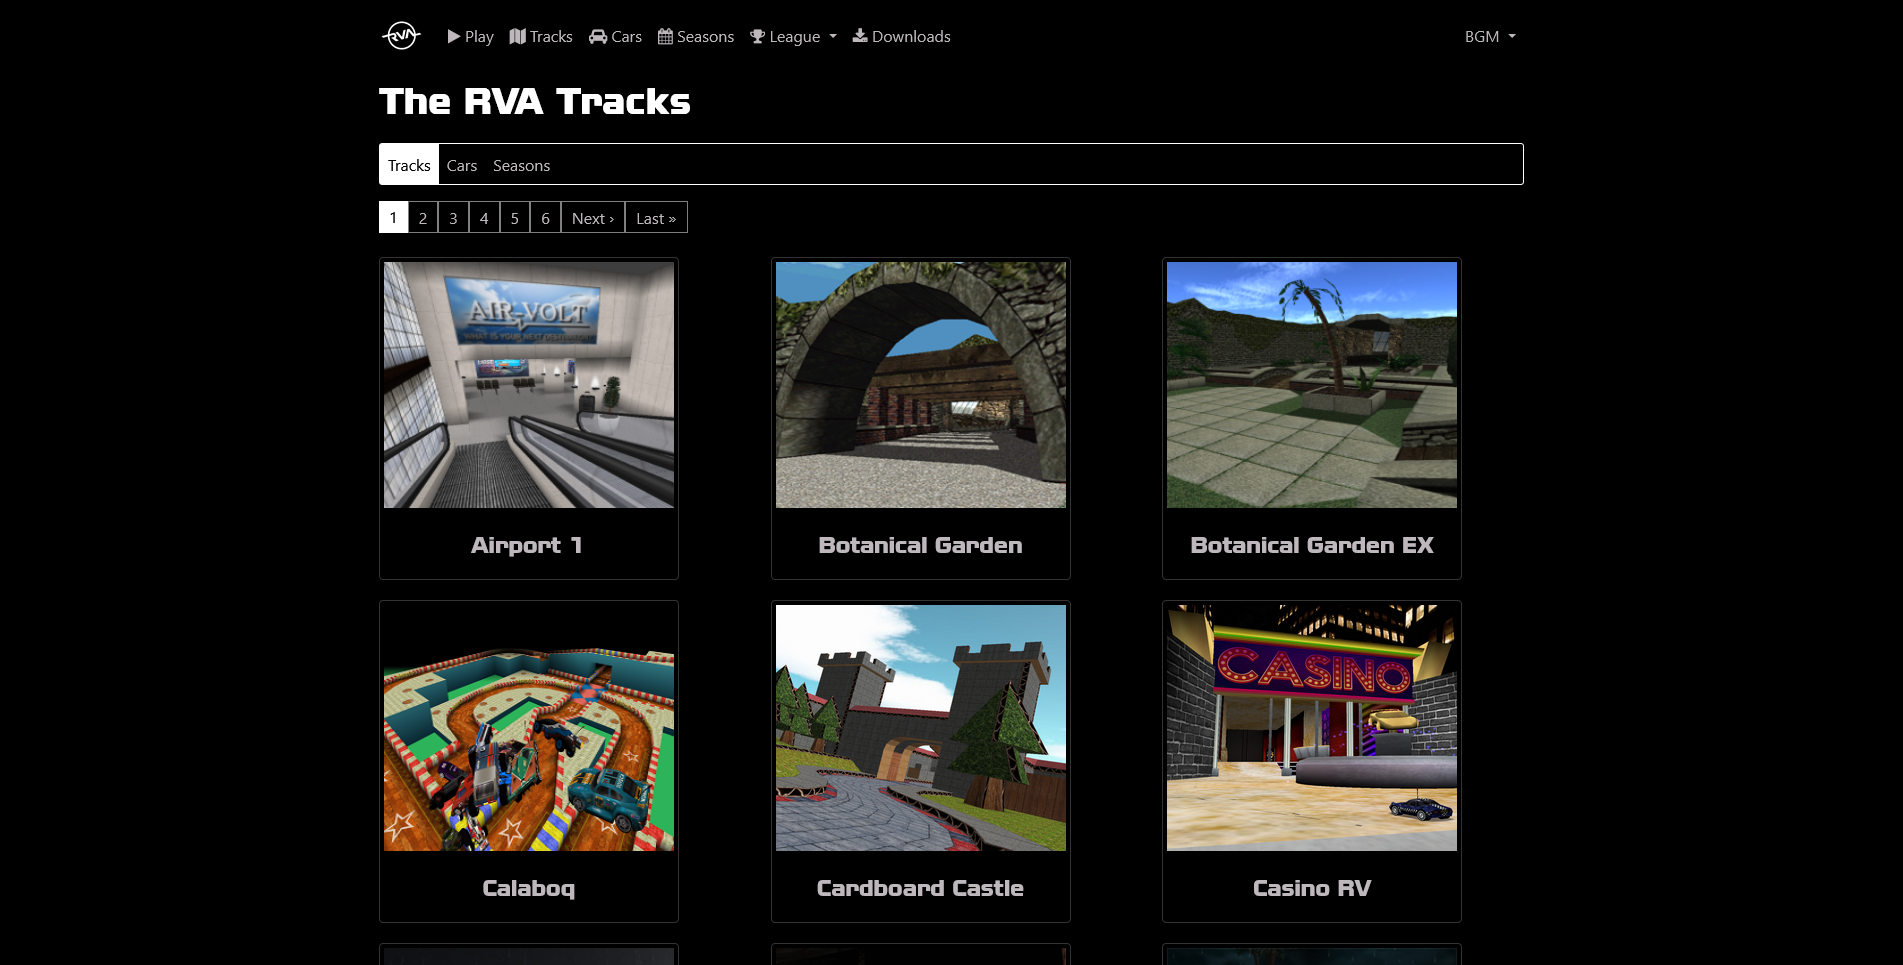
\includegraphics[width=15cm, height=8cm]{img/tracks.png} 
  \end{center}
  \caption[Página de sesión de RVA]{Página de sesión de RVA}
  \label{fig:session}
\end{figure}

La el diseño de la página de perfil de los usuarios cuenta con su nombre en grande, un resumen de sus estadísticas, posición en el ranking y un pequeño historial de las últimas sesiones en las que han participado.

\begin{figure}[H]
  \begin{center}
    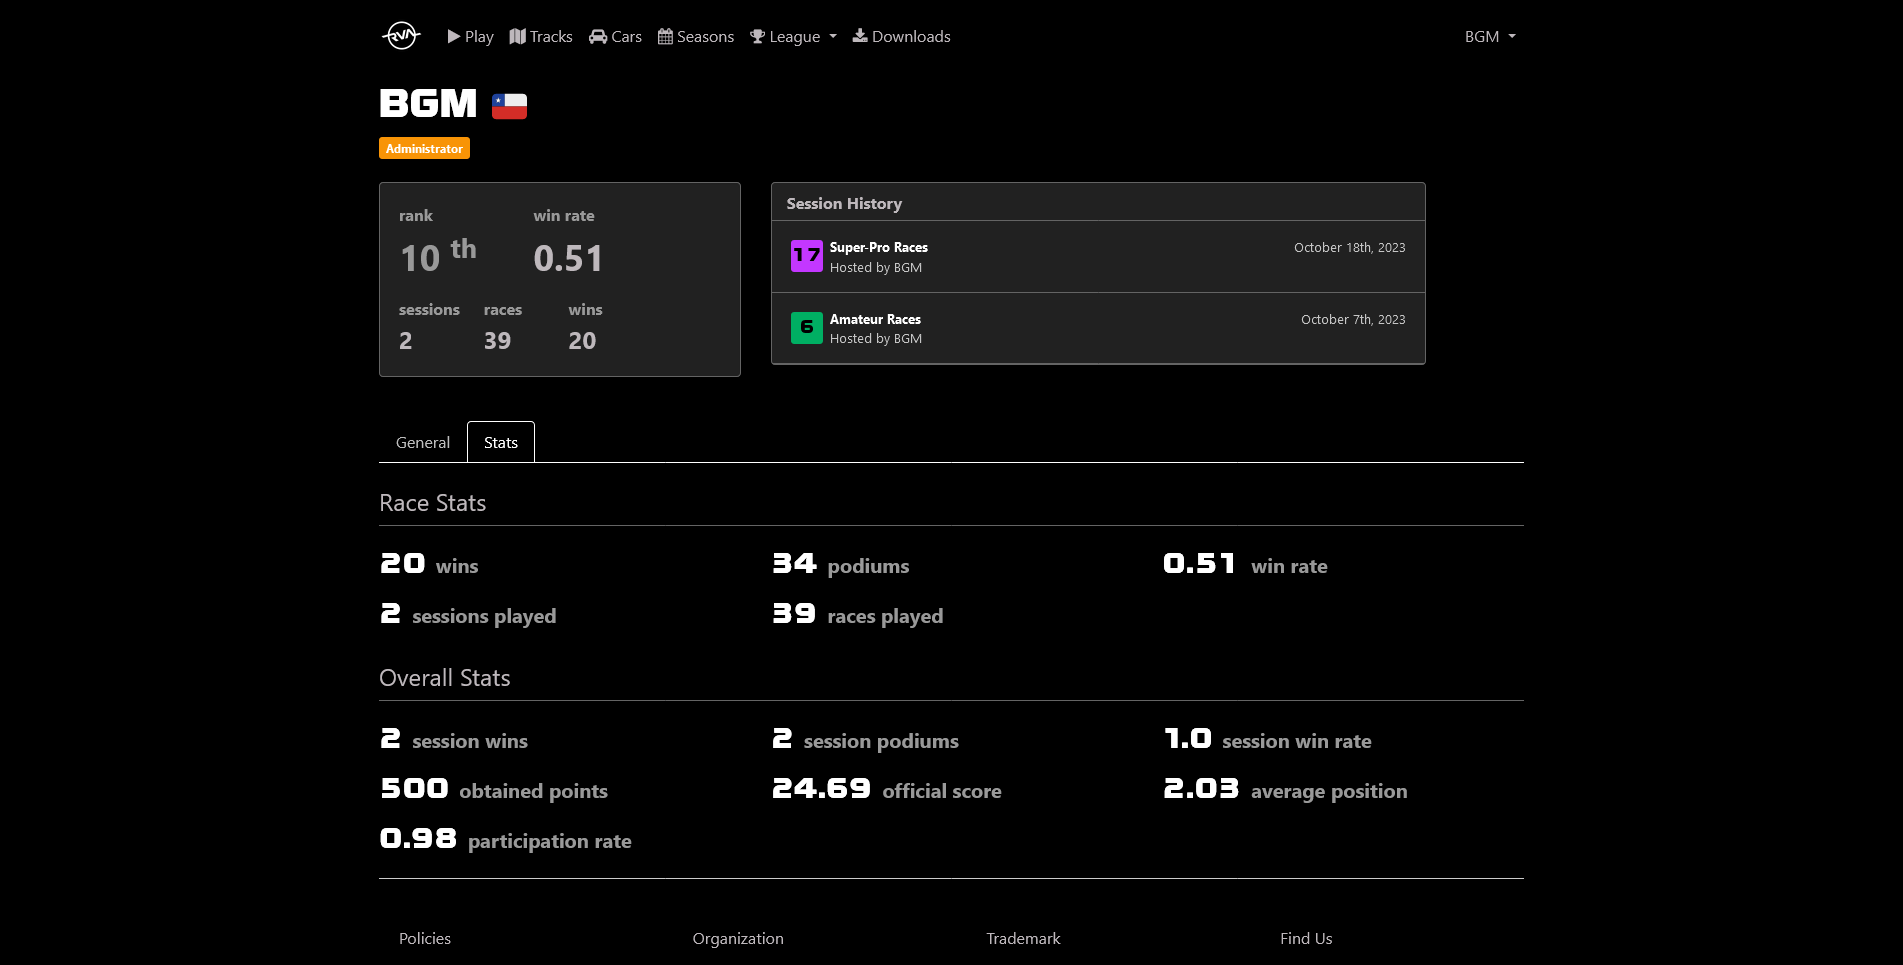
\includegraphics[width=15cm, height=8cm]{img/profile1.png} 
  \end{center}
  \caption[Página de perfil de usuario de RVA]{Página de perfil de usuario de RVA}
  \label{fig:profile}
\end{figure}

Por último, la página de estadísticas sigue un formato simple de tabla de resultados, con un selector que permite filtrar dichos resultados según diversos criterios.

\begin{figure}[H]
  \begin{center}
    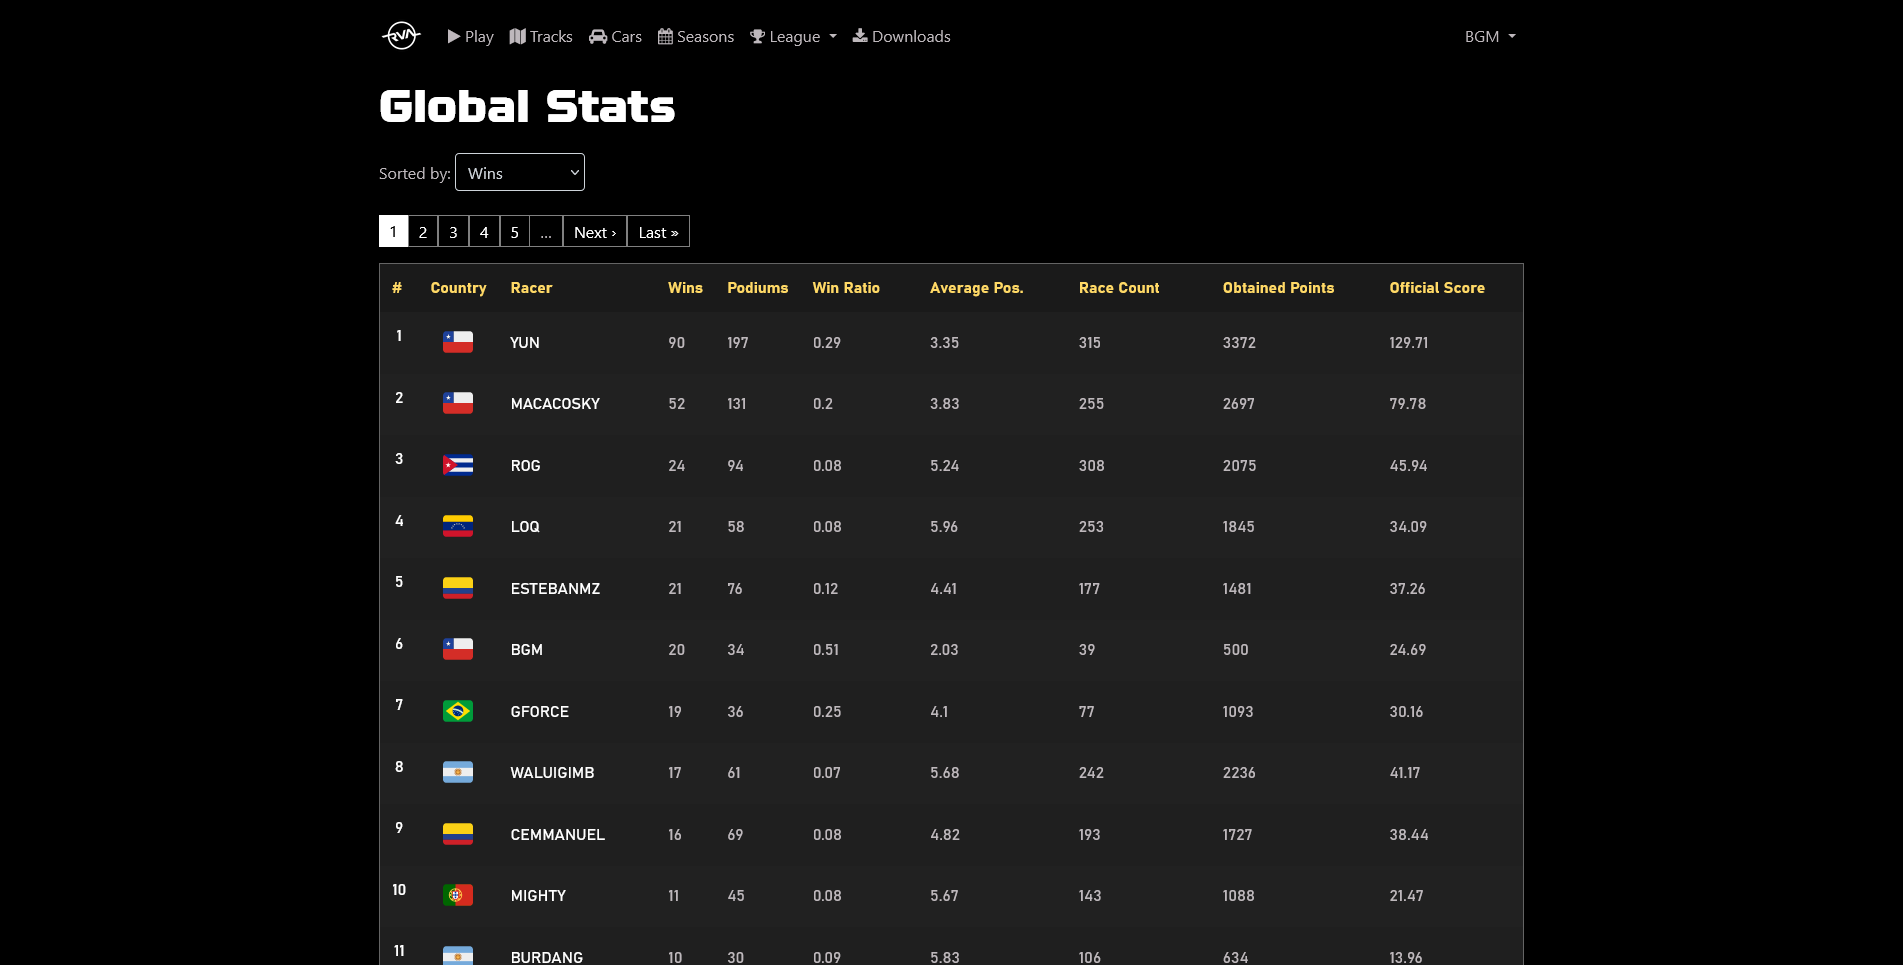
\includegraphics[width=15cm, height=8cm]{img/stats.png} 
  \end{center}
  \caption[Página de estadísticas globales de RVA]{Página de estadísticas globales de RVA}
  \label{fig:stats}
\end{figure}

\subsection{Paleta de Colores y Tipografía}
Como preámbulo principal en cuanto a la pelta de colores y tipografía de RVA, debemos recordar que esta comunidad nace de un grupo de jugadores de Re-Volt, no de una empresa o compañía con estándares definidos. Por lo tanto, para comprender los orígenes de estos elementos, debemos remontarnos a los inicios de Re-Volt America por el año 2017.

Durante los inicios de RVA, se diseña su logo principal, el cual puede apreciarse en la \autoref{fig:rva-logo}.

\begin{figure}[H]
  \begin{center}
    
\includegraphics[width=8cm, height=8cm]{img/rva.png} 
  \end{center}
  \caption[Logotipo de RVA]{Logotipo de RVA}
  \label{fig:rva-logo}
\end{figure}

Del logo de RVA, se derivan los colores blanco y negro (absolutos), los cuales son utilizados como paleta principal para la comunidad.

Así como los colores, la comunidad ha utilizado una fuente muy similar a la empleada en el logotipo a lo largo de los años. Esta fuente se titula ''Nissan Opti'', desarrollada originalmente por Castcraft Software. La caracterización de esta compañía tipográfica puede verse a continuación en la \autoref{fig:optifont}.

\begin{figure}[H]
  \begin{center}
    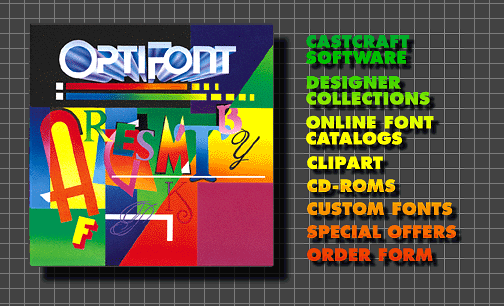
\includegraphics{img/optifont.png} 
  \end{center}
  \caption[Arte de Castcraft Software]{Arte de Castcraft Software}
  \label{fig:optifont}
\end{figure}

De la misma forma, nacen las paletas de colores para las tablas de resultados de sesiones y rankings acumulados. Estas últimas pueden apreciarse a continuación.


\begin{figure}[H]
  \begin{center}
    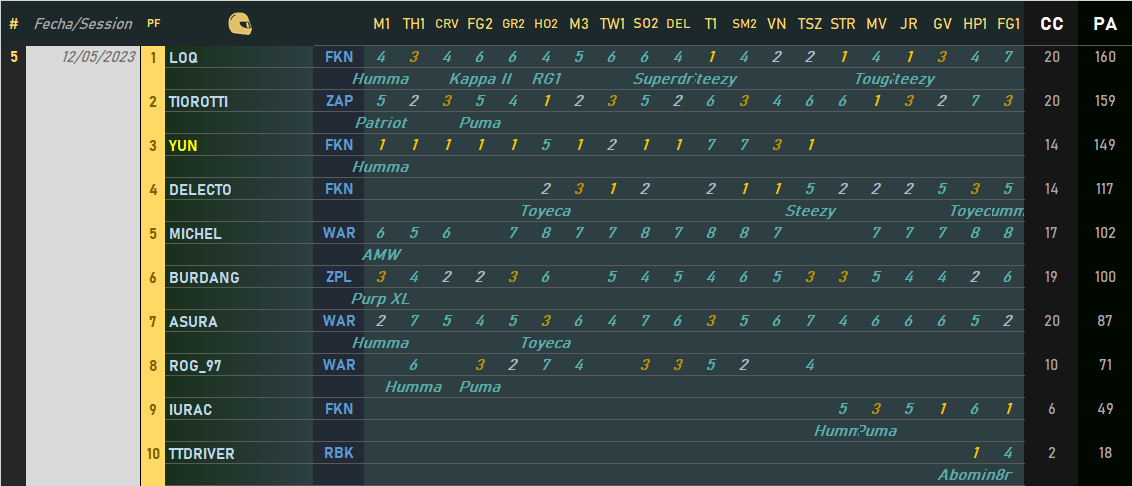
\includegraphics[width=16cm, height=11cm]{img/session_table.png} 
  \end{center}
  \caption[Tabla de resultados de sesión de RVA]{Tabla de resultados de sesión de RVA}
  \label{fig:session-table}
\end{figure}

\begin{figure}[H]
  \begin{center}
    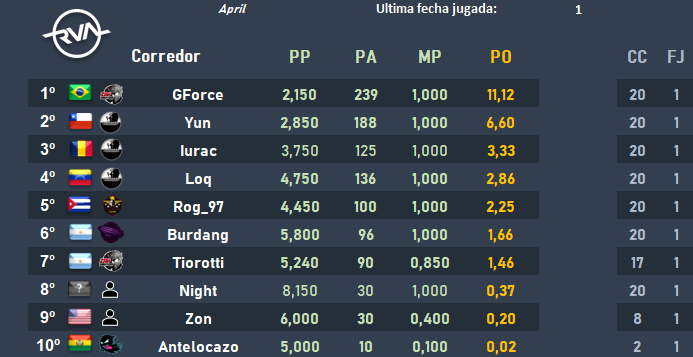
\includegraphics[width=16cm, height=11cm]{img/ranking_table.png} 
  \end{center}
  \caption[Tabla de ranking de RVA]{Tabla de ranking de RVA}
  \label{fig:ranking-table.png}
\end{figure}

La paleta de colores de las tablas de resultados, junto a su definición en RGB (Red, Green, Blue), puede encontrarse en la \autoref{fig:rva-session-colors} a continuación.

\begin{figure}[H]
  \begin{center}
    \includegraphics[width=15cm, height=10cm]{img/rva_session_colors.png} 
  \end{center}
  \caption[Paleta de colores de sesiones de RVA]{Paleta de colores de sesiones de RVA}
  \label{fig:rva-session-colors}
\end{figure}

\newpage

\section{Diseño de Arquitectura}
El proyecto, en su estado actual, hace uso de un servidor propio, el cual contiene los servicios web, bases de datos y caché. Todo en una sola máquina. Independientemente de donde se termine alojando, la aplicación web estará disponible en ''https://rva.lat/''.

Además de esto, la planificación contempla dos servicios externos, que actualmente son proveídos por GitHub pages, los cuales sirven como repositorios de almacenamiento de datos masivos. Dichos repositorios se encargan actualmente de servir información y assets como las imágenes de las pistas y autos que la web ofrece a los usuarios:

\begin{itemize}
	\item https://tracks.rva.lat/: Repositorio de pistas de RVA.
	\item https://cars.rva.lat/: Repositorio de autos de RVA.
\end{itemize}

A continuación, se muestra un diagrama que ilustra todo el proceso de interacción entre servicios y usuarios:

\begin{figure}[H]
  \begin{center}
    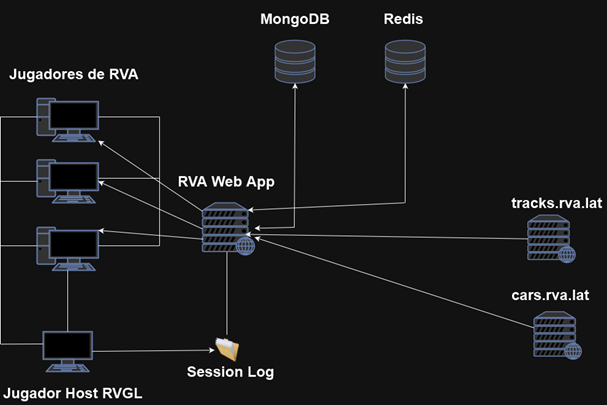
\includegraphics[width=16cm, height=11cm]{img/architecture.png} 
  \end{center}
  \caption[Diagrama de arquitectura de RVA]{Diagrama de arquitectura de RVA}
  \label{fig:architecture.png}
\end{figure}

Tal como se puede apreciar en la ilustración anterior, la arquitectura que da soporte a la aplicación web de RVA se concentra en un servidor, con dos almacenes de datos. Podemos ver que los usuarios juegan la sesión, el host de la sesión sube el Session Log a la web, y los usuarios pueden visitar la misma web para revisar los resultados

\newpage

\section{Estructura del Código}
El proyecto, al ser una aplicación hecha en el framework de Ruby on Rails, sigue el patrón de MVC (Model View Controller) o modelo, vista, controlador. El árbol de directorios del proyecto se ve de la siguiente manera.

\begin{figure}[H]
  \begin{center}
    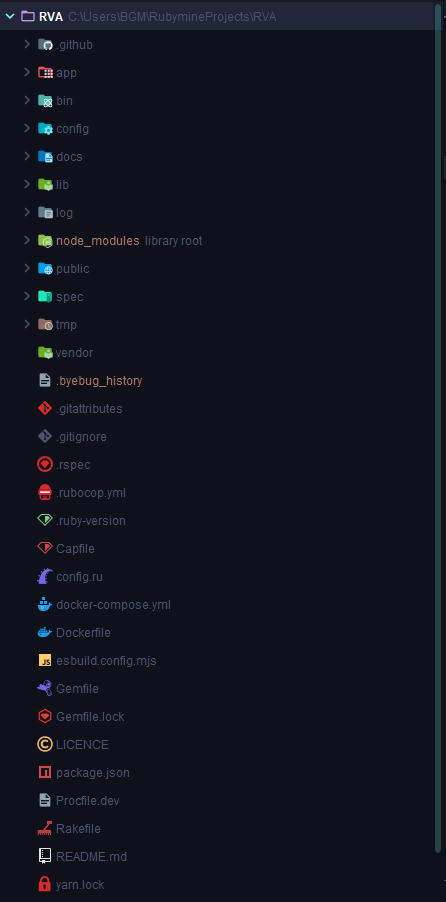
\includegraphics[height=16cm]{img/tree.png} 
  \end{center}
  \caption[Árbol de directorios del proyecto]{Árbol de directorios del proyecto}
  \label{fig:tree.png}
\end{figure}

Dentro los archivos relevantes para la estructura del código, tenemos aquellos archivos en los que se definen dependencias y módulos de despliegue.

\begin{center}
  \begin{tabular}{ | l | p{12.5cm} |}
    \hline
    \multicolumn{1}{|c|}{\textbf{Archivo}} & \multicolumn{1}{|c|}{\textbf{Detalle}} \\
    \hline
    
    {\textbf{Capfile}} & Contiene la carga de módulos para el despliegue de la aplicación. \\ \hline
    {\textbf{Gemfile}} & Contiene todas las dependencias del proyecto, con sus respectivas versiones. \\ \hline
  \end{tabular}
\end{center}

\subsection{Estándres de Codificación}
El código de este proyecto sigue las recomendaciones estándar para la programación con Ruby, y otros estándares de manera consistente:
\begin{itemize}
  \item Toda la base de código y documentación debe estar escrita en inglés.
  \item Eng eneral, todo el proyecto sigue las convenciones de nombrado y otros lineamientos útiles del sitio de RubyStyle.
  \item Se utilizan linebreaks (EOL - End of Line) CRLF.
  \item Se utilizan dos espacios para la indentación del código, no tabulaciones.
  \item La codificación del proyecto es en UTF-8. 
\end{itemize}

\subsection{Caché con Redis}
Las llaves o entradas del caché de Redis son nombradas en minúscula, y los espacios que pudieran existir en ellas son reemplazados por guiones bajos. En caso de llaves compuestas, se utiliza el siguiente formato:

\begin{itemize}
  \item \text{object\_type:id}
  \item \text{object\_type:id\#field}
  \item \text{object\_type:id\#embedded\_object:id}
  \item \text{object\_type:id\#embedded\_object:id\#field}
\end{itemize}

\begin{longlisting}
  \begin{minted}[mathescape,
    linenos,
    numbersep=5pt,
    breaklines,
    frame=single,
    framesep=2mm]{ruby}  
def show
  require 'rva_calculate_results_service'
  
  @count = 0
  @rva_results = Rails.cache.fetch("Session:#{@session.id}") do
    RvaCalculateResultsService.new(@session).call
  end
  
  respond_with @session do |format|
    format.json { render :layout => false }
  end
end
\end{minted}
  \caption[Ejemplo de Caché en Código]{Implementación de caché con Redis en Rails (\textit{sessions\_controller.rb})}
\end{longlisting}


\subsection{Backend}

\begin{center}
  \begin{tabular}{ | l | p{12.5cm} |}
    \hline
    \multicolumn{1}{|c|}{\textbf{Directorio}} & \multicolumn{1}{|c|}{\textbf{Detalle}} \\
    \hline
    
    {\textbf{controllers}} & Contiene todos los controladores de Rails, los cuales manejan todas las peticiones web del usuario. \\ \hline
    
    {\textbf{helpers}} & Contiene todas las clases utilitarias, las cuales pueden ser utilizadas para asistir a las clases de modelos, vistas y controladores. \\ \hline
    
    {\textbf{javascript}} & Todo el código de JavaScript utilizado por la aplicación a nivel web se almacena en este directorio.\\ \hline
    
    {\textbf{models}} & Contiene todas las clases que modelan y envuelven los datos almacenados en la base de datos de la aplicación. \\ \hline
    
    {\textbf{services}} & Contiene todas las clases de servicio de la aplicación. Las clases de servicio son aquellos procesos complejos compuestos de mucho código, los cuales se abstraen en servicios para no polucionar los controladores que los requieren. \\ \hline
    
    {\textbf{uploaders}} & Contiene todas las clases relacionadas con la subida de archivos. \\ \hline
    
    {\textbf{config}} & Contiene toda la configuración de la aplicación, como las rutas, inicializadores de librerías, configuración de despliegue, declaración de los entornos de Rails (development, production), configuración de la base de datos y archivos de idioma para la localización del proyecto.\\ \hline
  \end{tabular}
\end{center}

\subsection{Frontend}

\begin{center}
  \begin{tabular}{ | l | p{12.5cm} |}
    \hline
    \multicolumn{1}{|c|}{\textbf{Directorio}} & \multicolumn{1}{|c|}{\textbf{Detalle}} \\
    \hline
    
    {\textbf{views}} & Contiene todas las vistas de la aplicación. Todo lo que el usuario ve en la aplicación web tiene su archivo de vista que lo representa. \\ \hline
    
    {\textbf{assets}} & Todas las imágenes, hojas de estilo y demás artefactos requeridos por la aplicación para su correcto funcionamiento y diseño. \\ \hline
    
    {\textbf{public}} & Todos los archivos estáticos servidos por la página pueden encontrarse aquí. Cosas como las páginas de error (404, 422, 500, etc.), estilos compilados, entre otros.\\ \hline
  \end{tabular}
\end{center}


% Conclusión
\chapter{Conclusión del Proyecto}
Para finalizar este informe, a continuación, se plantean una serie de conclusiones a las que se llegó luego de llevar a cabo el desarrollo e implementación del software:

\begin{itemize}
	\item En relación con poder haber elaborado una propuesta que consiguiera atender las necesidades y problemas de los usuarios de Re-Volt America en relación con el almacenamiento y visualización de resultados de partidas online, podemos decir que, en conclusión, se logró cumplir dicho objetivo gracias al software desarrollado.
	\item De acuerdo con el objetivo que hablaba de diseñar una solución de software de procesamiento de datos de sesiones multijugador oficiales de las sesiones de carreras en línea, además de estadísticas personales, podemos decir que es un objetivo que fue cumplido parcialmente, ya que aún no se han implementado las estadísticas por jugador.
	\item En relación con el objetivo de implementar una aplicación web que permitiera a los organizadores de sesiones de carreras en línea subir y publica los resultados de dichas carreras podemos decir que, en conclusión, dicho objetivo fue cumplido con éxito, ya que el software, incluso en su estado actual, ya puede realizar la importación de Session Logs, el cálculo y procesamiento de resultados en el formato de RVA, y finalmente mostrar dichos resultados por pantalla a quien los solicite desde la web.
	\item El proyecto ha permitido demostrar, incluso en su estado actual, las competencias que se esperan de un ingeniero de ejecución en computación e informática, ya que he aplicado la identificación de necesidades, análisis y el diseño de soluciones informáticas para Re-Volt America, logrando desarrollar una solución que le permite a la comunidad tener un mejor manejo de sus proceso internos, registros de datos más fiables y una experiencia de usuario muchísimo mejor que con la que contaban al trabajar con su sistema original. 
	\item Bajo mi percepción, el proyecto fue realmente enriquecedor desde el punto de vista del desarrollo de software puesto que, dentro del área que fue comprendido pude aplicar diversas tecnologías, técnicas de diseño de software, despliegue de aplicaciones y aplicación de estándares de calidad, todo en un mismo contexto que cierra de manera redonda el ciclo de desarrollo que se espera pueda ser alcanzado por un ingeniero de software.
\end{itemize}

\subsection{Proyecciones del Proyecto}
Dentro de las proyecciones del proyecto etc etc


% Anexos
\chapter{Anexos}

\section{Anexo Estimación de Casos de Uso}

\section{Anexos de Recopilación de Información}
Para la recopilación de información de este proyecto, se realizaron varias reuniones en modalidad remota con la administración de RVA. En las 3 reuniones realizadas, se le hicieron preguntas a la administración tanto para conocer su opinión acerca de la facilidad de uso del software que estaba en desarrollo, como para que tuvieran la oportunidad de sugerir cambios o mejoras de interfaz o usabilidad del sitio.

Además de las reuniones por llamada, también se creó un chat de texto en línea con los administradores, organizadores y moderadores que contaban con el tiempo para poder participar de el. En este chat, continuarían entregando sus opiniones a lo largo del desarrollo del software propuesto, mientras que también se les mostraban avances del proyecto.

\section{Anexo Aspectos de Gestión de Proyectos}

\subsection{Anexo Carta Gantt}

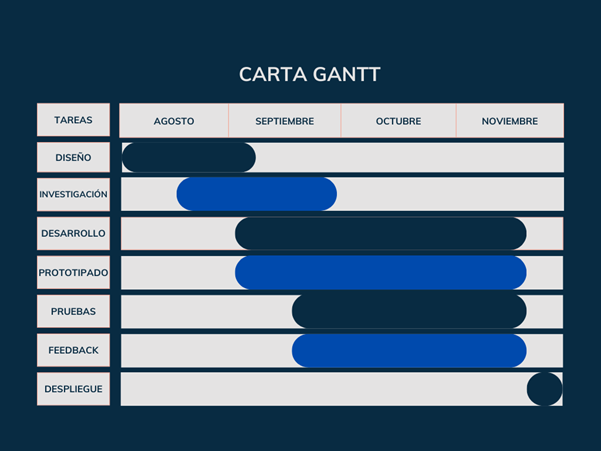
\includegraphics{gantt.png}

\subsection{Anexo Resumen de Esfuerzo}
\begin{center}
  \begin{tabular}{ | p{10cm} | p{5cm} |}
    \hline
    \multicolumn{1}{|c|}{\textbf{Actividad}} & \multicolumn{1}{|c|}{\textbf{Número de Horas}} \\
    \hline
    
    {Preparación del proyecto} & {20} \\ \hline
    {Desarrollo del módulo de autos} & {50} \\ \hline
    {Desarrollo del módulo de pistas} & {50} \\ \hline
    {Desarrollo del módulo de sesiones} & {80} \\ \hline
    {Desarrollo del módulo de temporadas} & {80} \\ \hline
    {Corrección de errores de código} & {40} \\ \hline
    {Despliegue de la aplicación} & {27} \\ \hline
    {Control de versiones} & {37} \\ \hline
    
    {\textbf{Total}} & {\textbf{384}} \\

    \hline
  \end{tabular}
\end{center}

\newpage

\section{Anexos Retrospectiva del Proyecto}

\subsection{Anexo Iteraciones en el Desarrollo}

\begin{center}
  \begin{tabular}{ | p{6cm} | p{3cm} | p {6cm} |}
    \hline
    \multicolumn{1}{|c|}{\textbf{Funcionalidad}} & \multicolumn{1}{|c|}{\textbf{Fecha}} &
    \multicolumn{1}{|c|}{\textbf{Retroalimentación}} \\
    \hline
    
    {Módulo de Autos (1)} & {12/11/2023} & {Añadir visualización para todos los autos y un sólo auto.}\\
    {Módulo de Autos (2)} & {12/11/2023} & {Agregar los autos tanto a la navegación como a la sub-navegación de la aplicación}\\
    {Módulo de Autos (3)} & {21/11/2023} & {Corregir problemas internos del modelo de autos}\\ \hline
   
    {Módulo de Pistas (1)} & {11/11/2023} & {Corregir problemas de validación en el modelo de Pista}\\
    {Módulo de Pistas (2)} & {12/11/2023} & {Agregaron las pistas tanto a la navegación como a la sub-navegación de la aplicación}\\
    {Módulo de Pistas (3)} & {28/11/2023} & {Mejorar la relación a modelos de Pista desde la visualización del modelo de Sesión.}\\ \hline
    
    {Módulo de Temporadas (1)} & {19/11/2023} & {Generar modelos de Ranking asociados a la temporada automáticamente después de crearla}\\
    {Módulo de Temporadas (2)} & {30/11/2023} & {Eliminar entradas de resultado de jugador asociadas a la temporada si estas tienen todos sus parámetros en cero}\\
    
    {Módulo de Sesiones (1)} & {19/11/2023} & {Determinar el número de cada sesión automáticamente una vez creada}\\
    {Módulo de Sesiones (2)} & {28/11/2023} & {Añadir botón de descarga para el Session Log asociado a cada sesión}\\
    {Módulo de Sesiones (3)} & {29/11/2023} & {Añadir acciones de administrador a la vista de sesión, tales como eliminar}\\
    
    \hline
  \end{tabular}
\end{center}


\end{document}




















